\chapter{Results}
 
\section{Mesh movement}
 
First, we show qualitatively the results for large deformation of a 2D unstructured linear mesh. In figure \ref{fig:wing-inviscid}, we show the undeformed mesh. In each of the results that follow, the flap of the wing has been rotated anti-clockwise by 60 degrees. We take note of the quality of triangular cells in these results. By `quality', we mean deviation of the angles of the triangle from 60$^\circ$, that is, the shape metric (sec. \ref{sec:lin-mesh-quality}), for this test case.
\begin{figure}
  	\centering
  	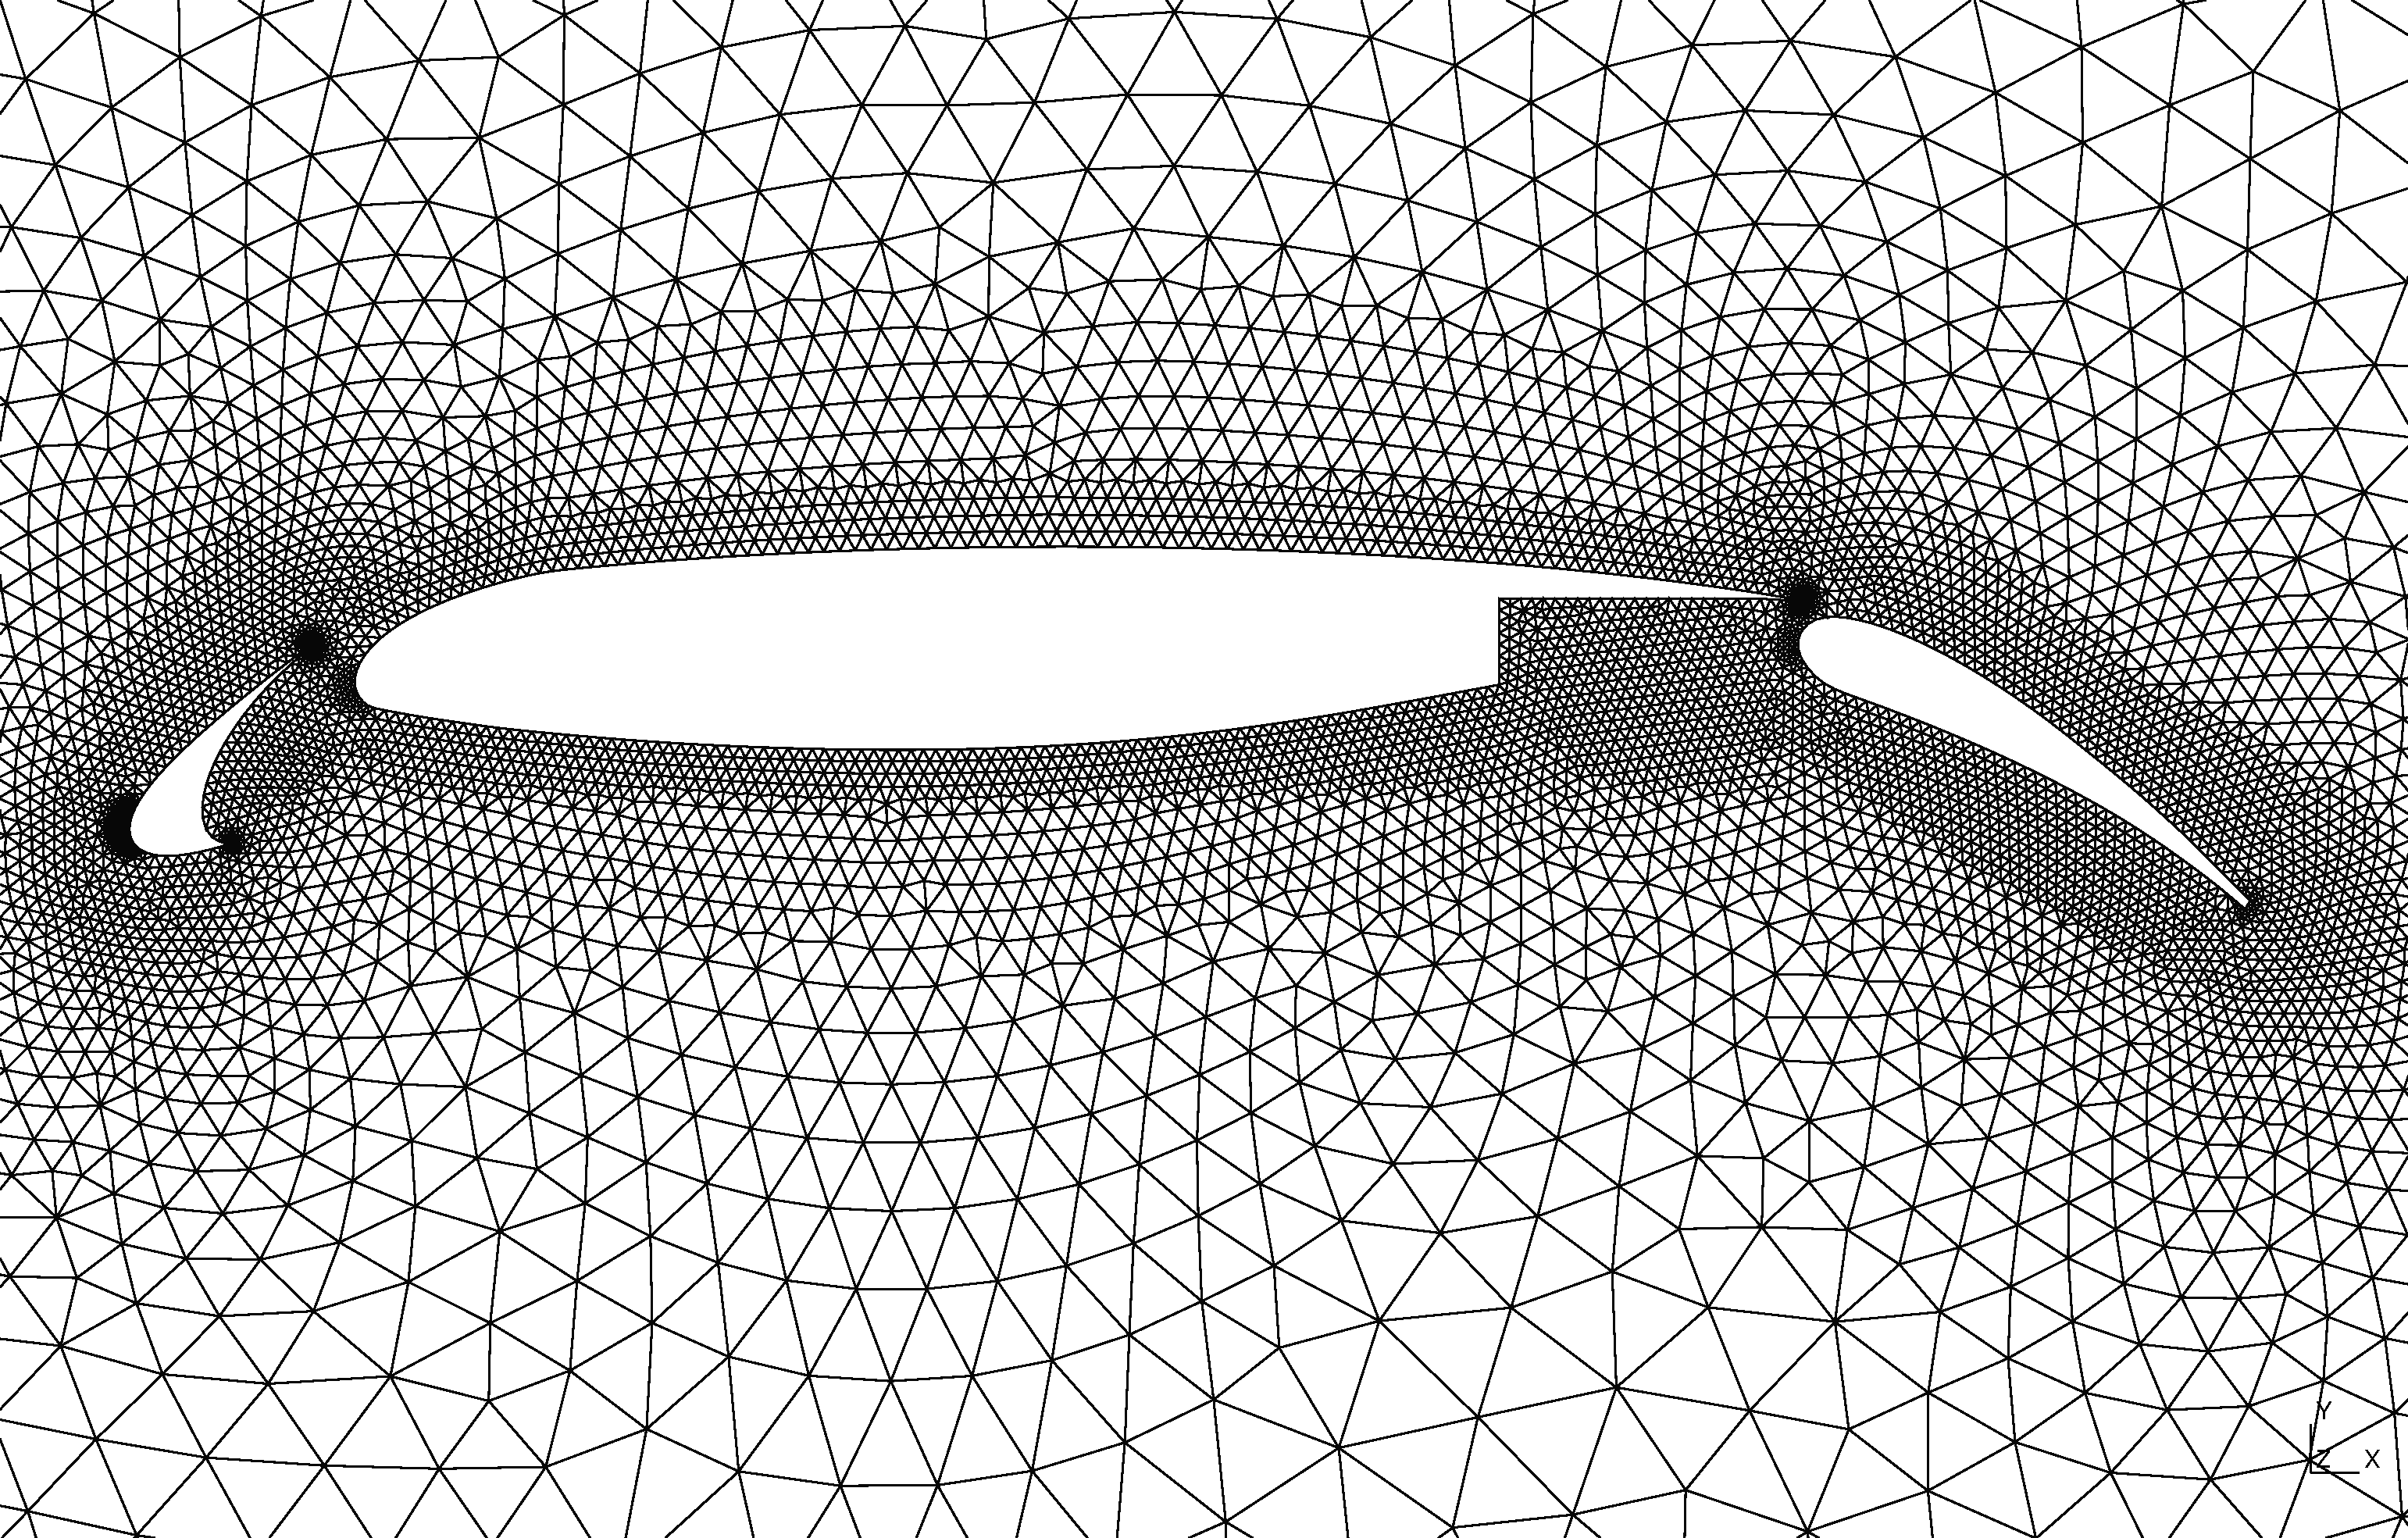
\includegraphics[scale=0.25]{3comp-inviscid}
  	\caption{Original mesh for inviscid flow around 3-component airfoil}
  	\label{fig:wing-inviscid}
\end{figure}

In figure \ref{fig:wing-inviscid-farhat}, we show the result of the torsion spring method of Farhat et. al. \cite{mm:torsionsprings}. We see that the result for such a large deformation is not acceptable; it is evident that there are invalid cells. It is interesting to note that cells near the trailing edge of the middle wing do not suffer much degradation, but cells somewhat farther away become invalid. Cells near the trailing edge of the flap also suffer large distortions.

\begin{figure}
	\centering
	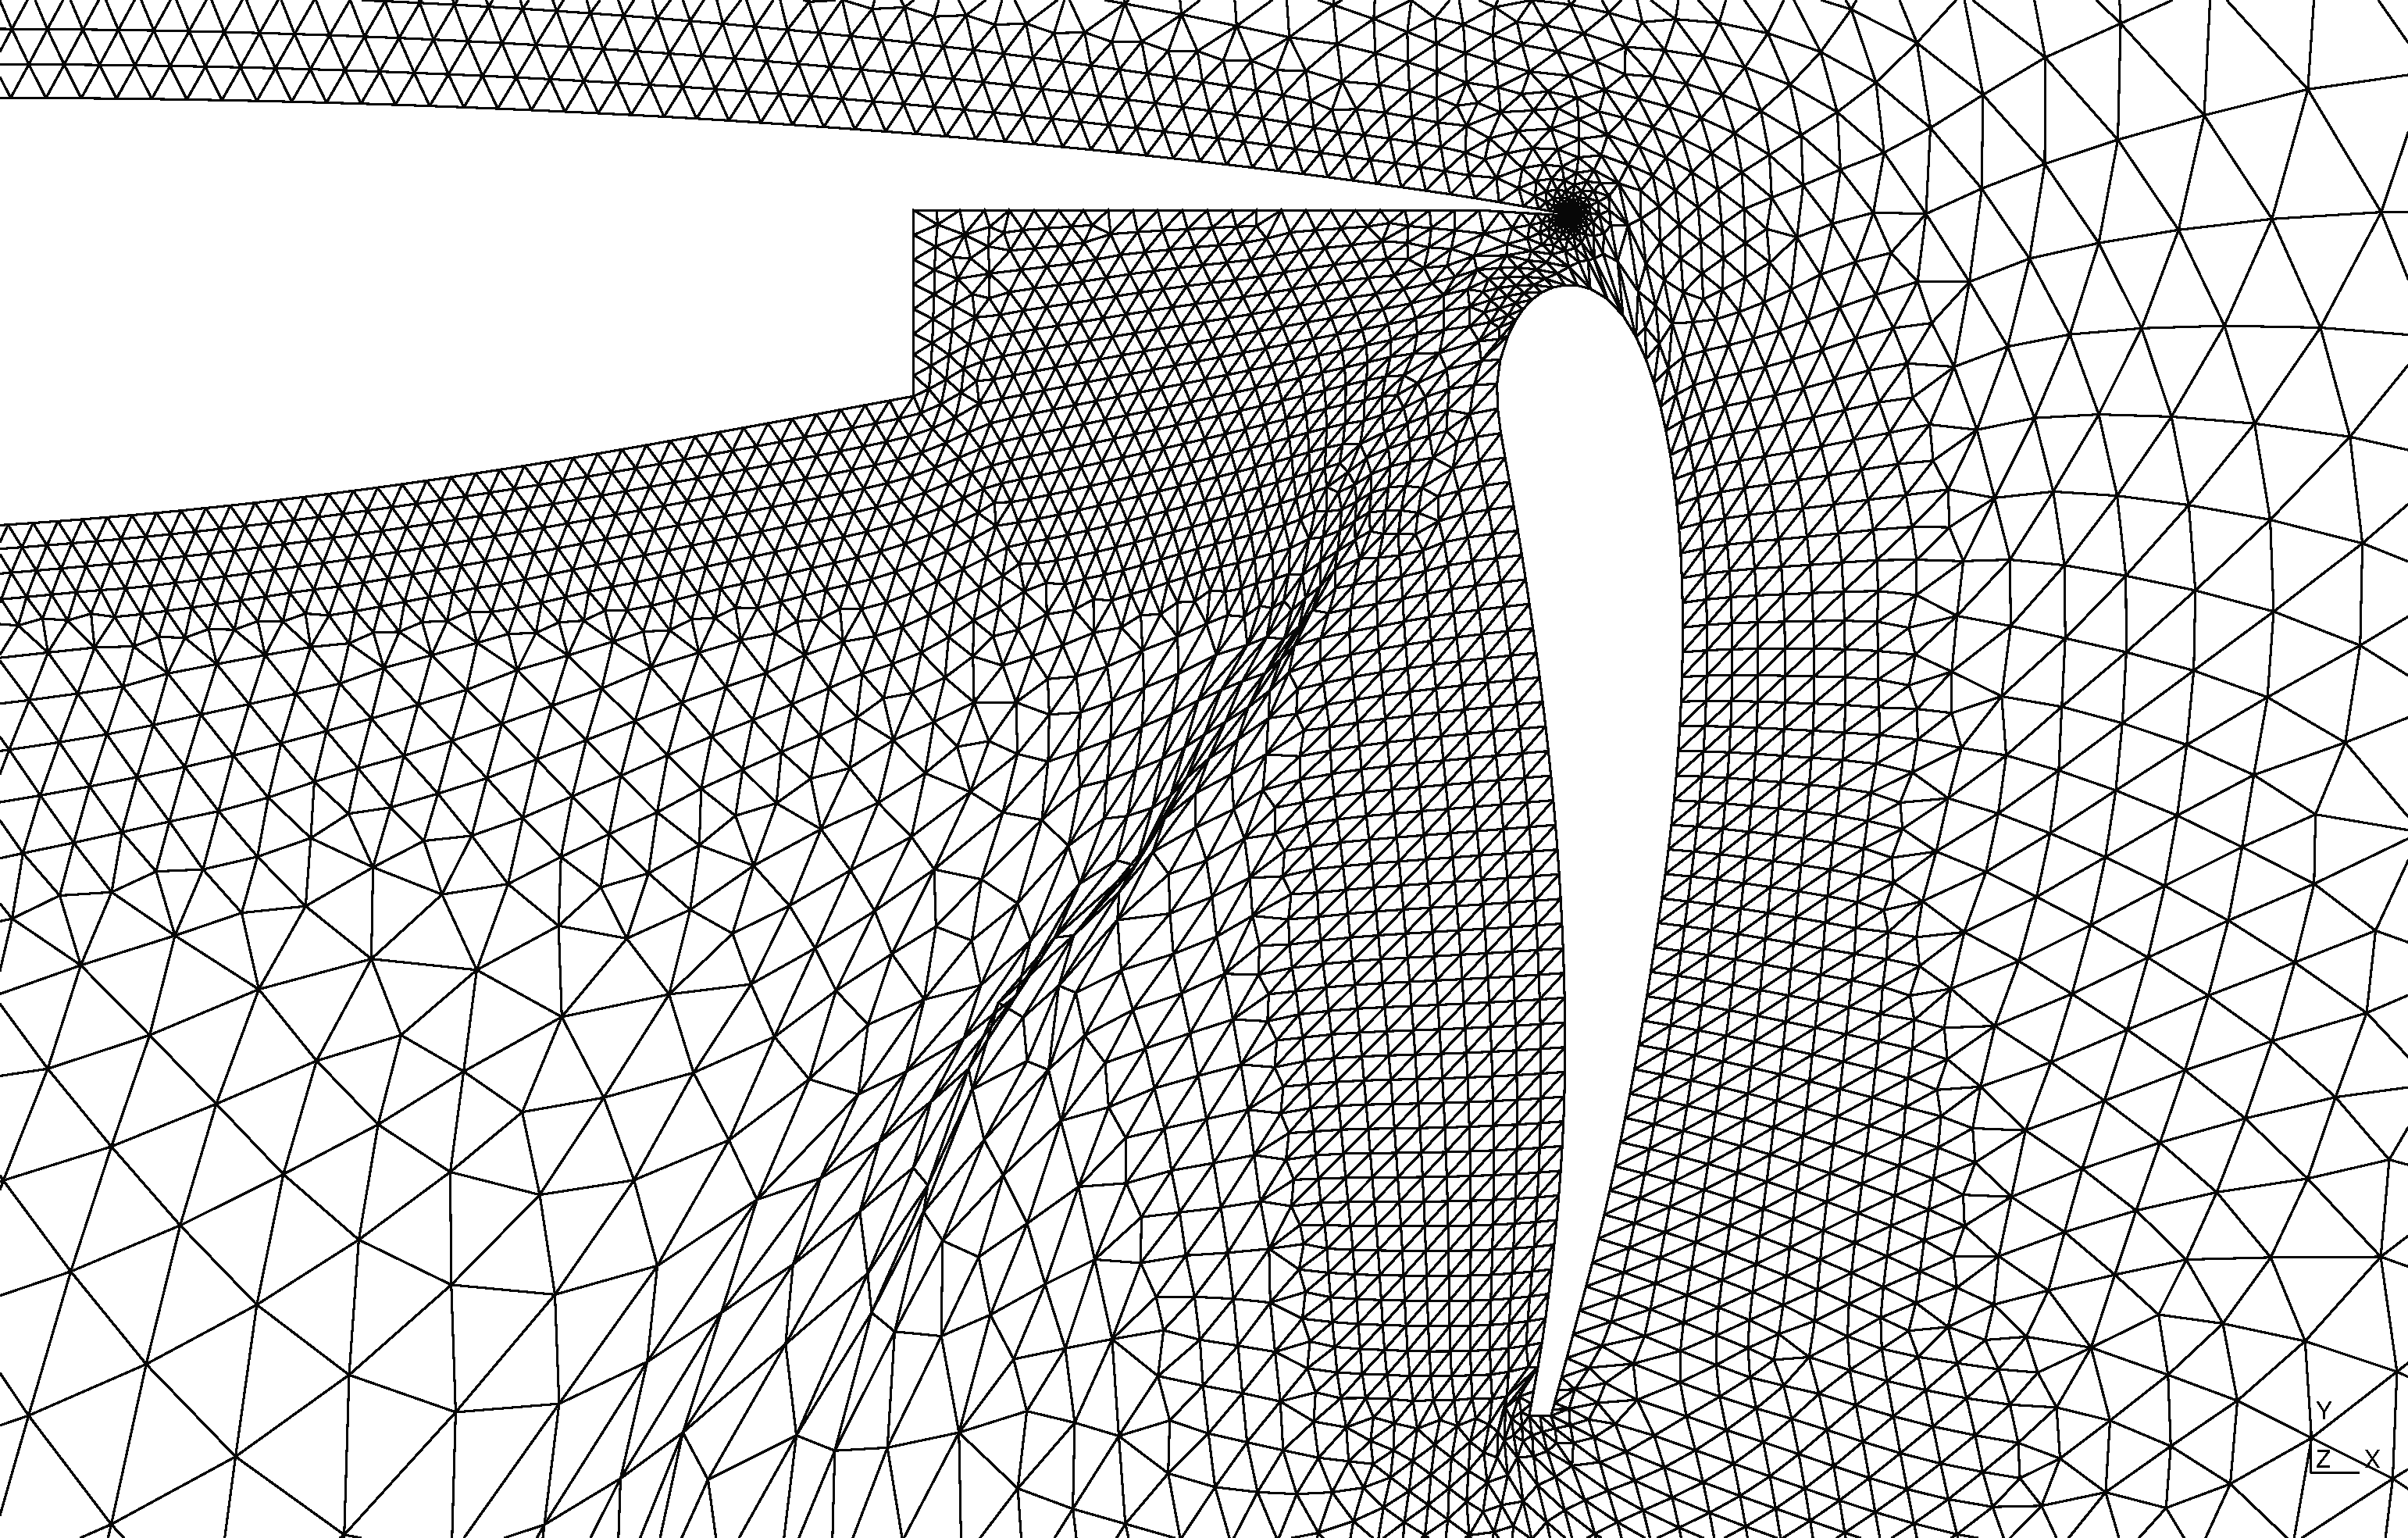
\includegraphics[scale=0.25]{wing60-farhat}
	\caption{Inviscid 3-component airfoil mesh with 60$^\circ$ rotation of flap by torsion spring method}
	\label{fig:wing-inviscid-farhat}
\end{figure}

Next, results of mesh movement by linear elasticity method are shown in figures \ref{fig:wing-inviscid-linelastp1}, \ref{fig:wing-inviscid-linelastp1-zoomed} and \ref{fig:wing-inviscid-linelastp1-zoomed2}. The mesh is valid; however, it suffers from nearly-degenerate cells near the trailing edge of the flap \ref{fig:wing-inviscid-linelastp1-zoomed2}. This could seriously impact the performance, accuracy and even stability of flow solvers using this mesh. In figure \ref{fig:wing-inviscid-linelastp1-zoomed}, we  see that the quality of cells is better than near the trailing edge, but not very good.

\begin{figure}
	\centering
	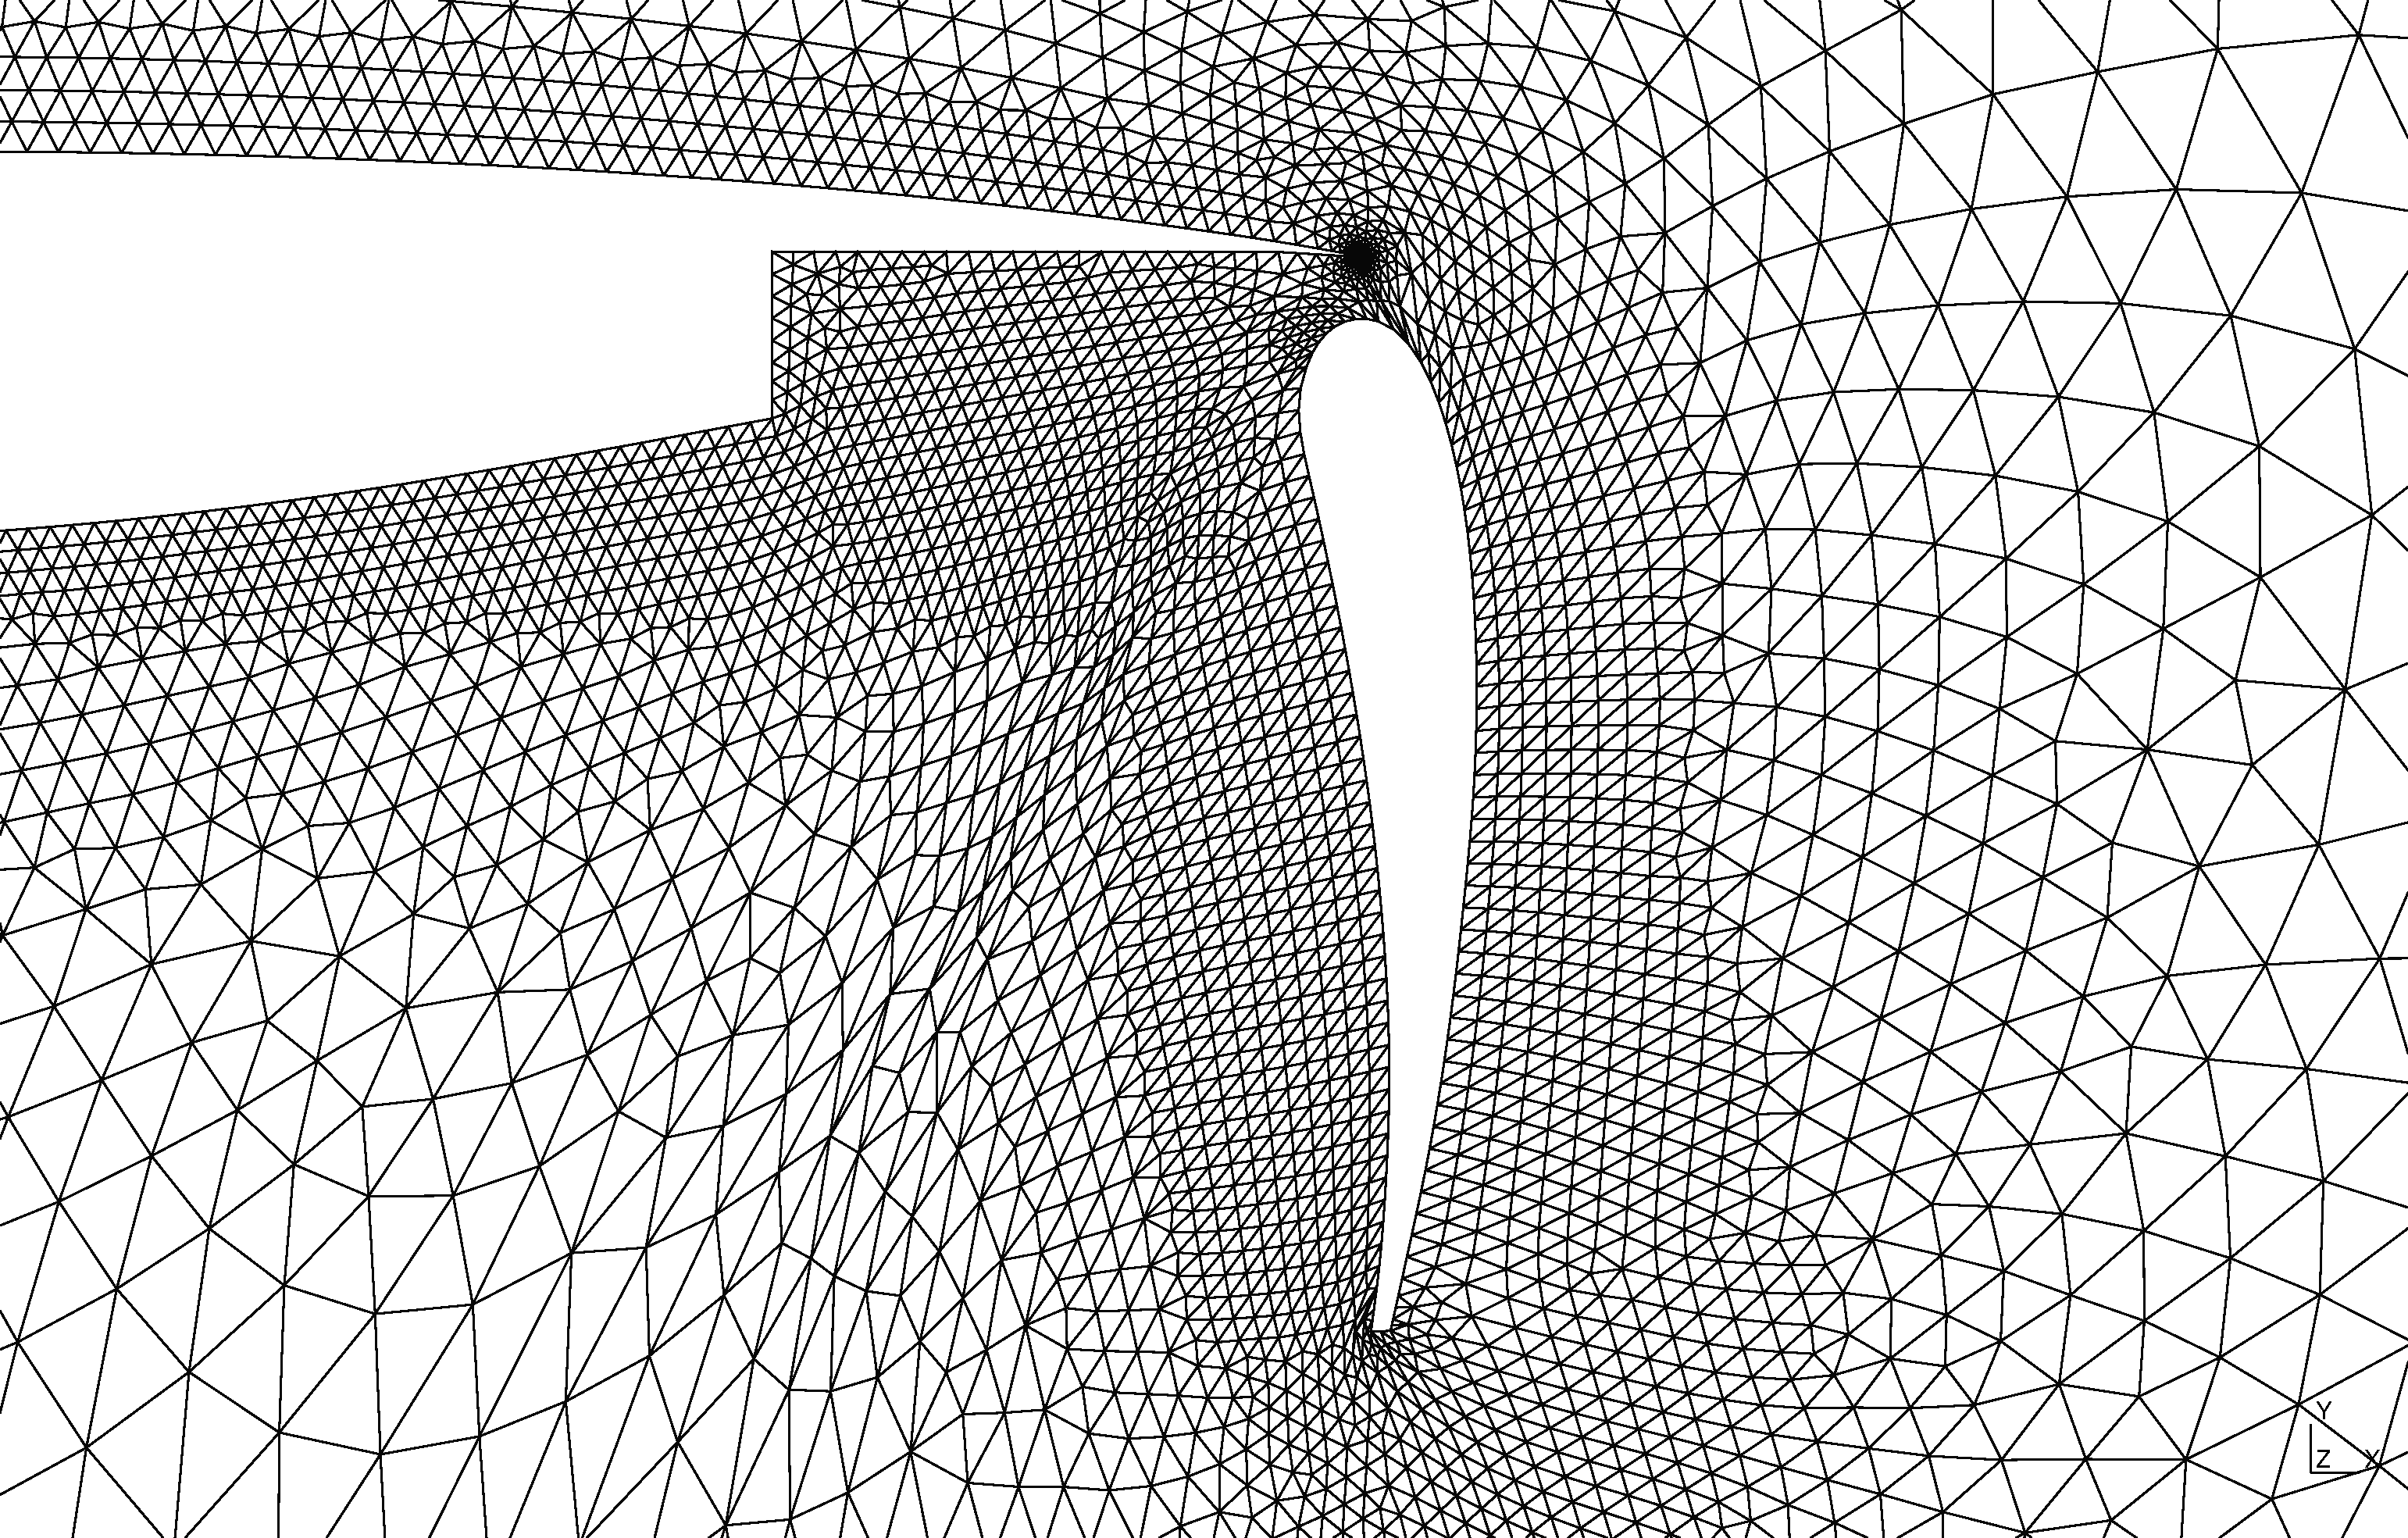
\includegraphics[scale=0.25]{wing60-linelastp1}
	\caption{Inviscid 3-component airfoil mesh with 60$^\circ$ rotation of flap by linear elasticity method}
	\label{fig:wing-inviscid-linelastp1}
\end{figure}
\begin{figure}
	\centering
	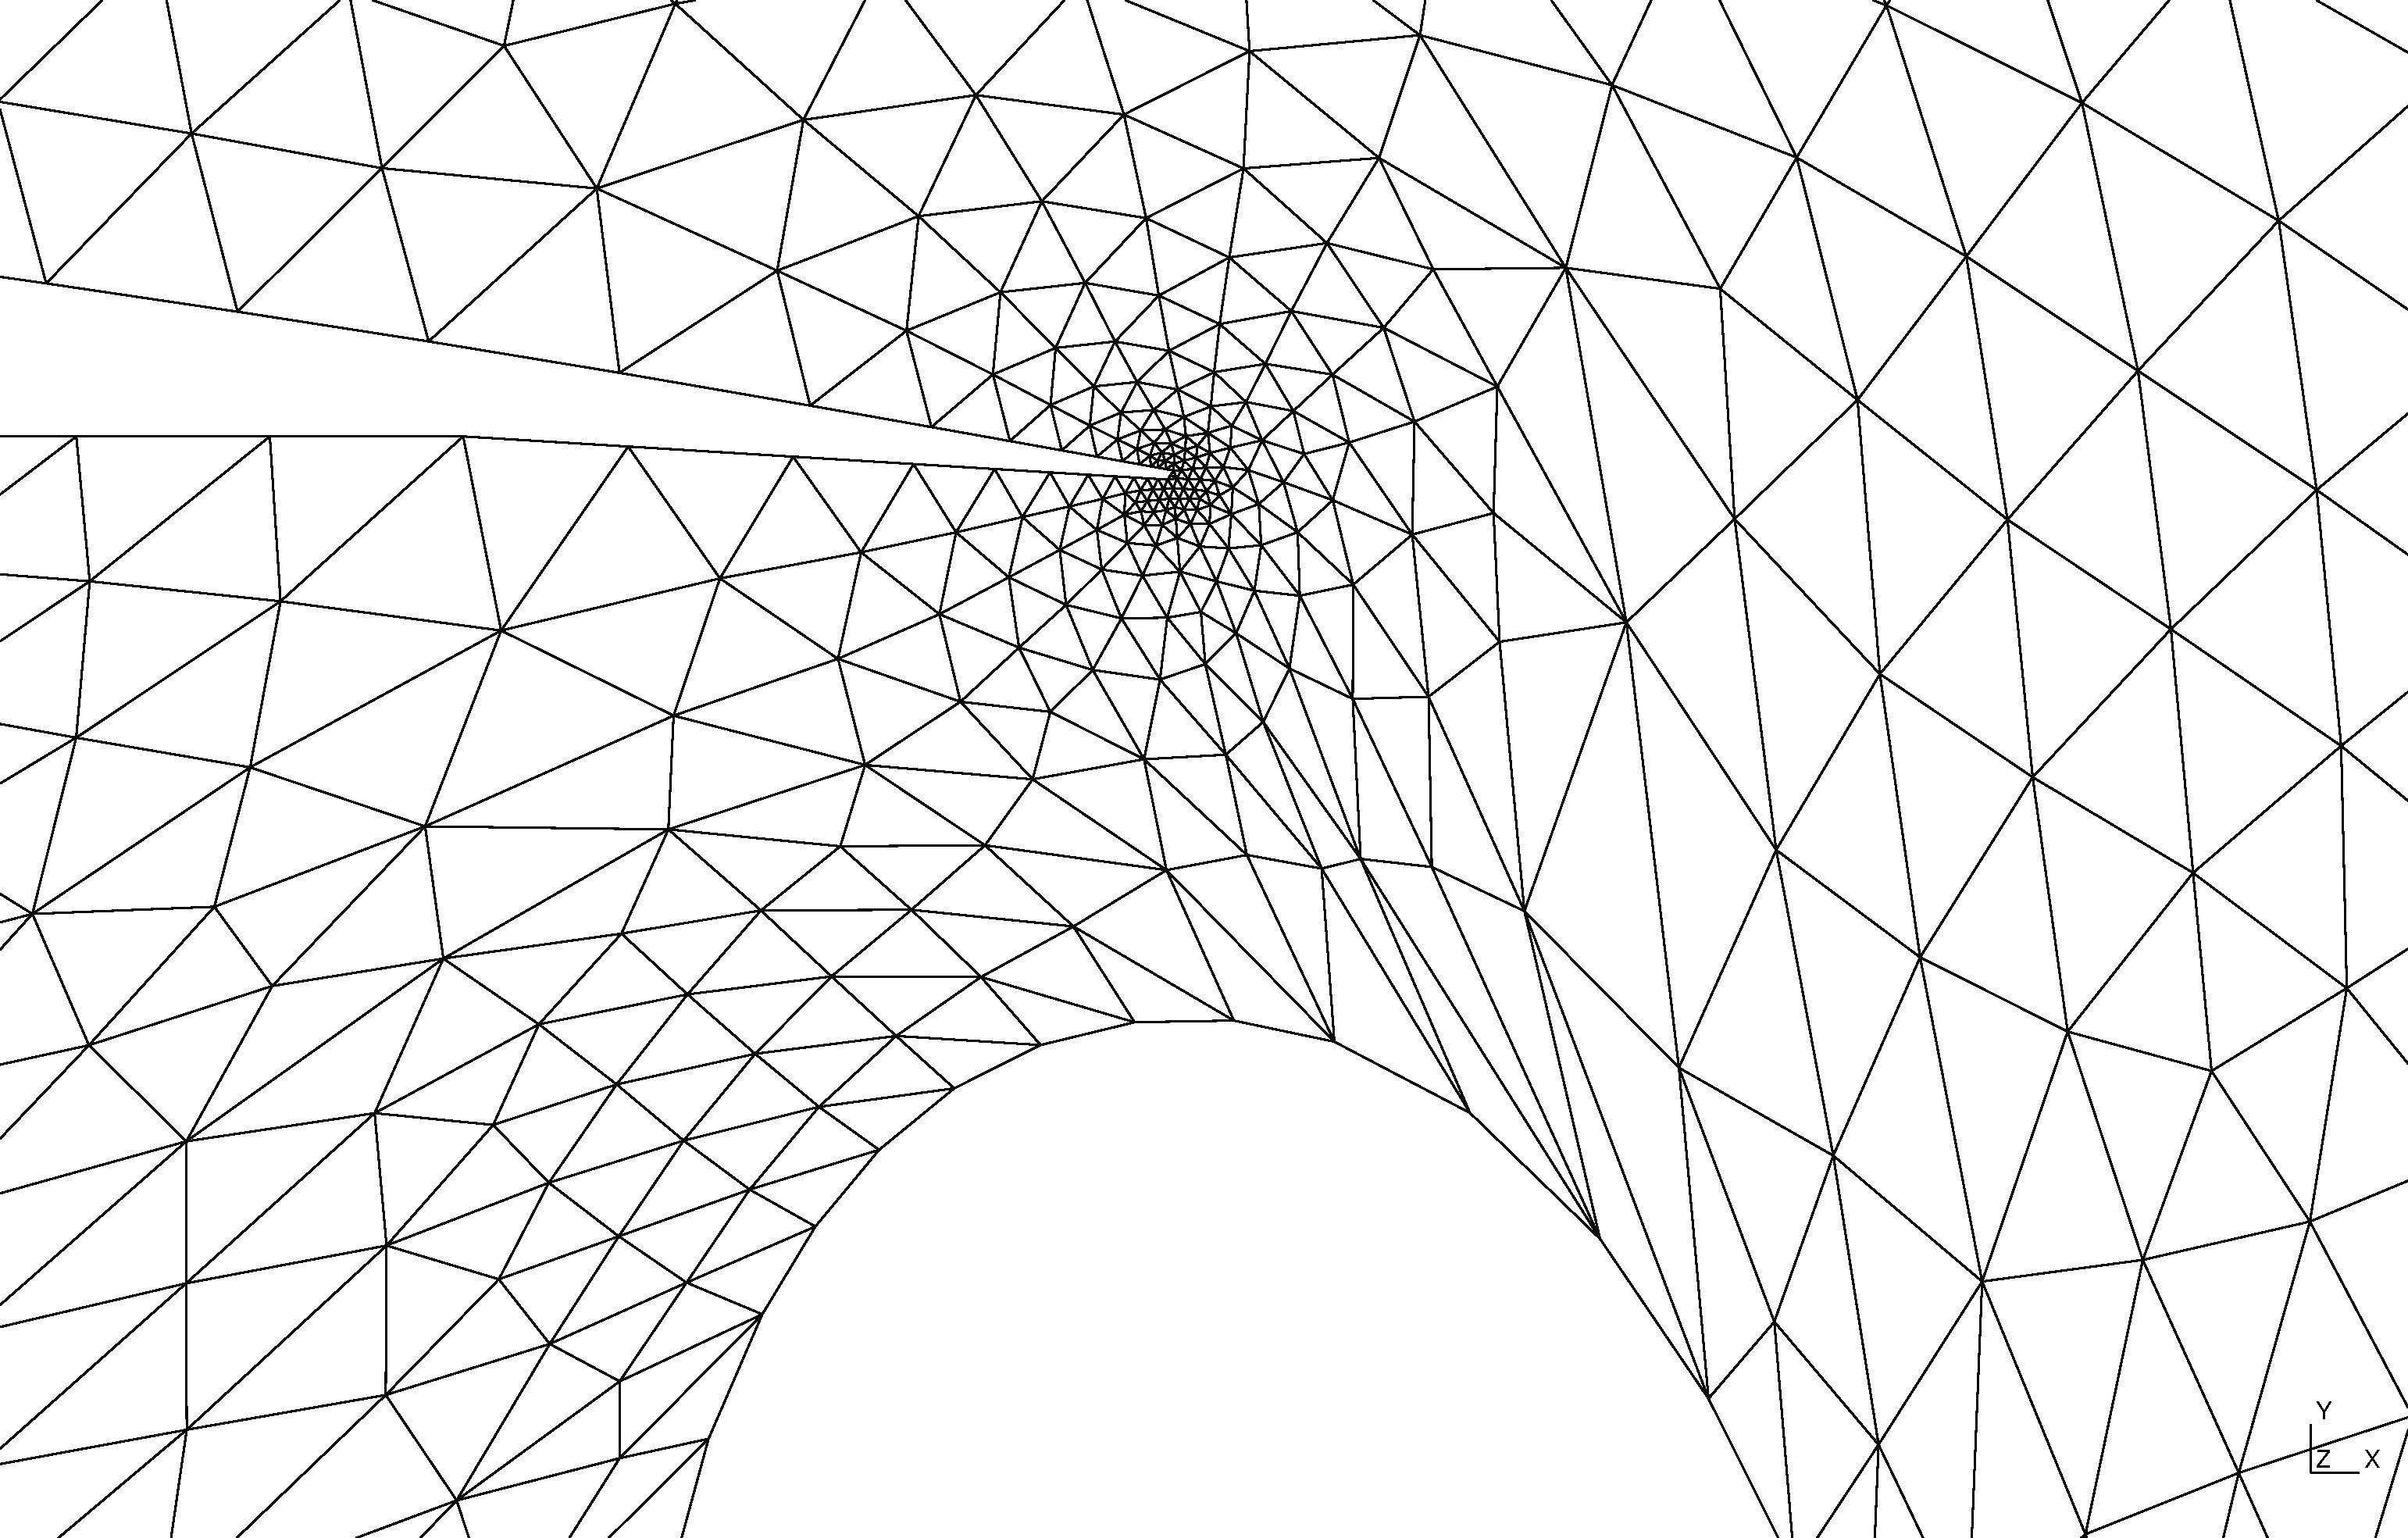
\includegraphics[scale=0.25]{wing60-linelastp1_zoomed}
	\caption{Inviscid 3-component airfoil mesh with 60$^\circ$ rotation of flap by linear elasticity method; zoomed to where the flap meets the wing}
	\label{fig:wing-inviscid-linelastp1-zoomed}
\end{figure}
\begin{figure}
	\centering
	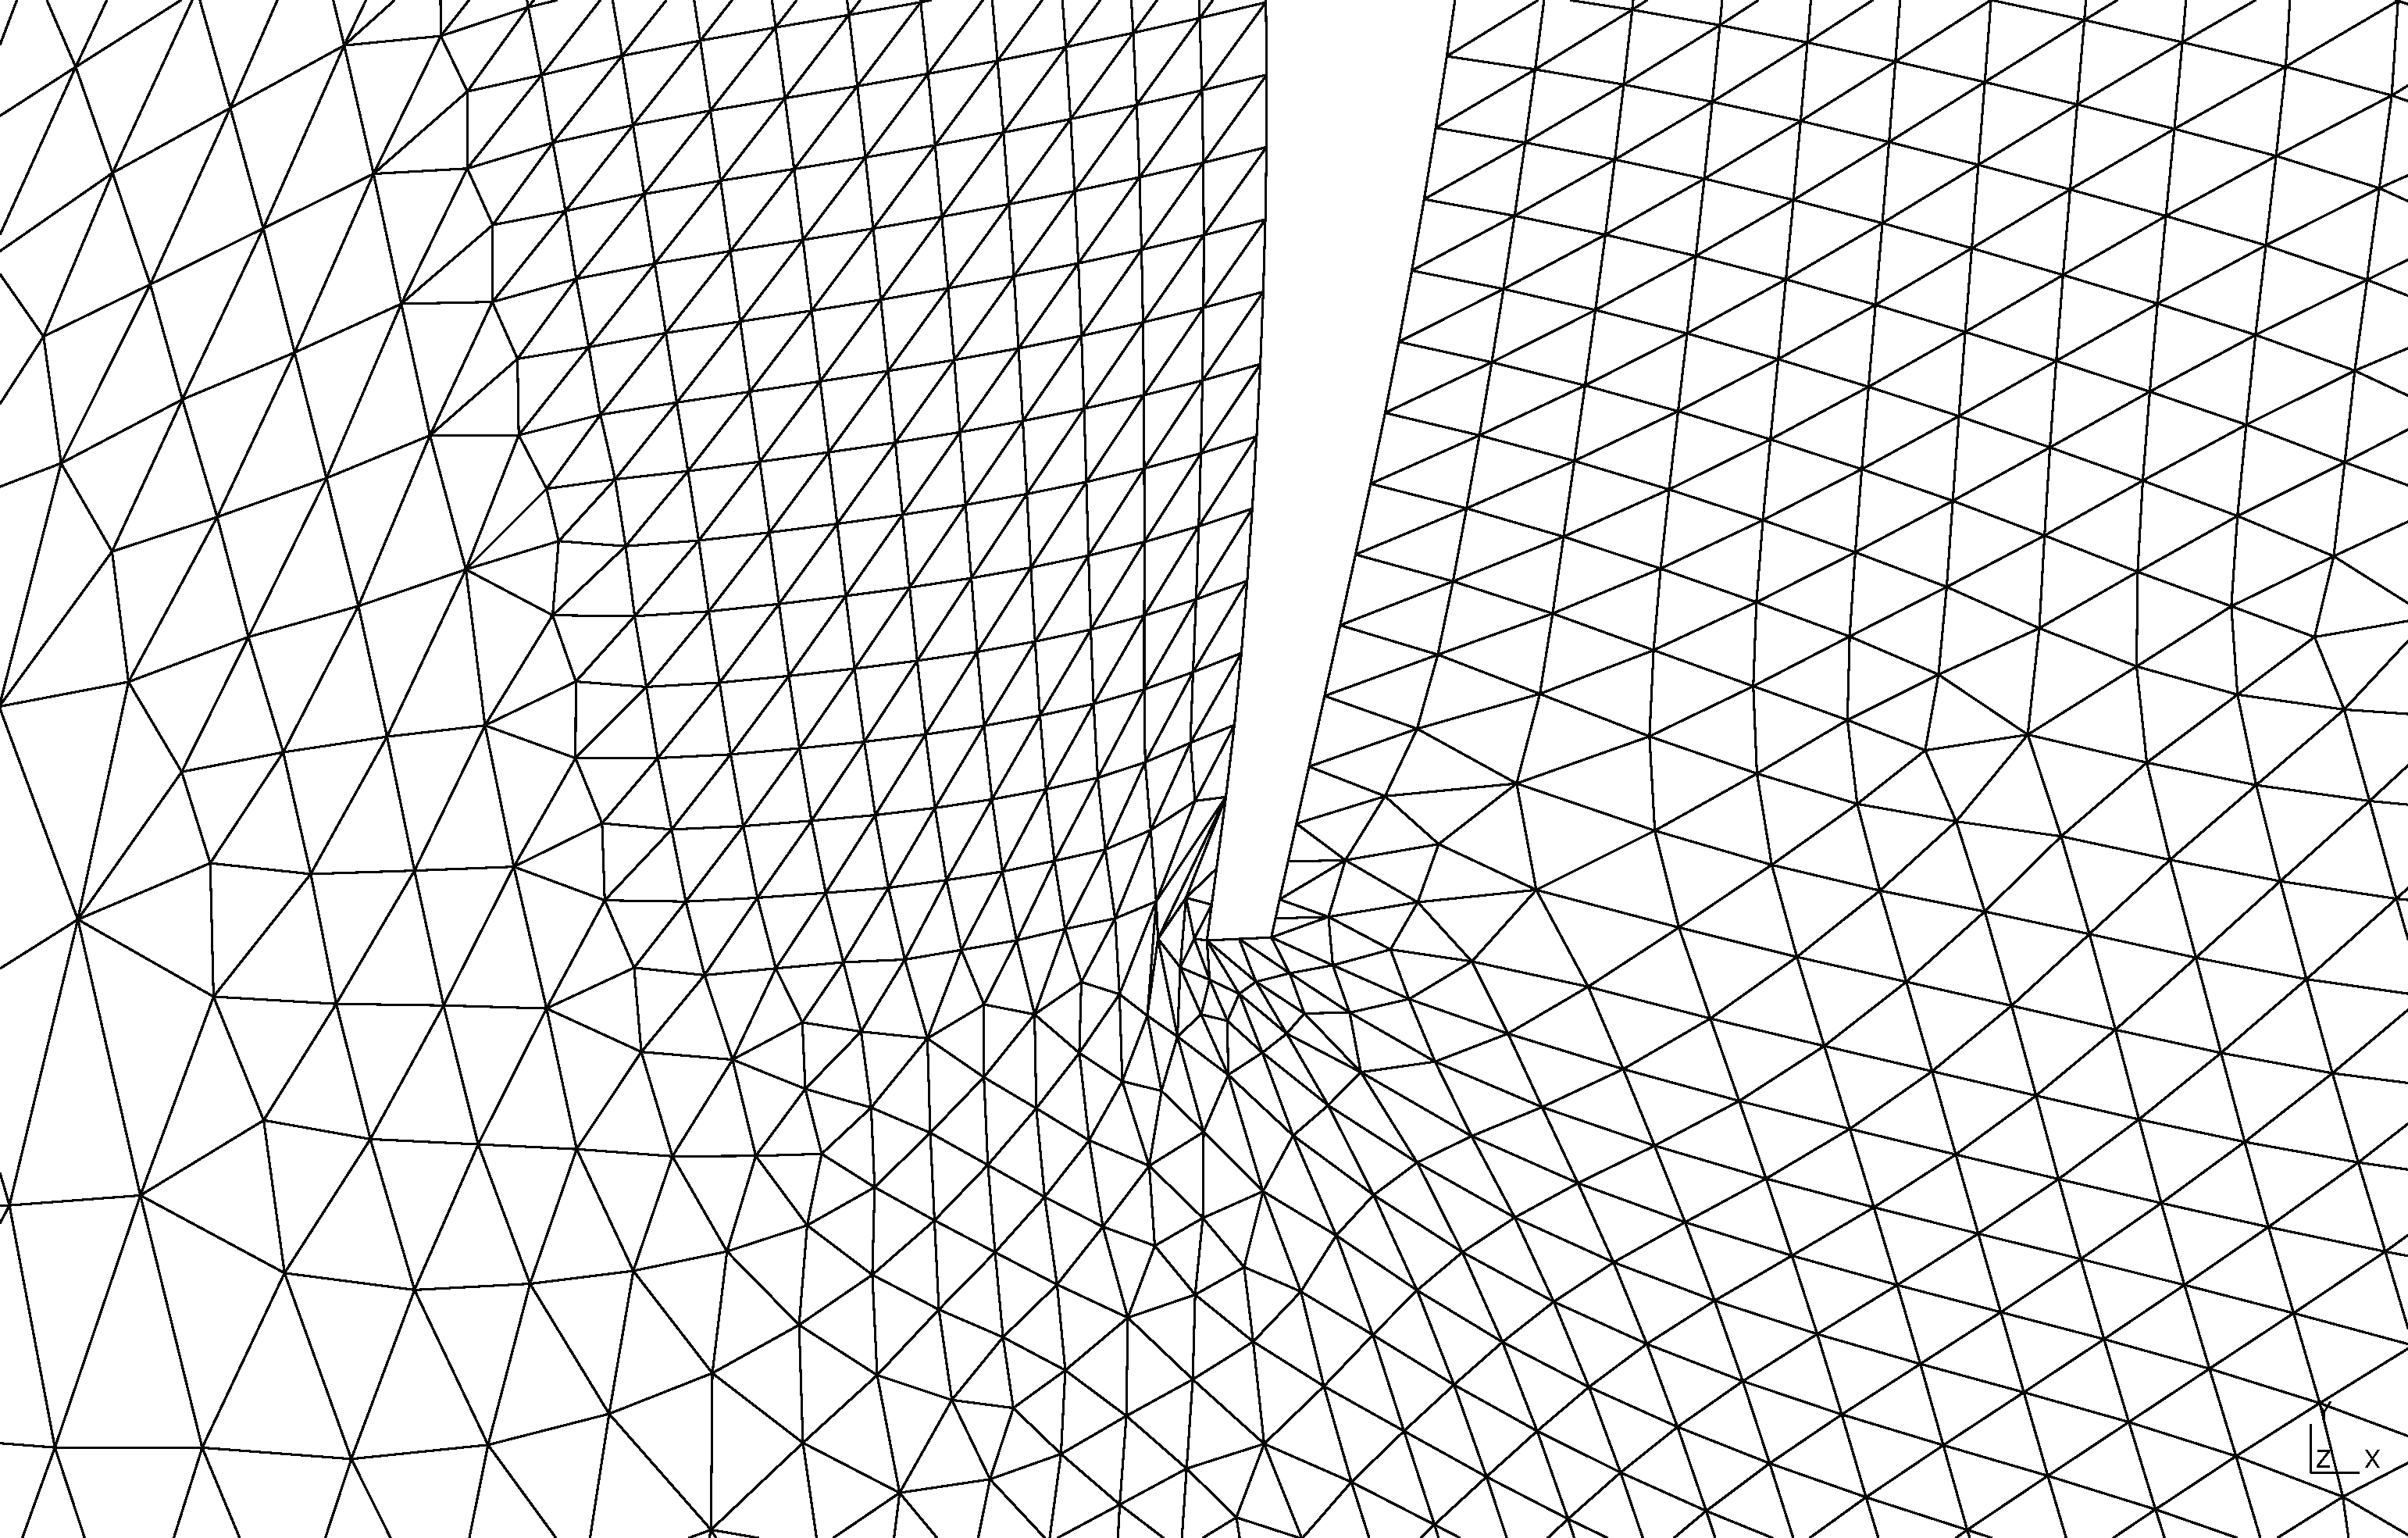
\includegraphics[scale=0.25]{wing60-linelastp1_zoomed2}
	\caption{Inviscid 3-component airfoil mesh with 60$^\circ$ rotation of flap by linear elasticity method, zoomed to the trailing edge of the flap}
	\label{fig:wing-inviscid-linelastp1-zoomed2}
\end{figure}

In figures \ref{fig:wing-inviscid-dg-ms} and \ref{fig:wing-inviscid-dg-ms-zoomed}, we present results with the Delaunay graph mapping (DGM) method. We see that cell quality is severly degraded near the interface between trailing edge of the wing and the flap. The quality of the cells near the trailing edge of the flap is better than the linear elasticity case, however. We remark here that DGM is computationally the most frugal method out of all the ones presented, as we need to solve only 3x3 linear systems after generating a background Delaunay graph, both of which are very fast (sec. \ref{sec:dgm}).

\begin{figure}
	\centering
	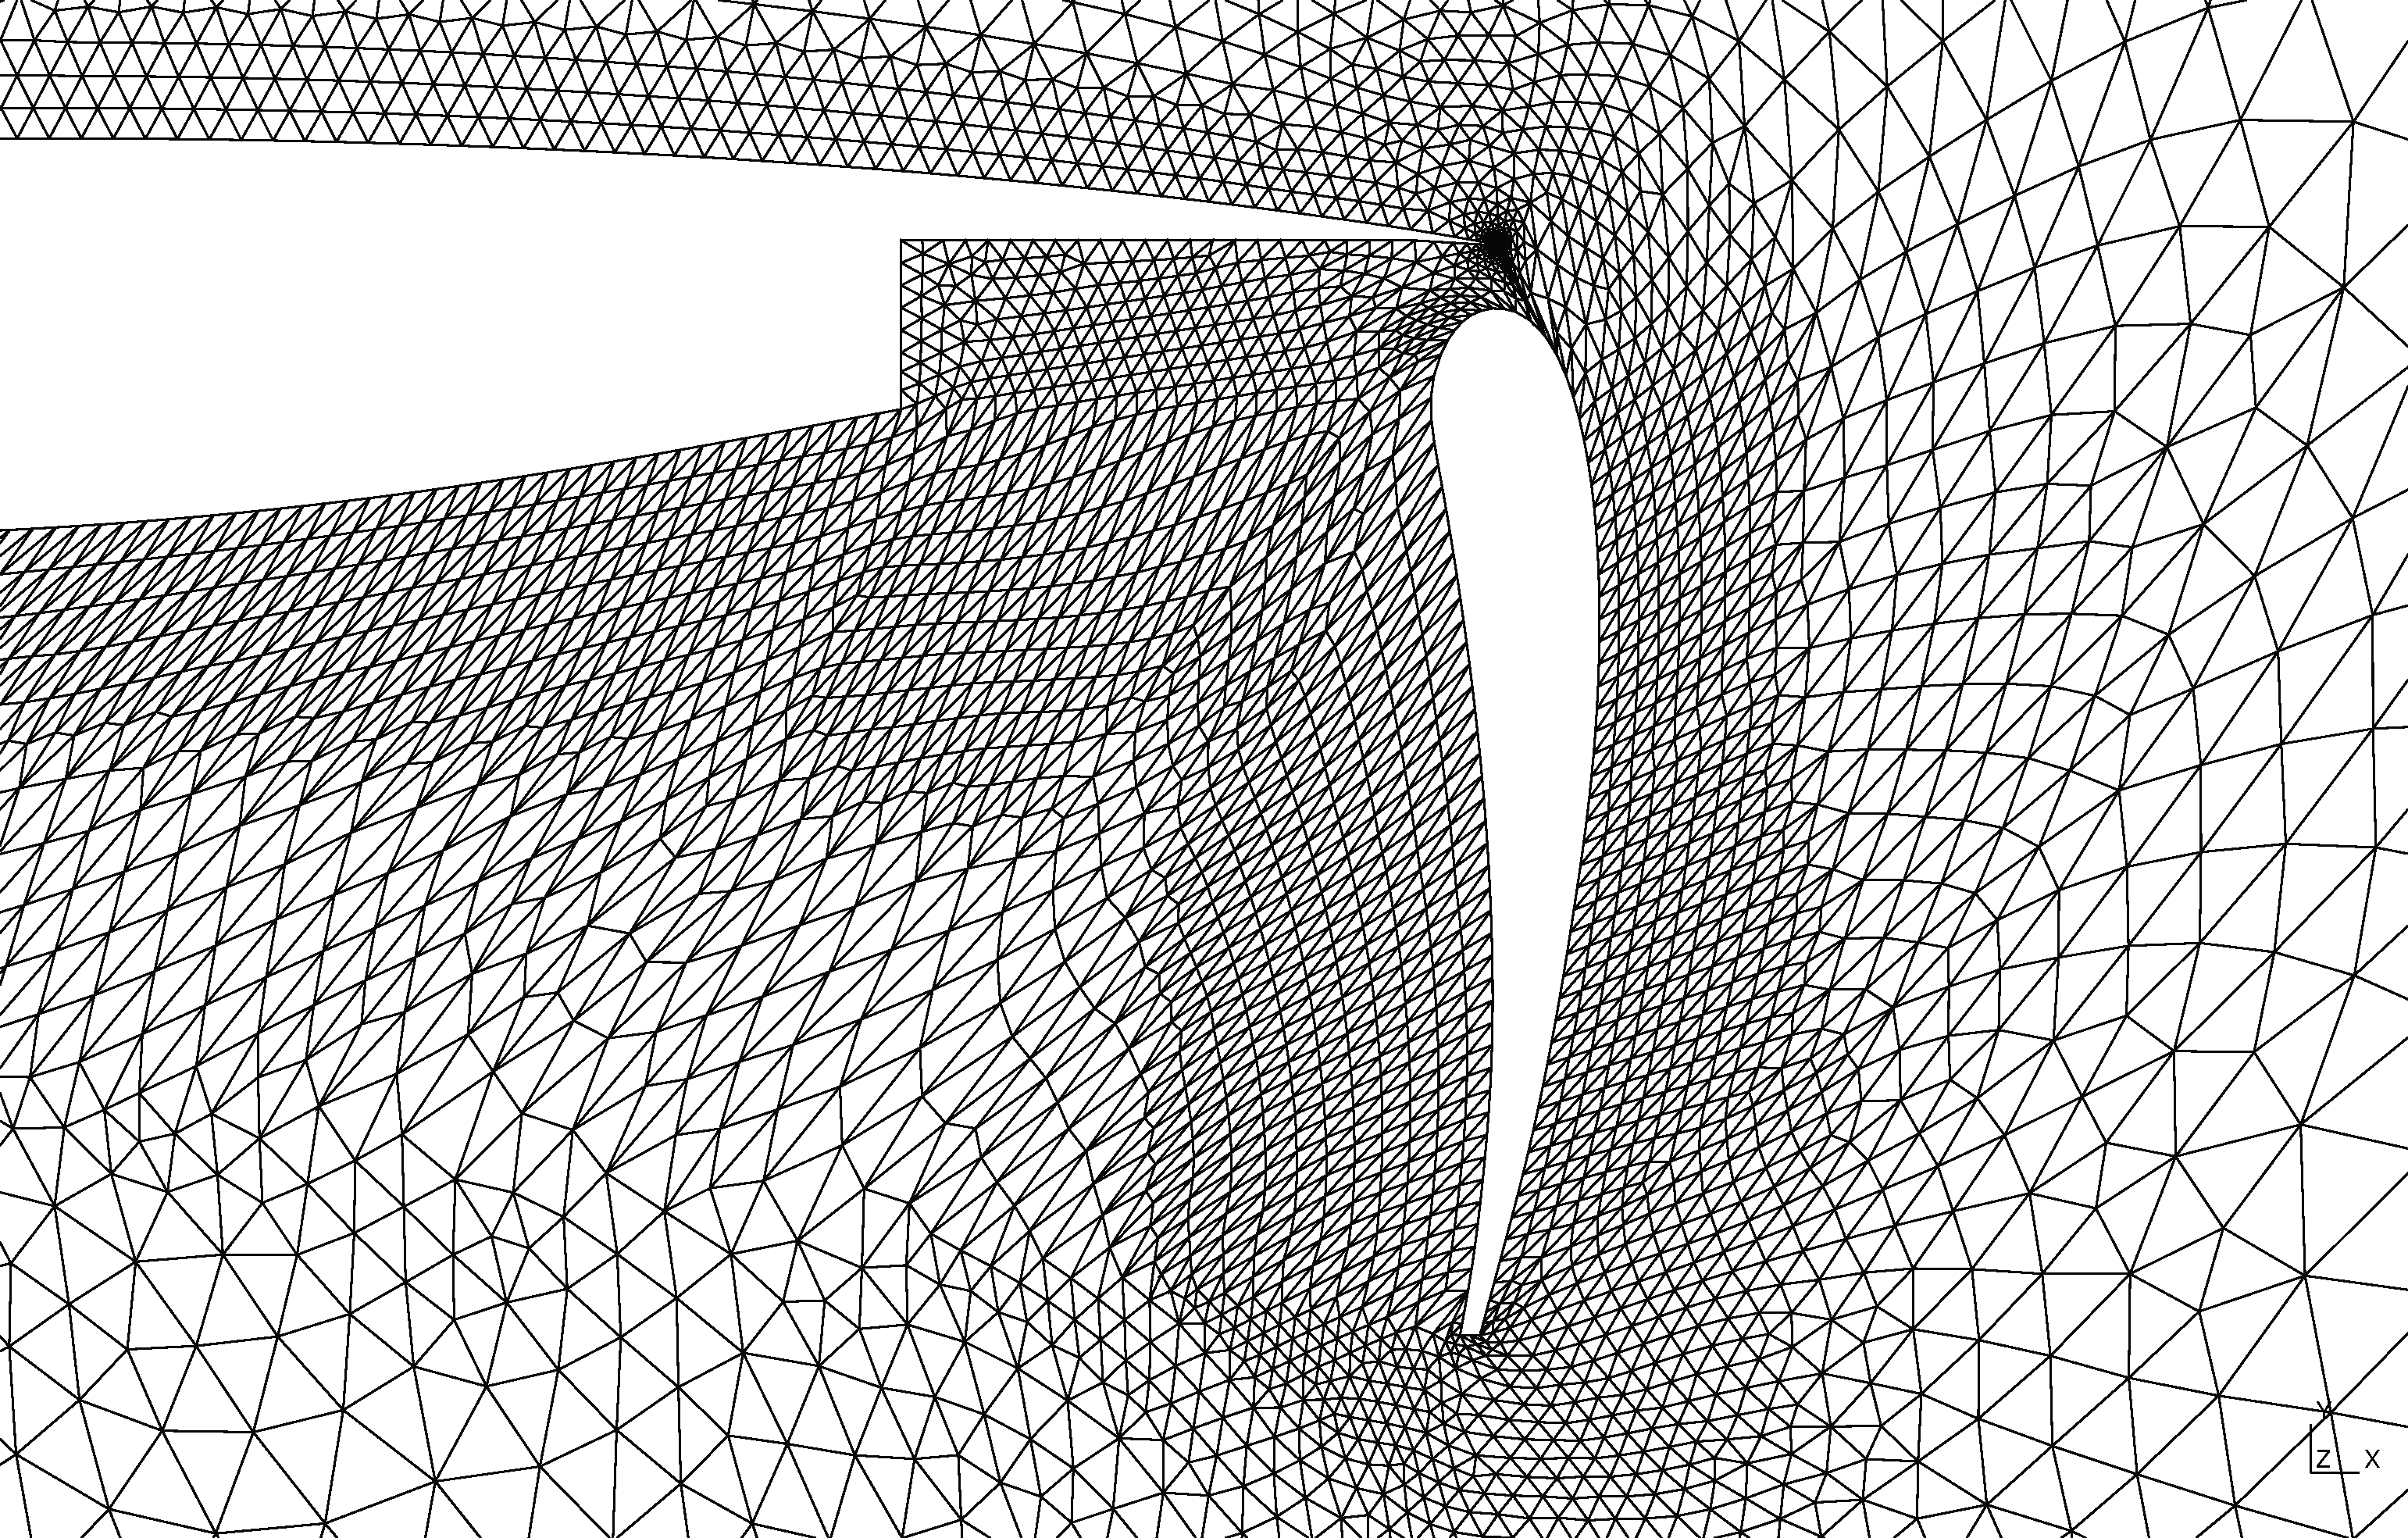
\includegraphics[scale=0.25]{wing60-dg-ms}
	\caption{Inviscid 3-component airfoil mesh with 60$^\circ$ rotation of flap by DGM method}
	\label{fig:wing-inviscid-dg-ms}
\end{figure}
\begin{figure}
	\centering
	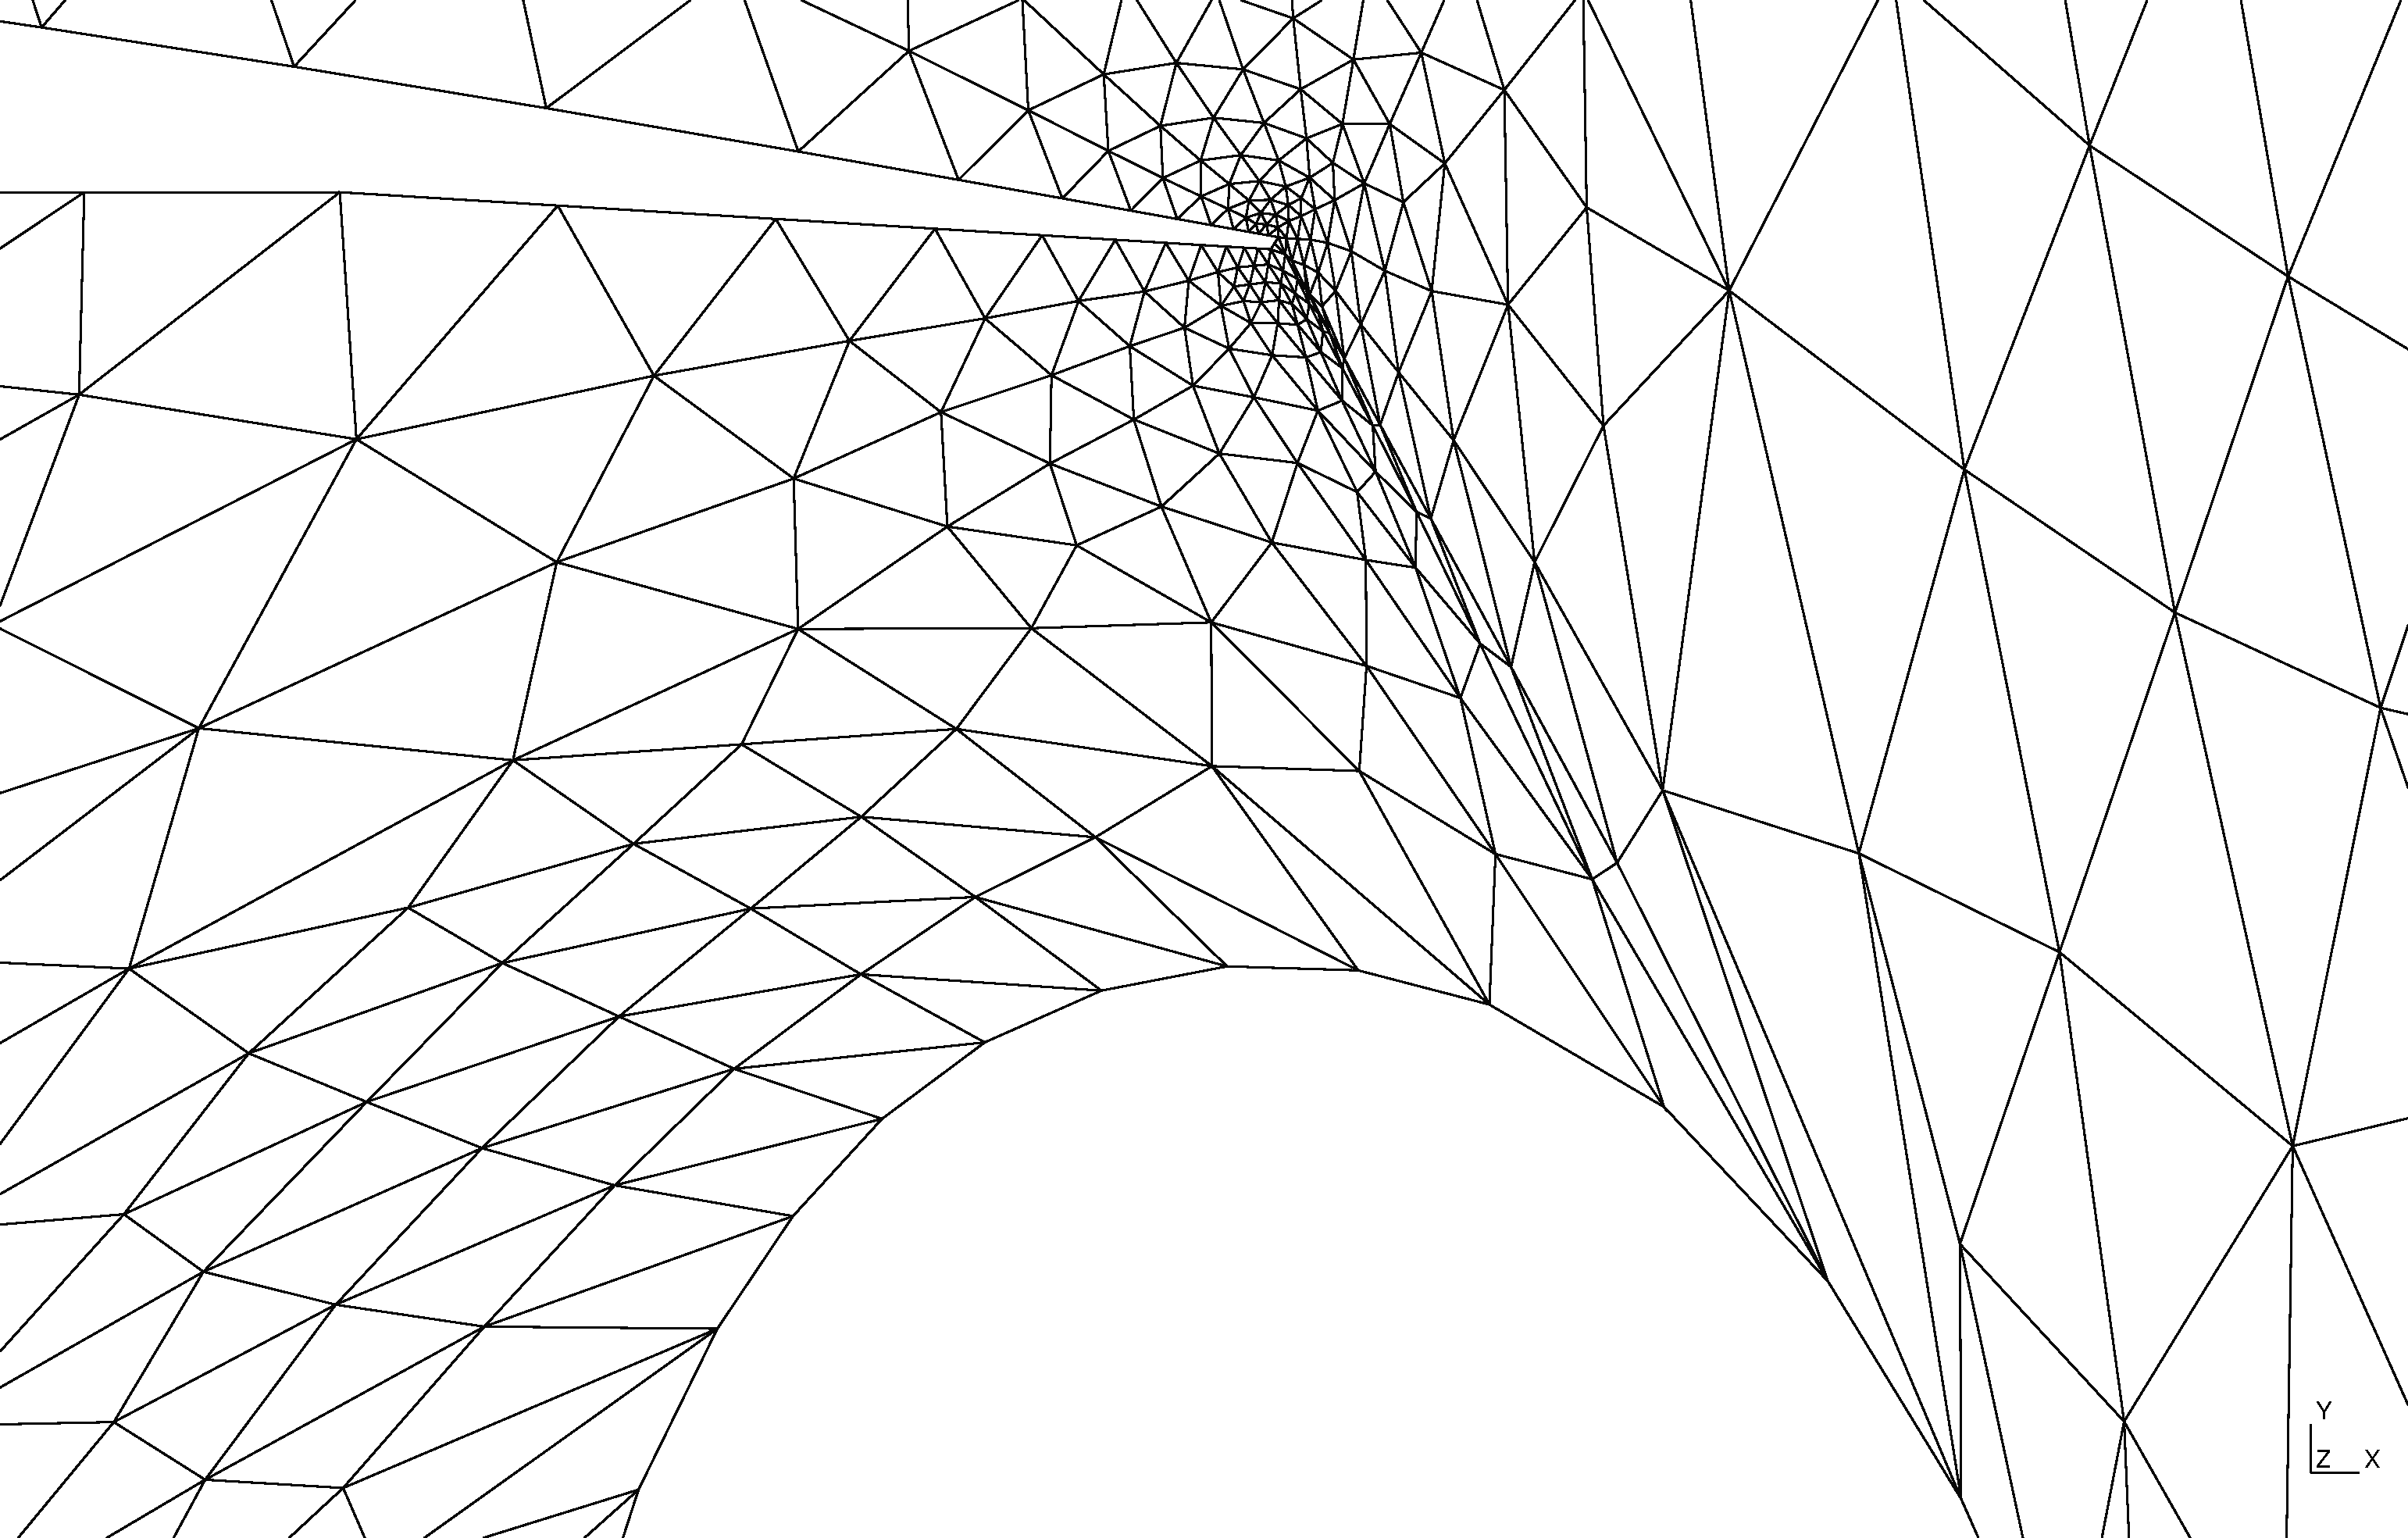
\includegraphics[scale=0.25]{wing60-dg-ms_zoomed}
	\caption{Inviscid 3-component airfoil mesh with 60$^\circ$ rotation of flap by DGM method; zoomed to where the flap meets the wing}
	\label{fig:wing-inviscid-dg-ms-zoomed}
\end{figure}

Finally, we take note of the good qualities of the mesh moved by radial basis function (RBF) interpolation in figures \ref{fig:wing-inviscid-rbf}, \ref{fig:wing-inviscid-rbf-zoomed} and \ref{fig:wing-inviscid-rbf-zoomed2}. We see that mesh quality is not lost to a  great extent anywhere. The support radius is 15.0 units (for reference, the chord length of the wing is approximately 18.3) and the entire movement is carried out in 3 steps.

\begin{figure}
	\centering
	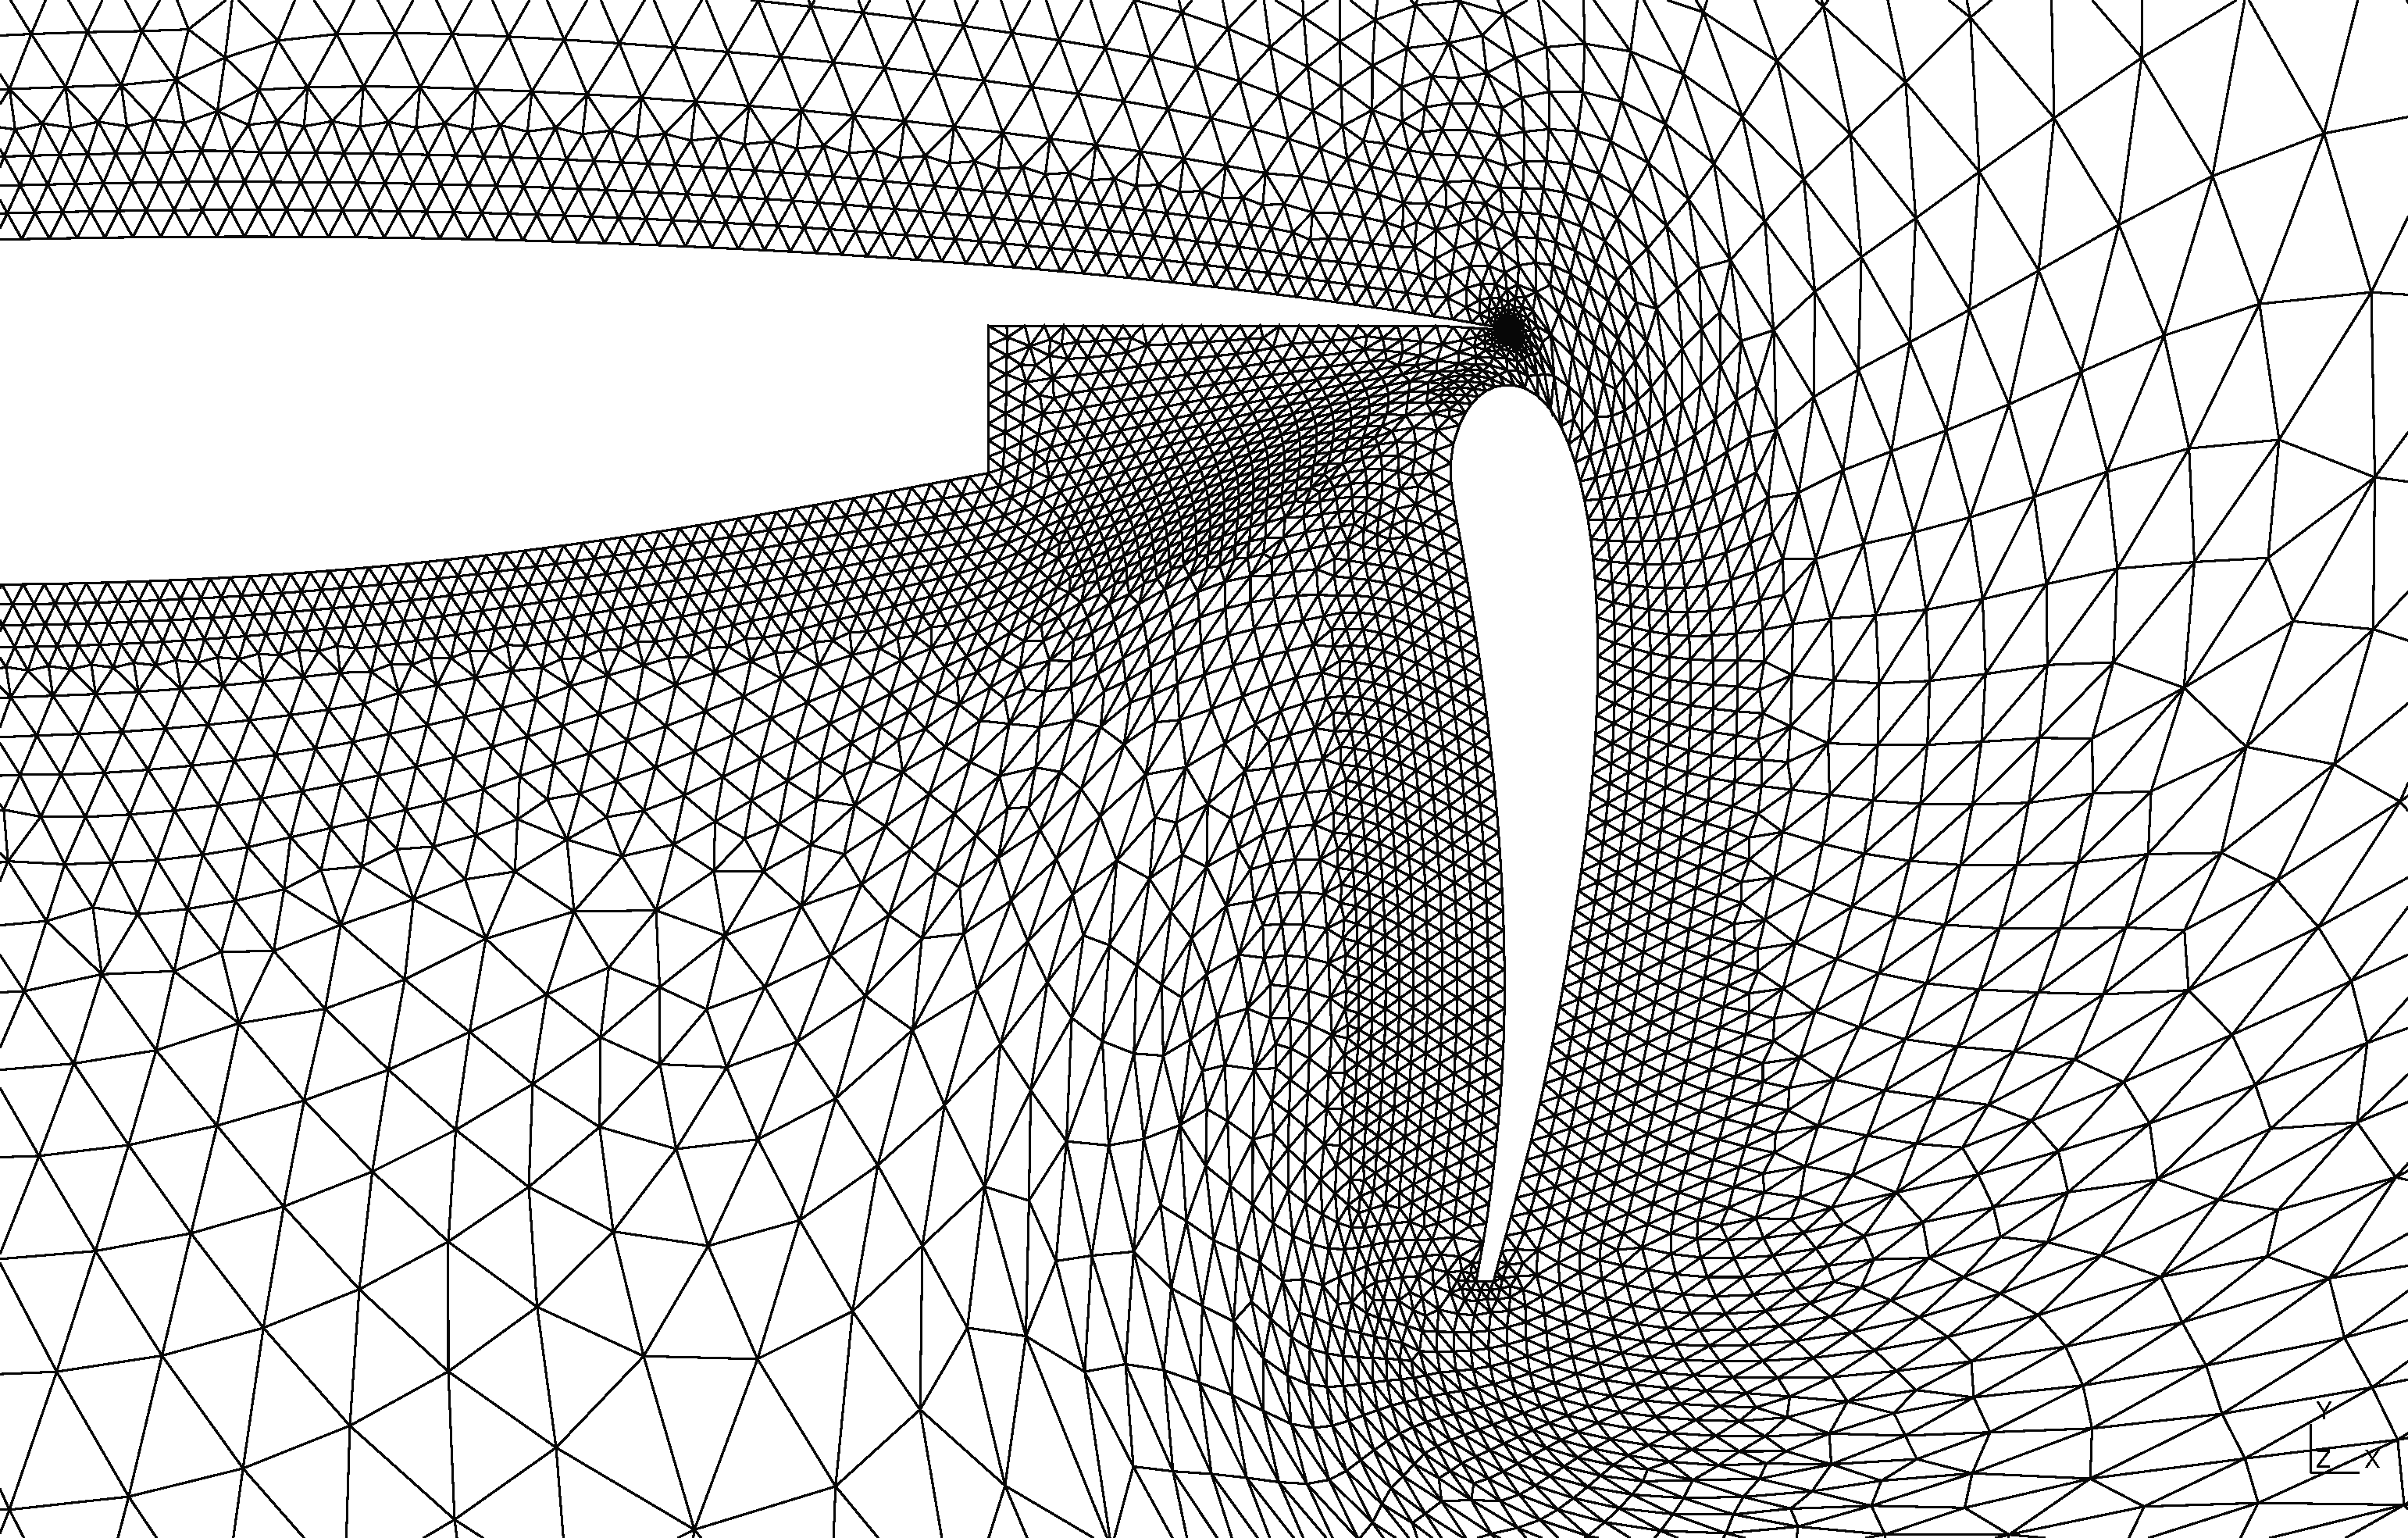
\includegraphics[scale=0.25]{wing60-rbf-sr15-s3}
	\caption{Inviscid 3-component airfoil mesh with 60$^\circ$ rotation of flap by RBF method}
	\label{fig:wing-inviscid-rbf}
\end{figure}
\begin{figure}
	\centering
	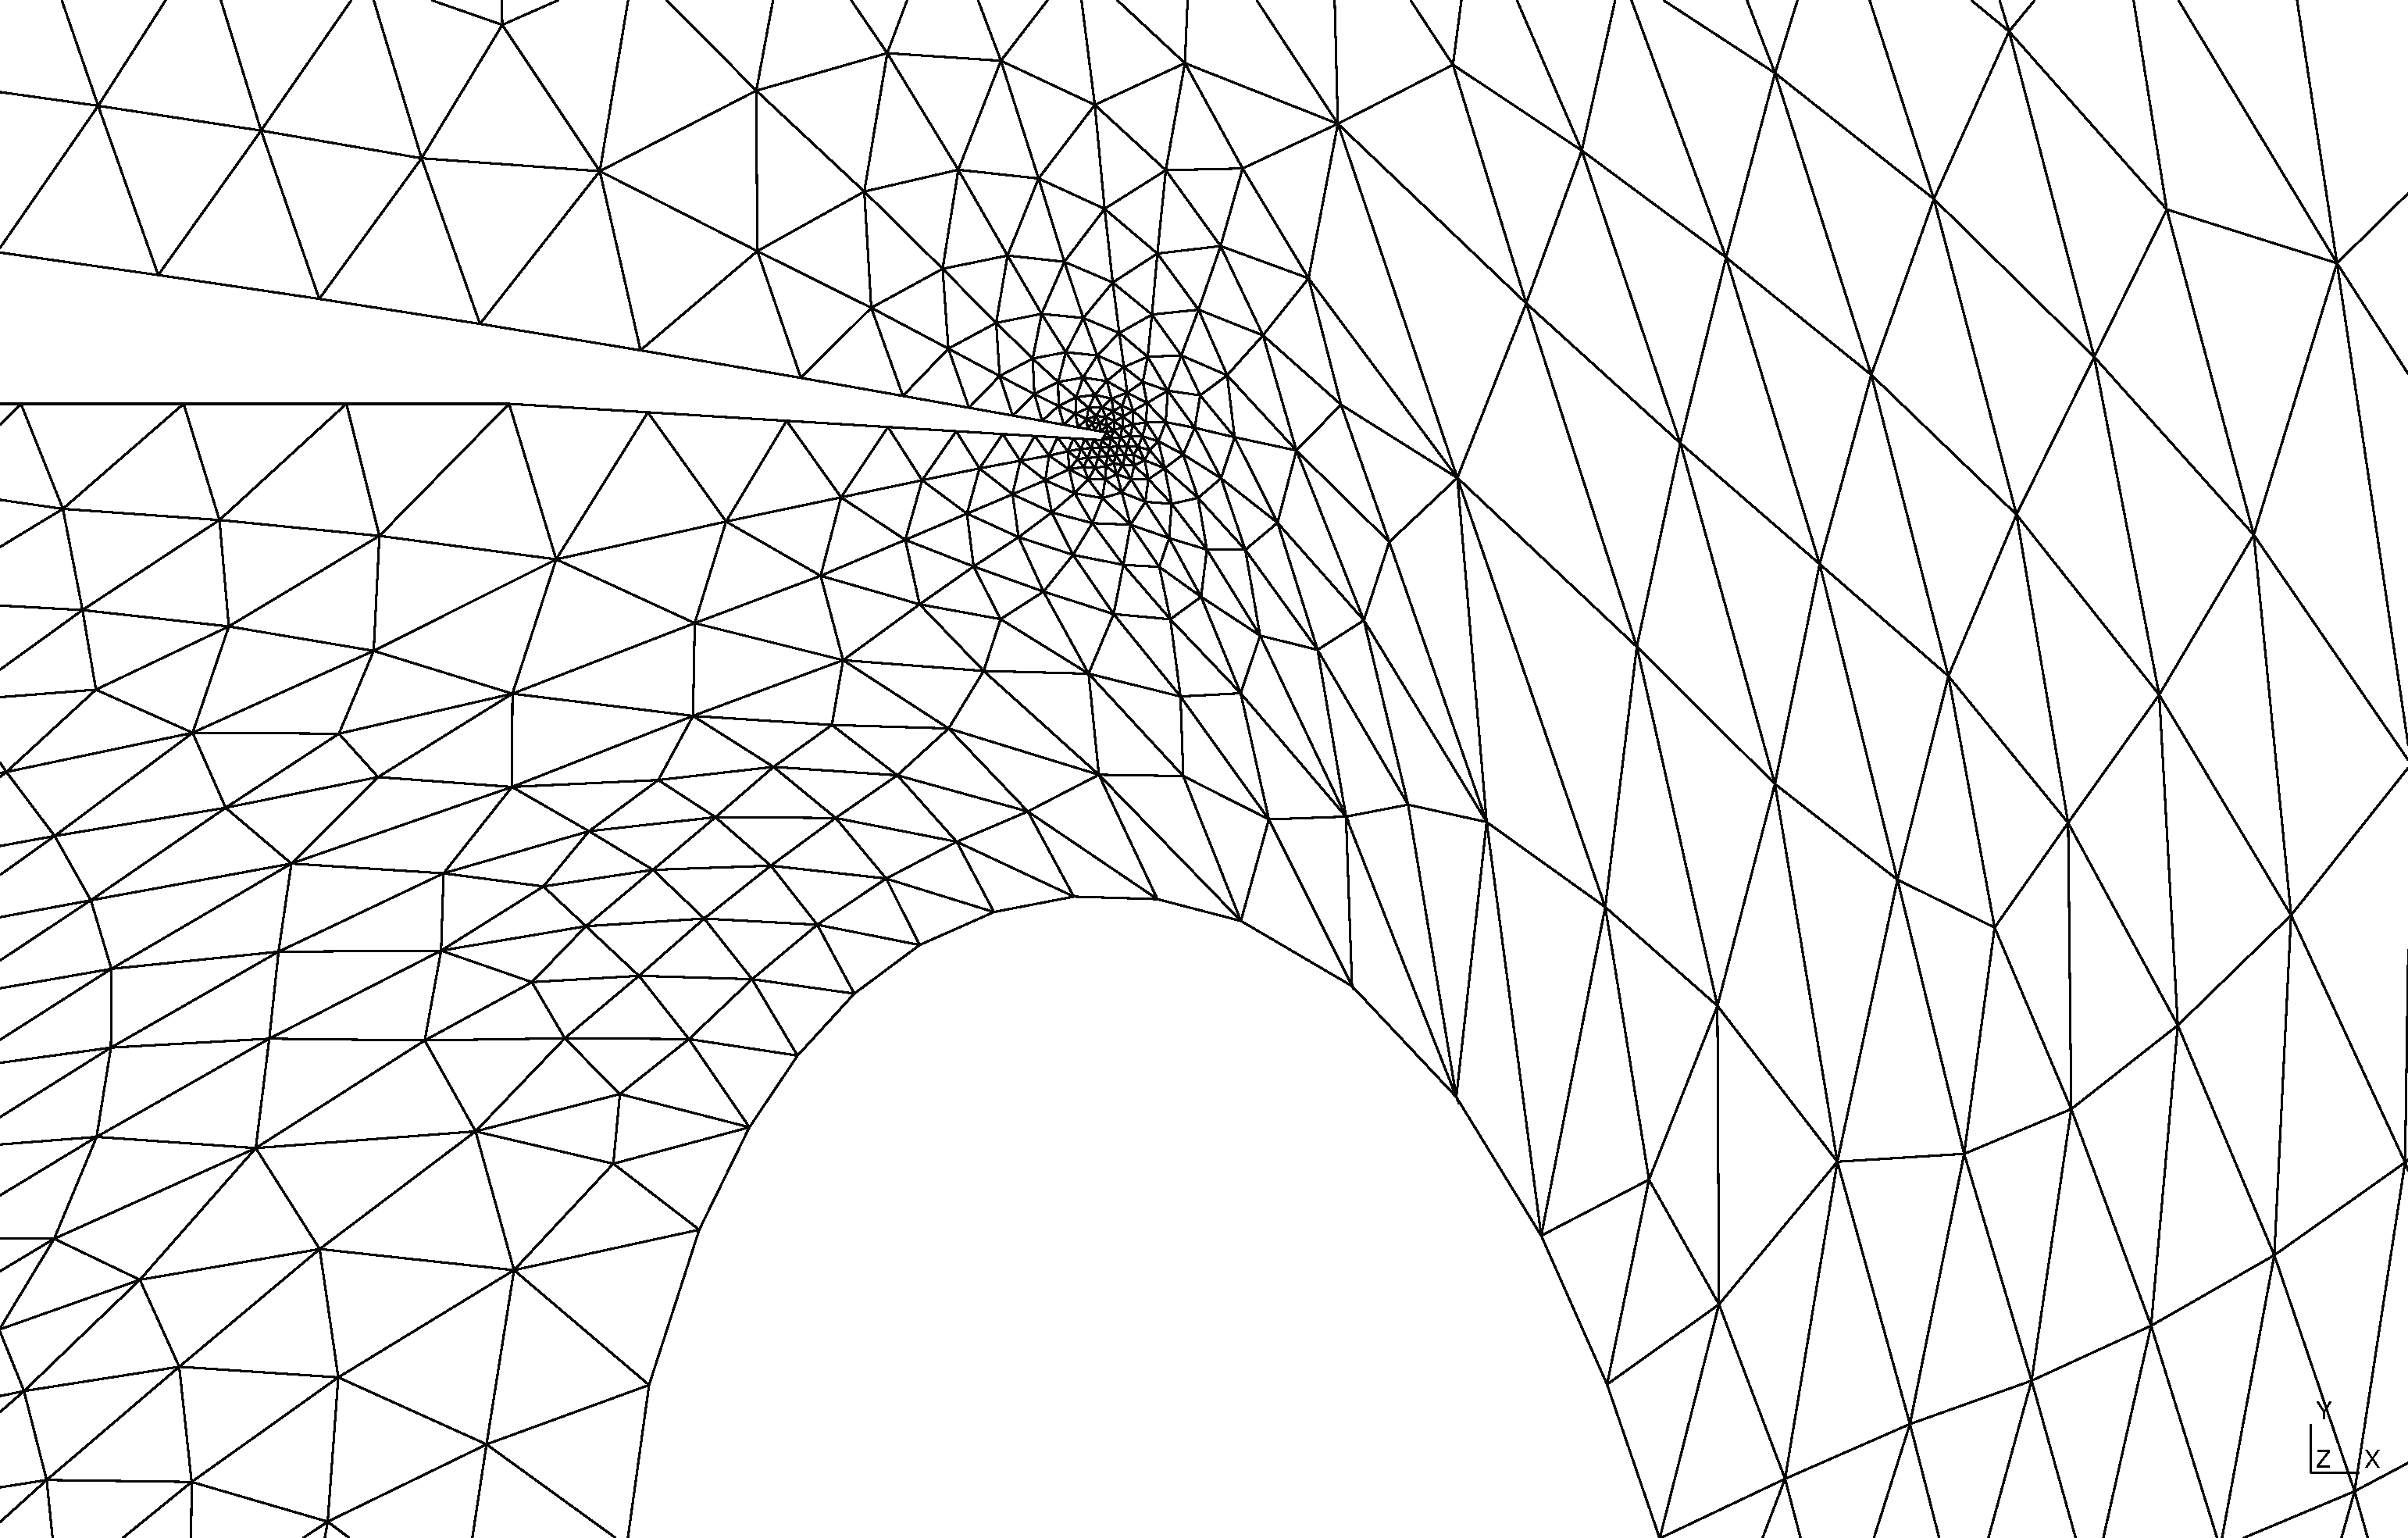
\includegraphics[scale=0.25]{wing60-rbf-sr15-s3_zoomed}
	\caption{Inviscid 3-component airfoil mesh with 60$^\circ$ rotation of flap by RBF method; zoomed to where the flap meets the wing}
	\label{fig:wing-inviscid-rbf-zoomed}
\end{figure}
\begin{figure}
	\centering
	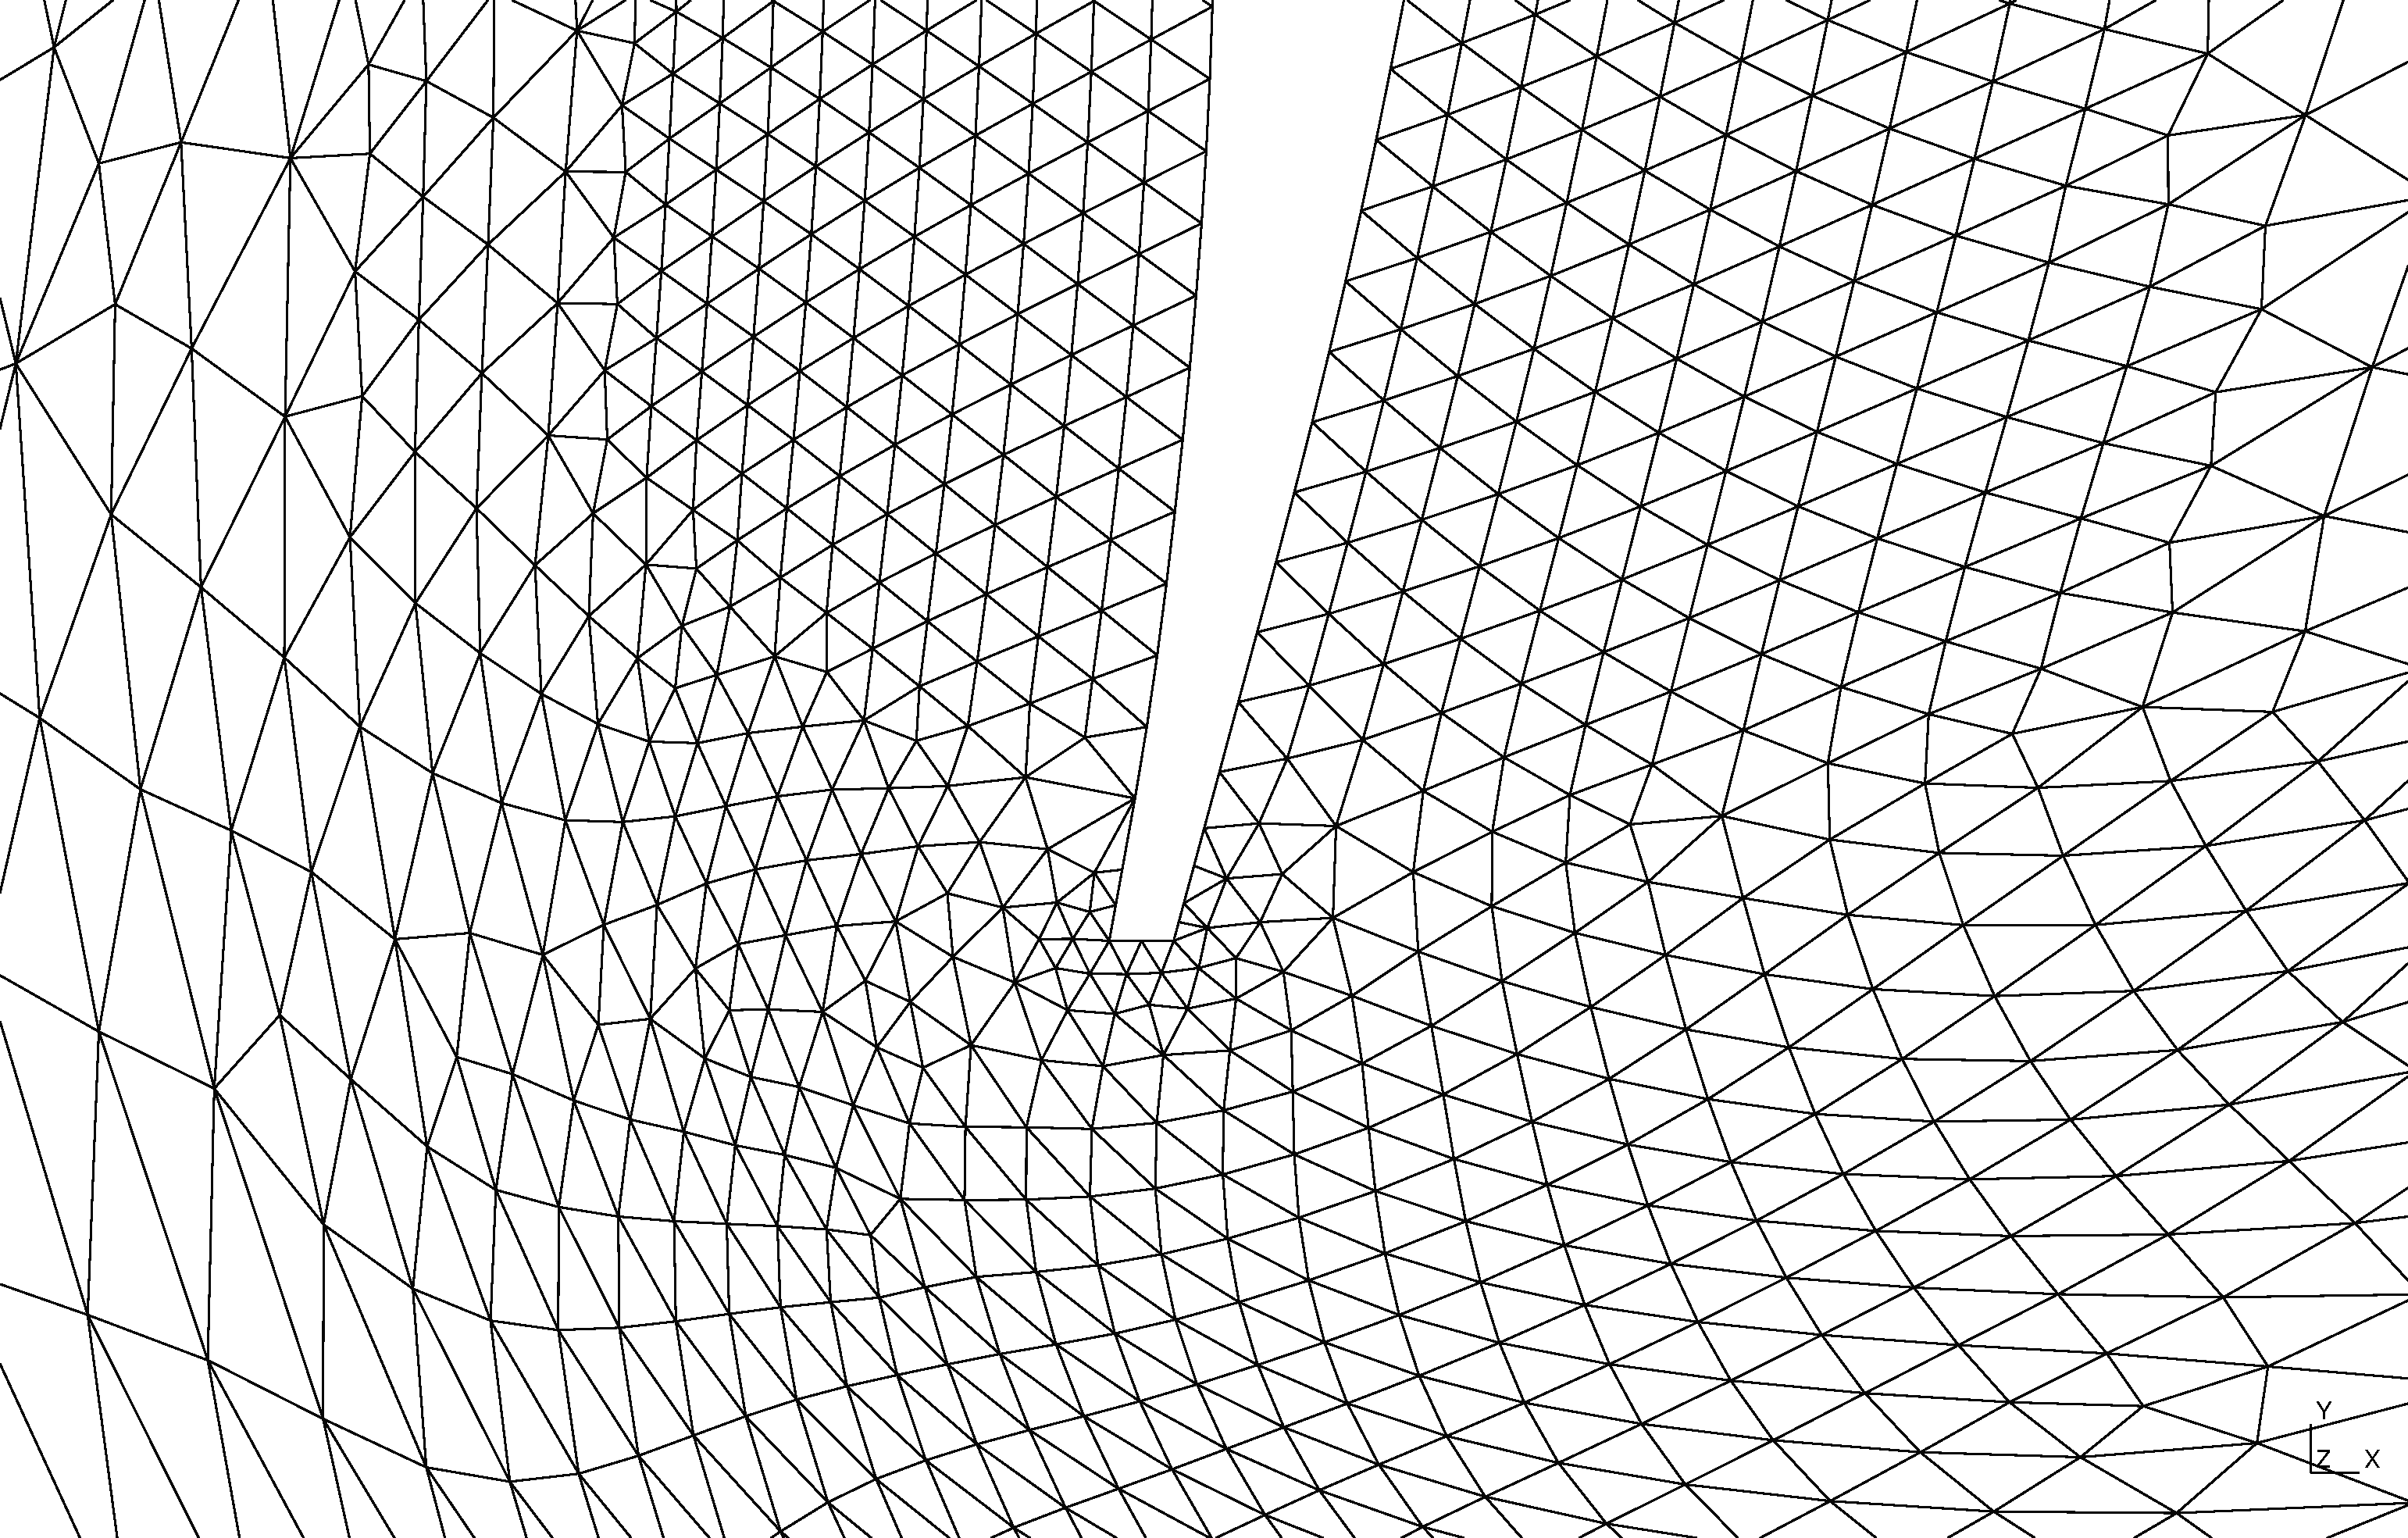
\includegraphics[scale=0.25]{wing60-rbf-sr15-s3_zoomed2}
	\caption{Inviscid 3-component airfoil mesh with 60$^\circ$ rotation of flap by RBF method, zoomed to the trailing edge of the flap}
	\label{fig:wing-inviscid-rbf-zoomed2}
\end{figure}
 
\FloatBarrier

 We present a case of rotation of an interior object inside a far-field boundary using interpolation methods on a quadrilateral mesh. The skew metric has been computed for this case. We show results for a 60-degree rotation in case of DGM (fig. \ref{fig:qin-60-dgm}), RBF (fig. \ref{fig:qin-60-rbf}) and DG-RBF2 (fig. \ref{fig:qin-60-dgrbf2}) methods. Note that DGRBF2 refers to the interpolation of rotation angles by DGRBF. The case has been referred from Wang \emph{et. al.} \cite{mm:dgrbf}. Figure \ref{fig:qin-orig} shows the un-deformed mesh.
 
 \begin{figure}
 	\centering
 	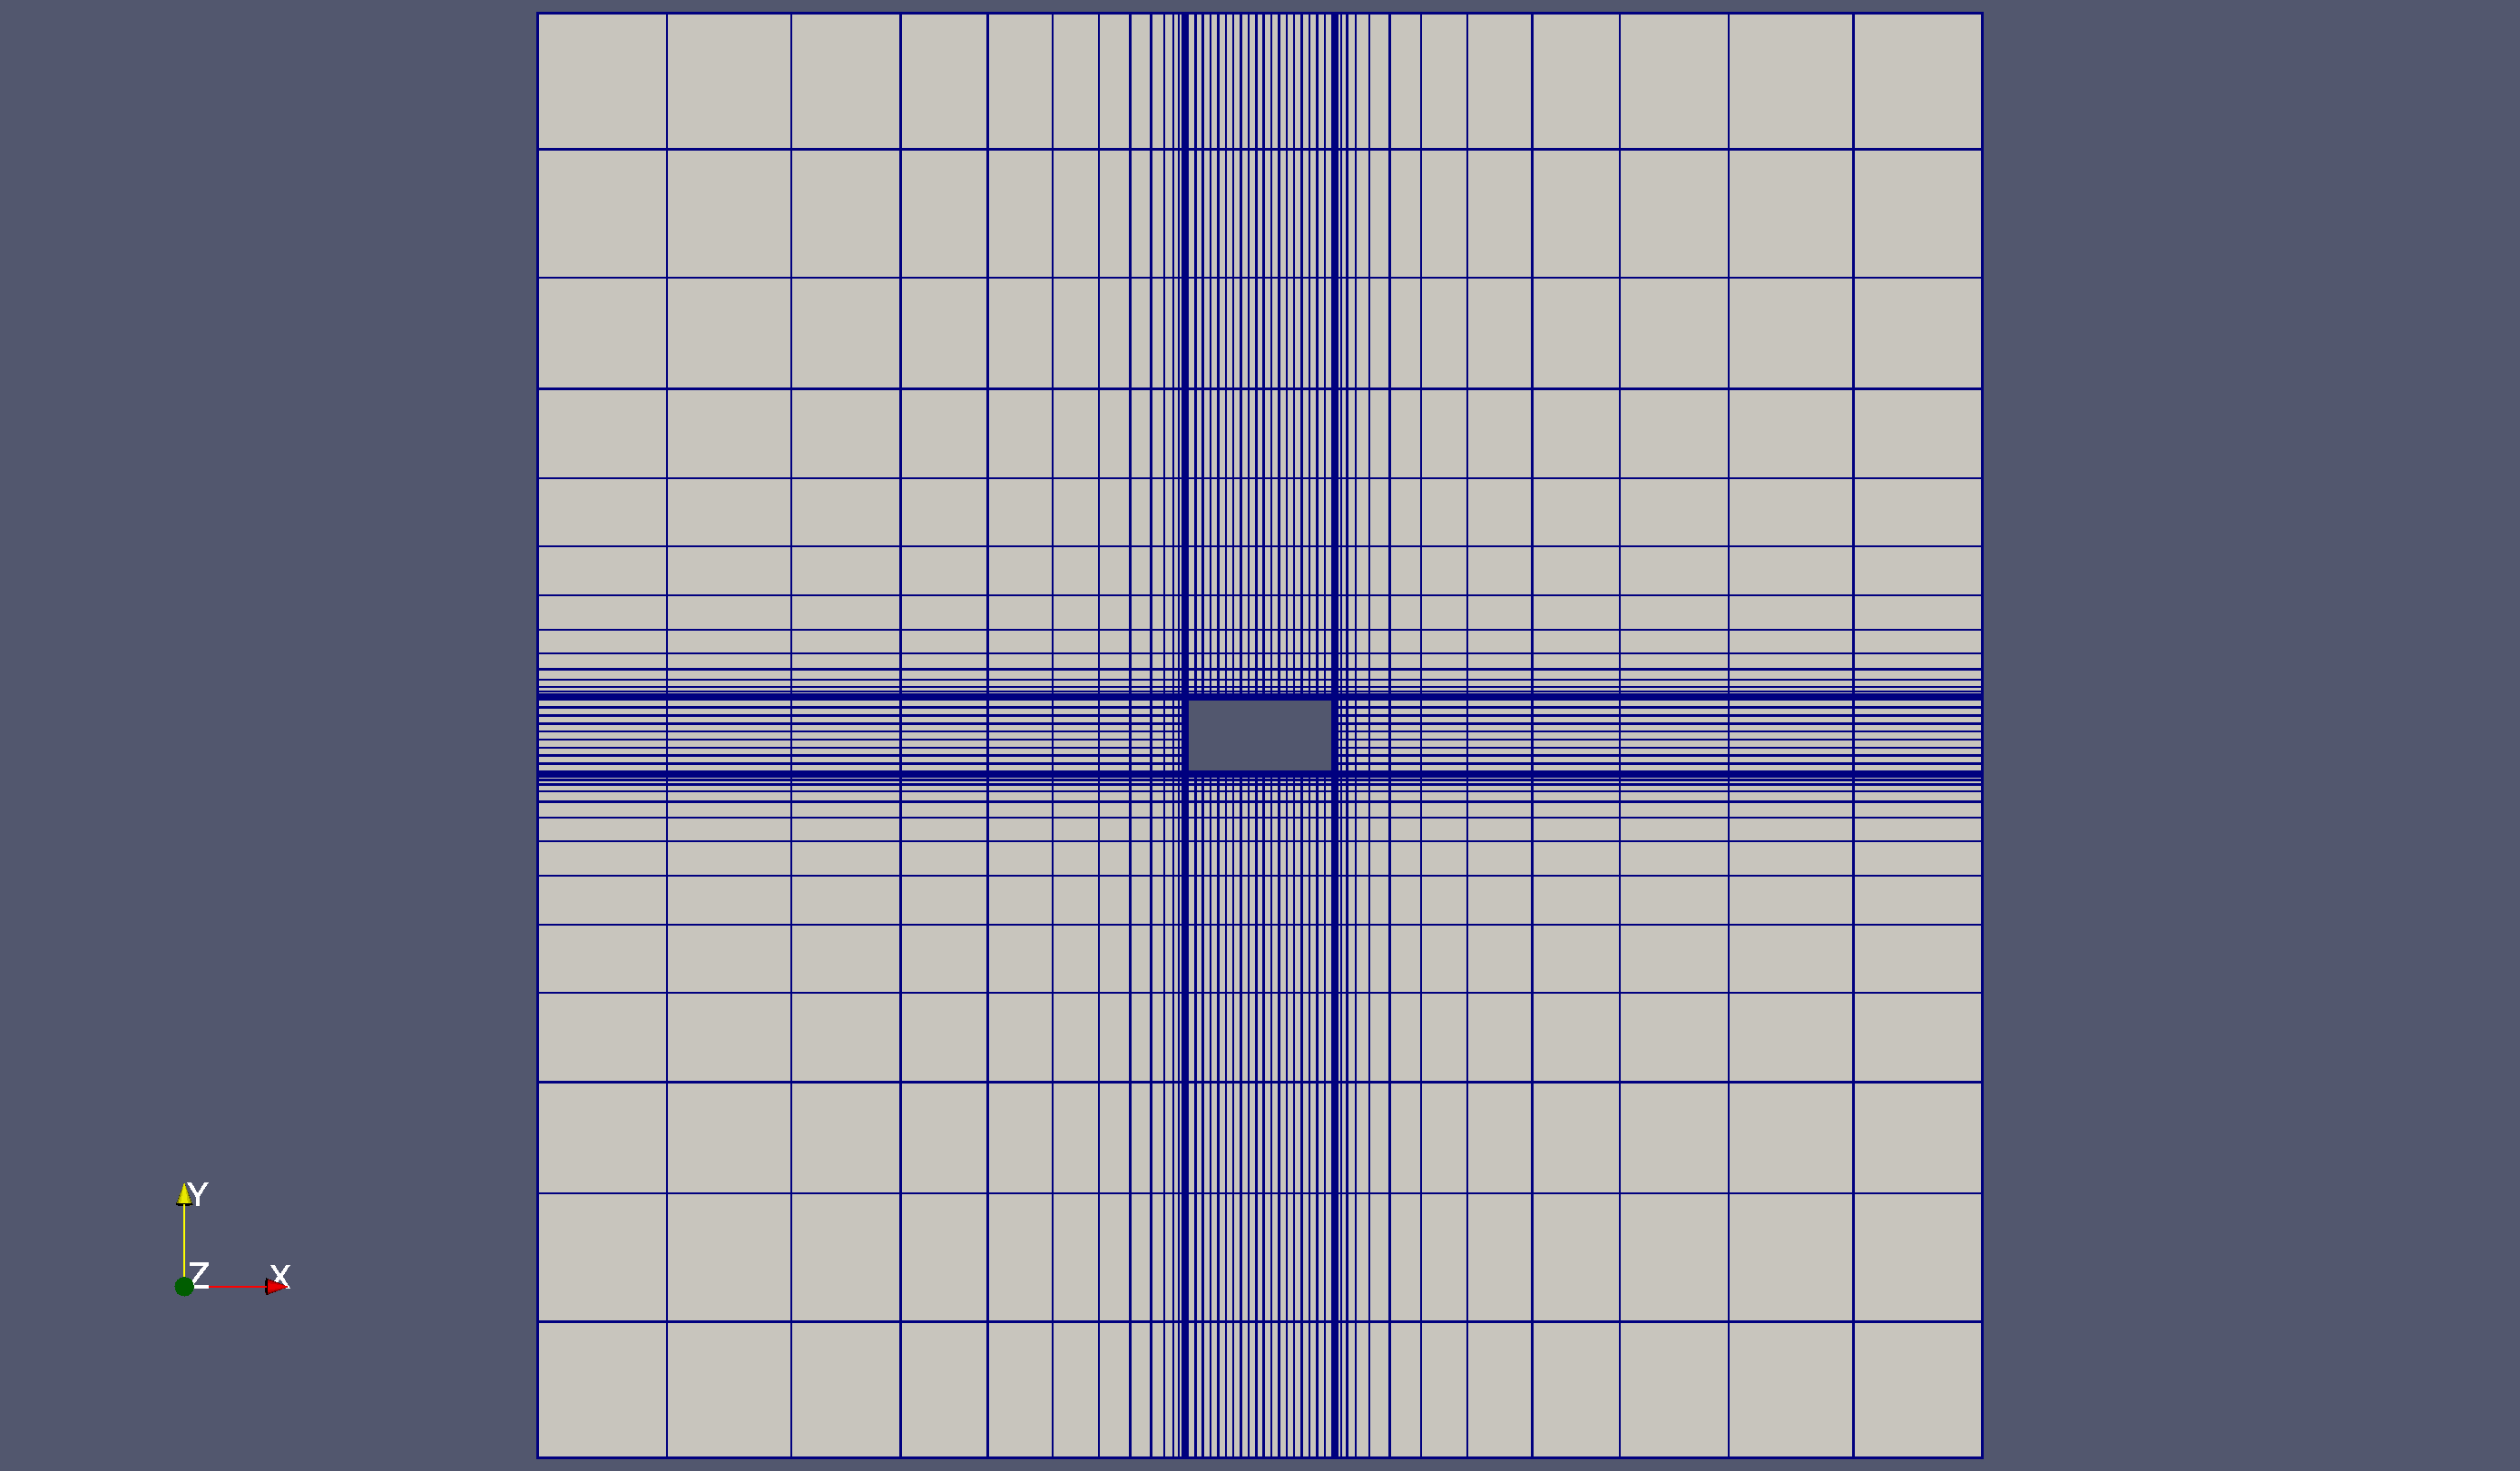
\includegraphics[scale=0.25]{qin-orig-mesh.pdf}
 	\caption{Original mesh}
 	\label{fig:qin-orig}
 \end{figure}
 
 \begin{figure}
 	\centering
 	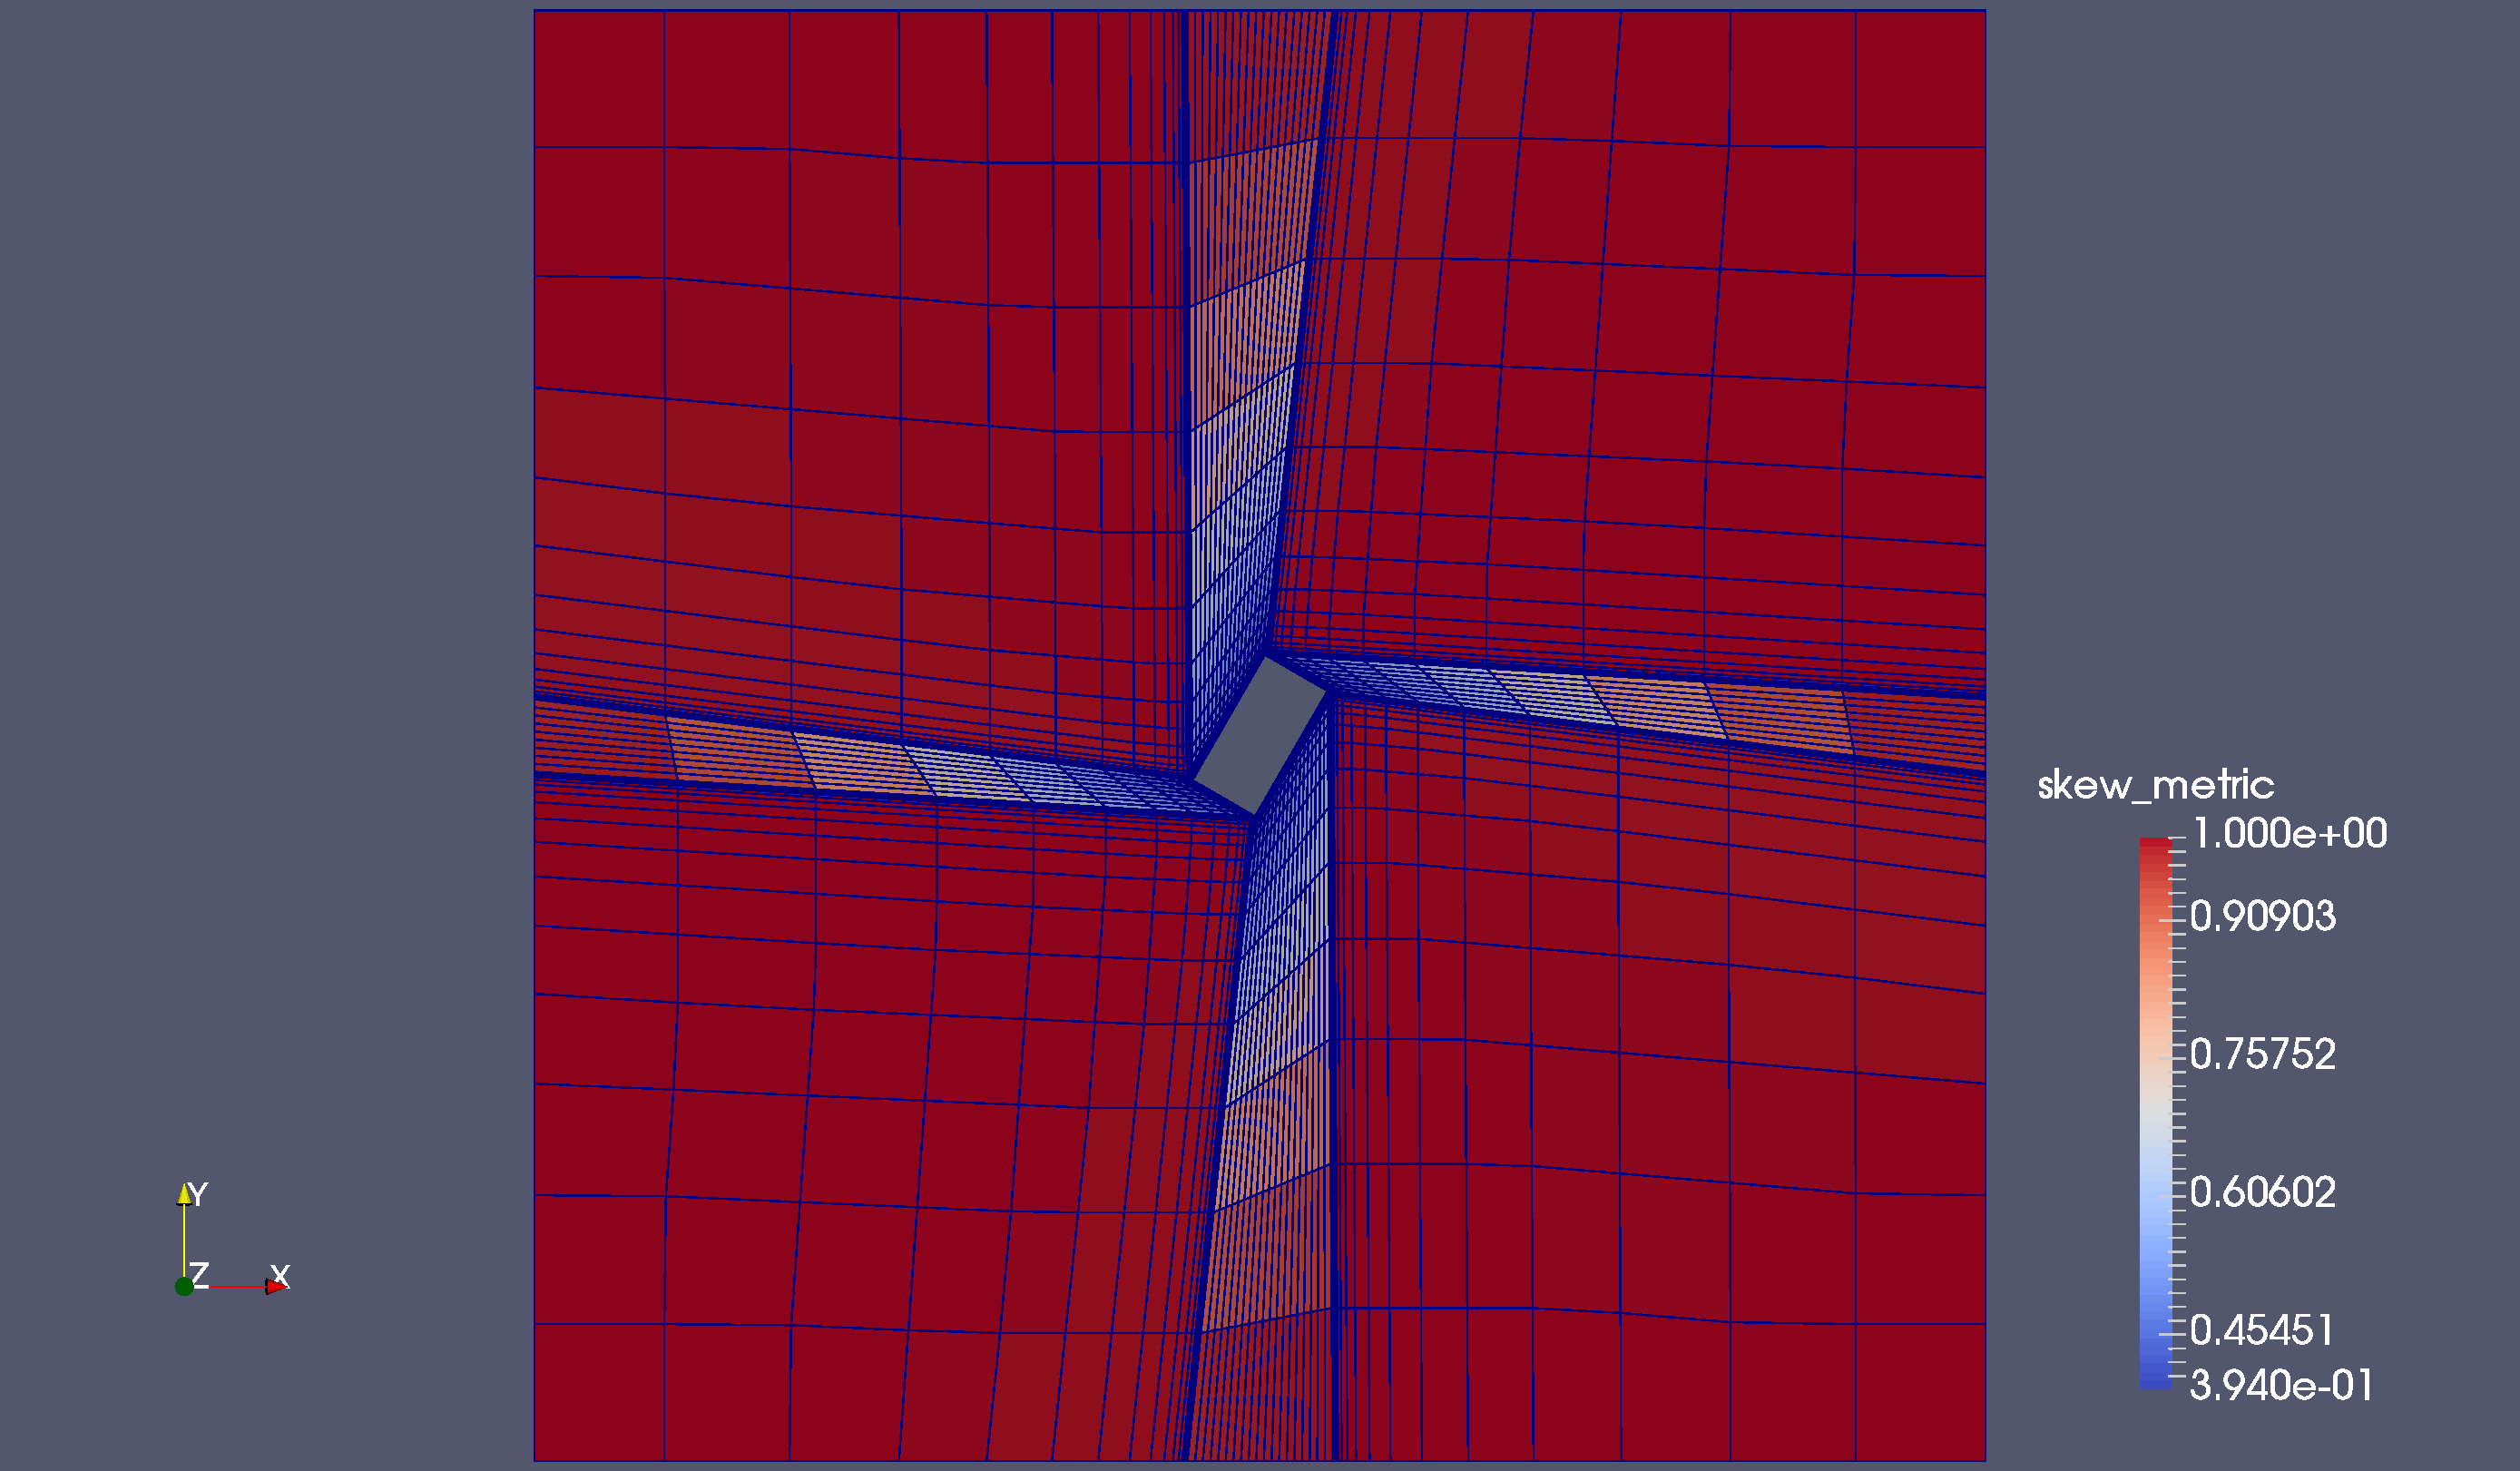
\includegraphics[scale=0.25]{qin-60-dgm-quality.pdf}
 	\caption{60 degrees rotation by DGM}
 	\label{fig:qin-60-dgm}
 \end{figure}
 
 \begin{figure}
 	\centering
 	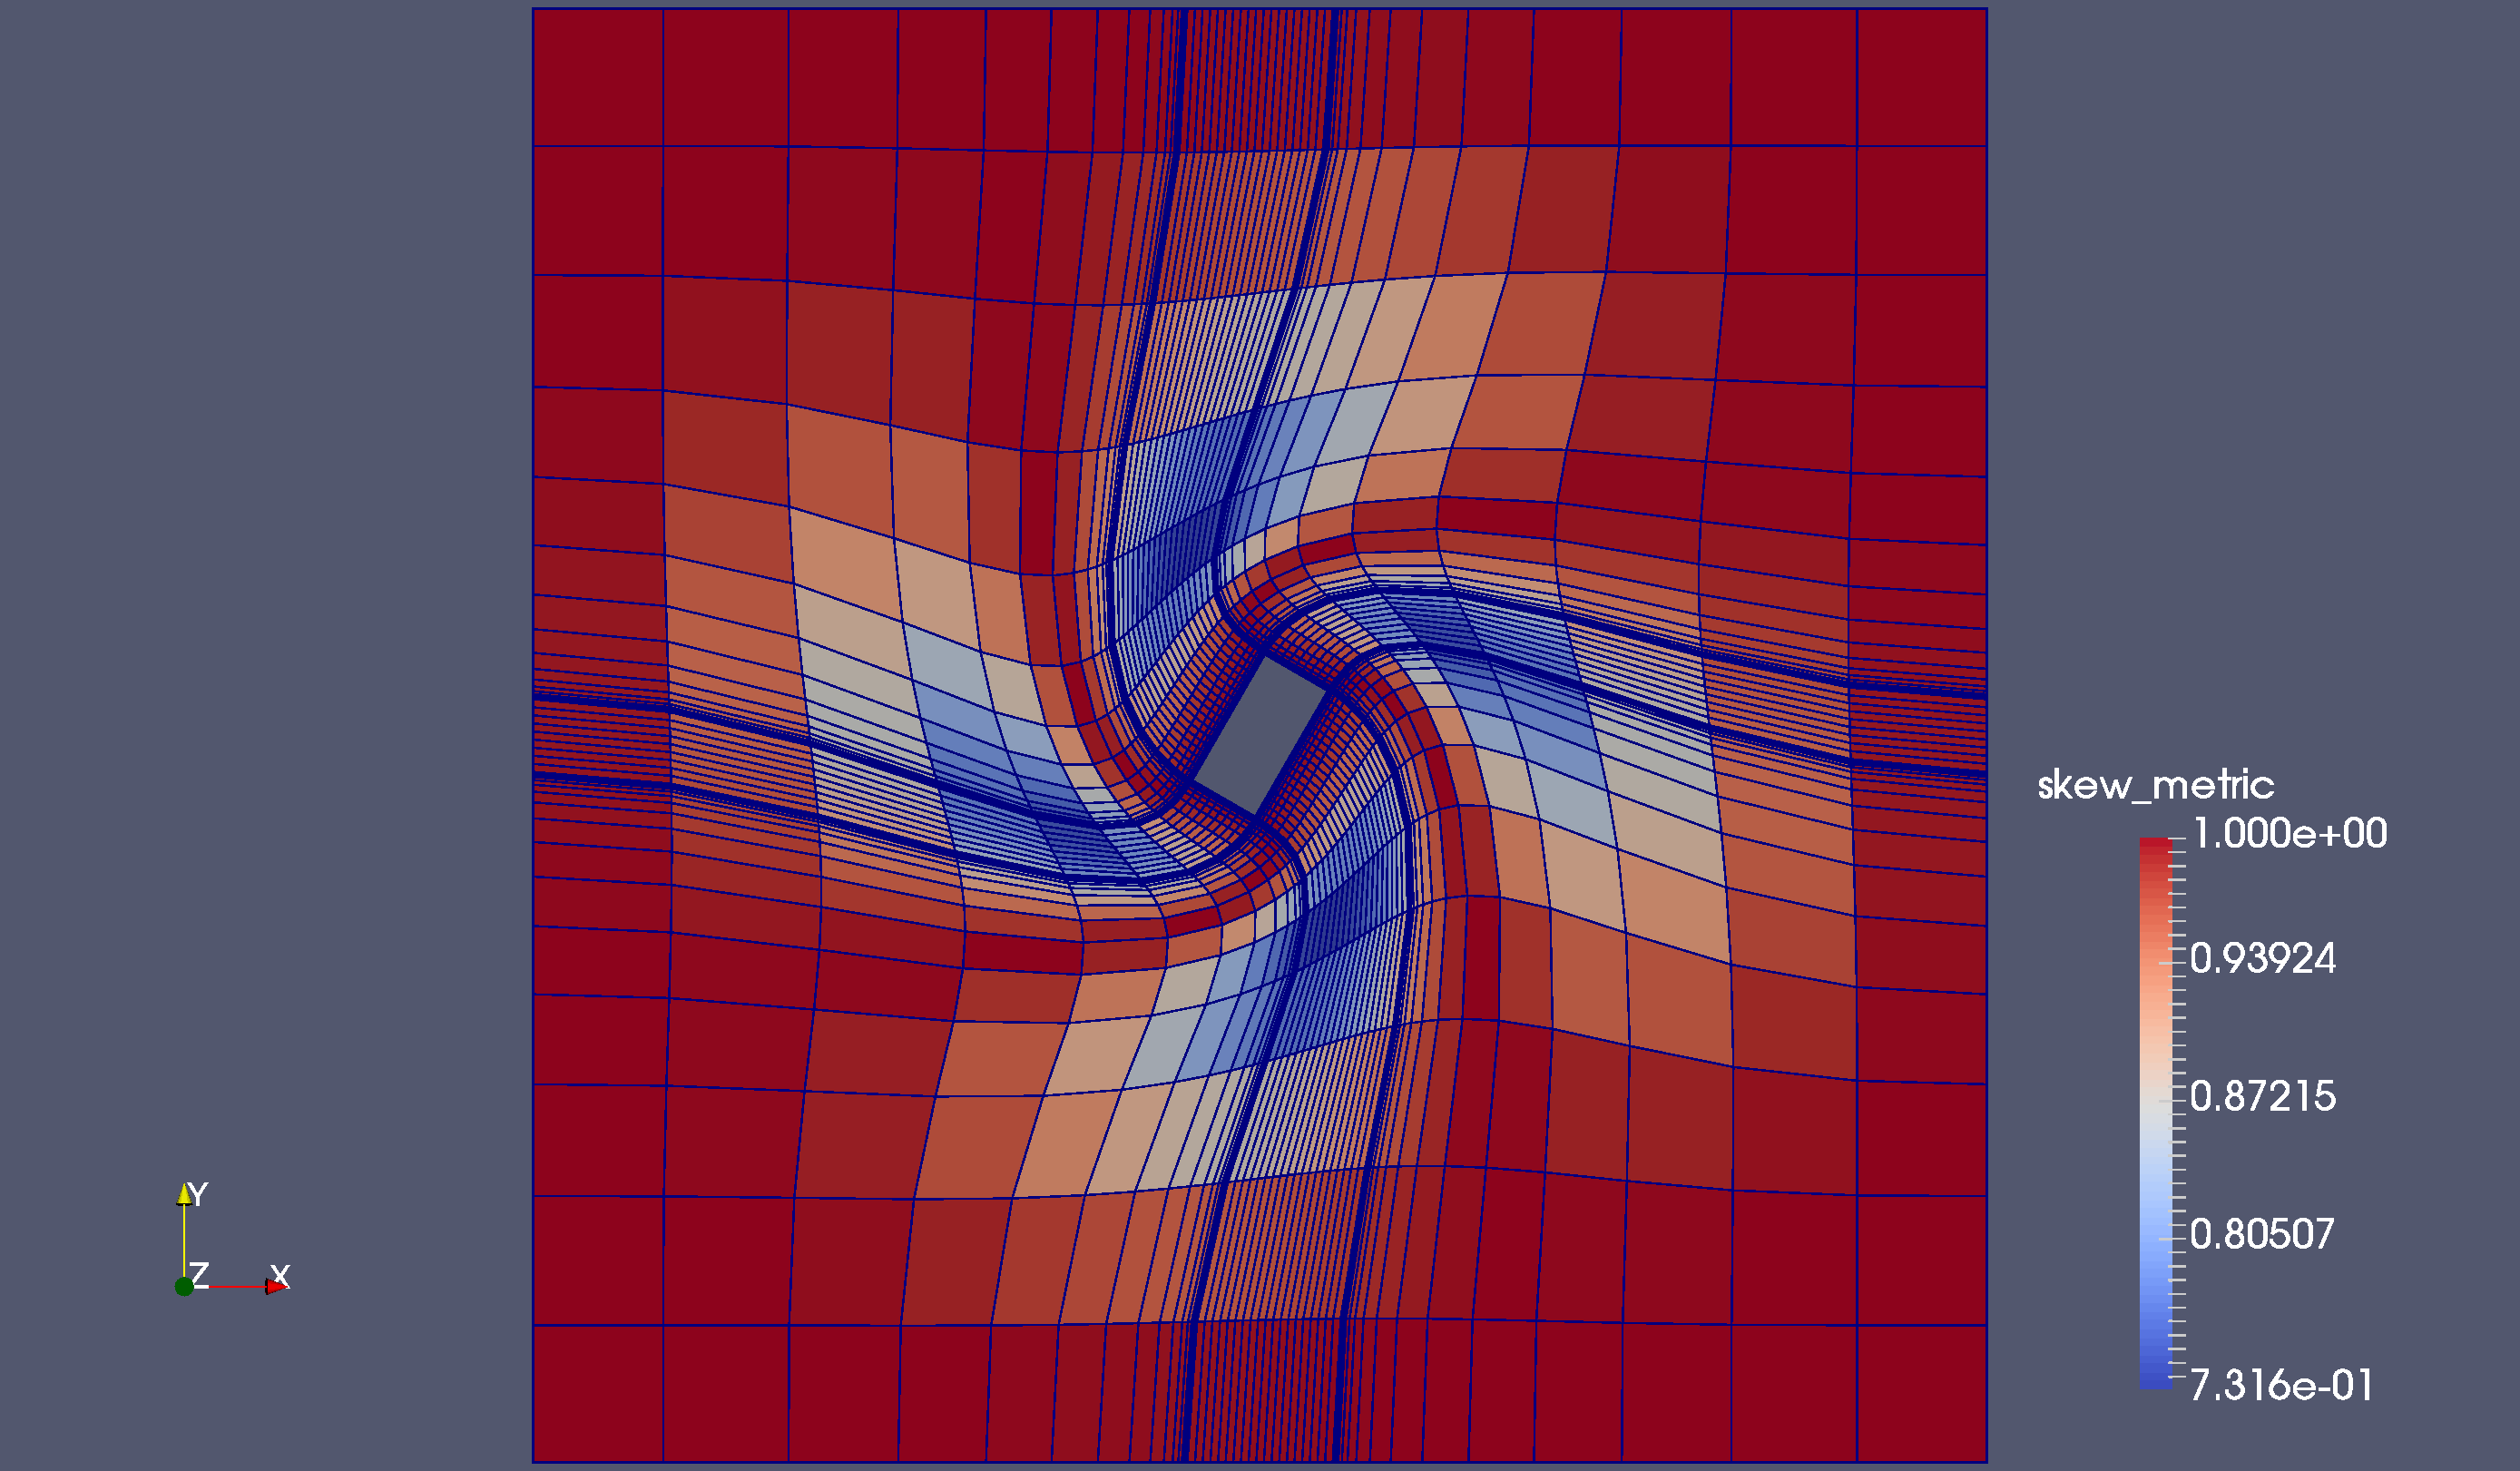
\includegraphics[scale=0.25]{qin-60-rbf-quality.pdf}
 	\caption{60 degrees rotation by RBF}
 	\label{fig:qin-60-rbf}
 \end{figure}
 
 \begin{figure}
 	\centering
 	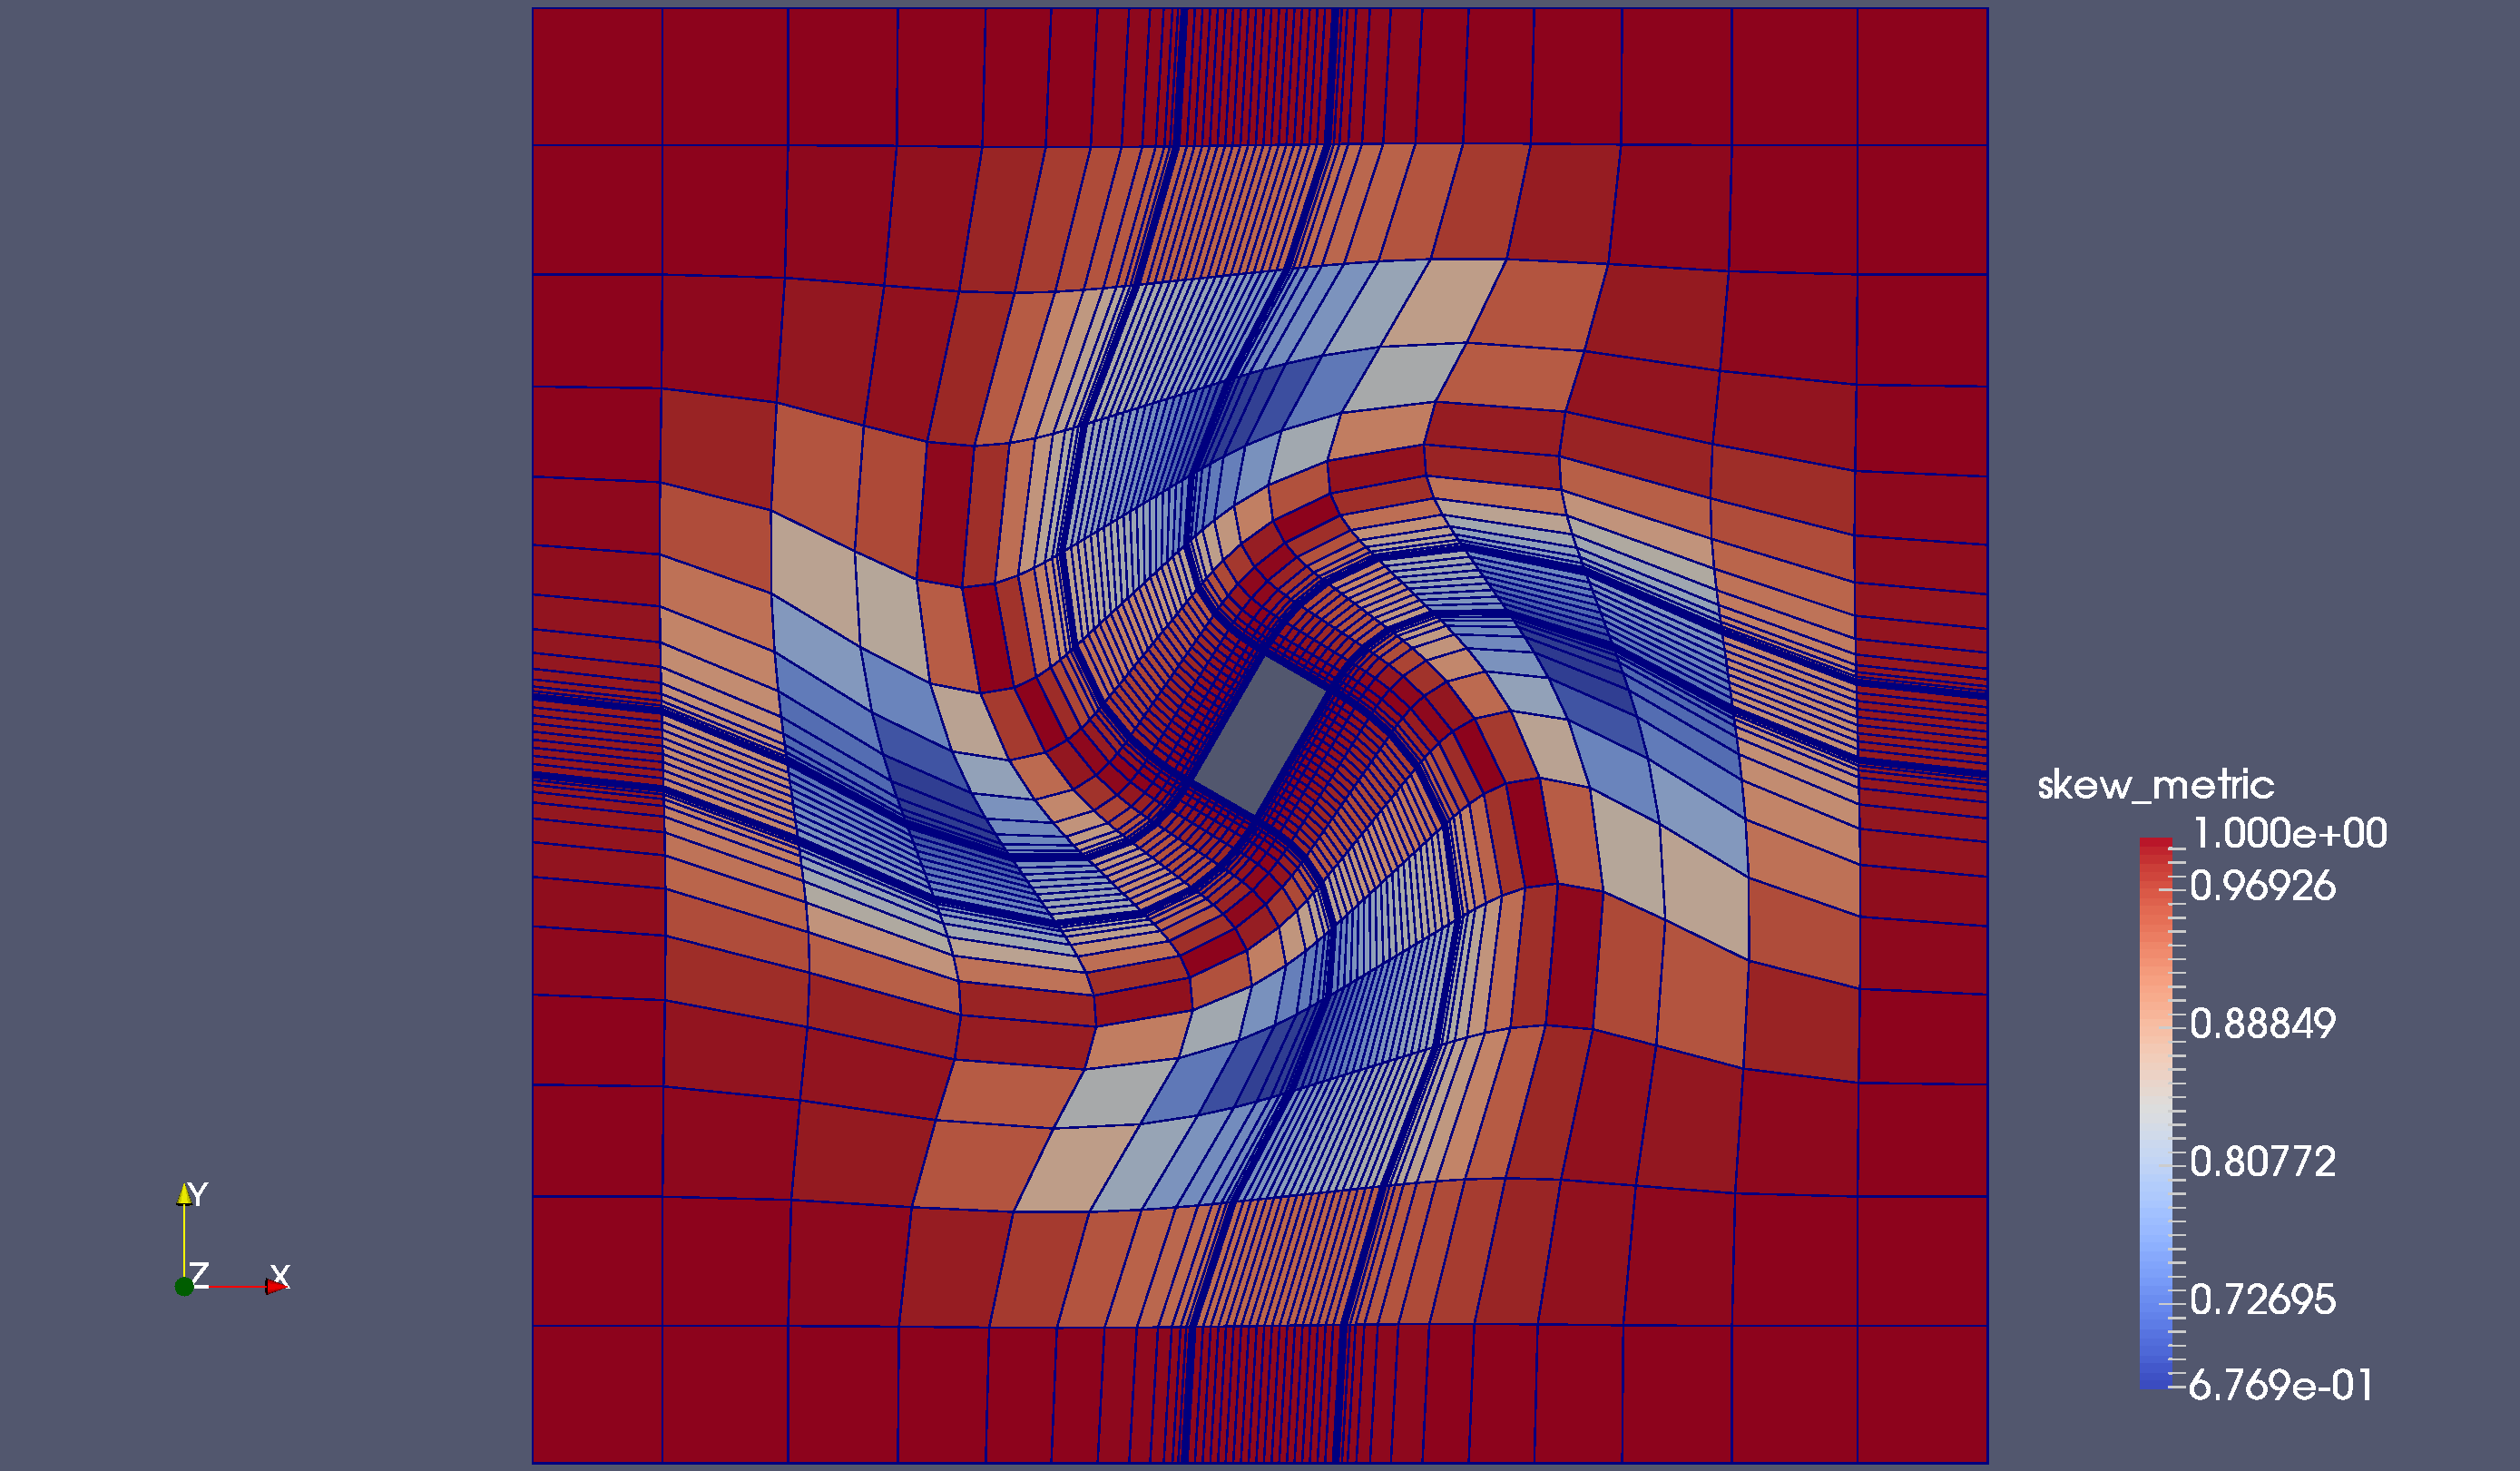
\includegraphics[scale=0.25]{qin-60-dgrbf2-quality.pdf}
 	\caption{60 degrees rotation by DGRBF2}
 	\label{fig:qin-60-dgrbf2}
 \end{figure}
 
 We note that the RBF and DGRBF2 methods can handle the rotation case quite well. The high-aspect-ratio elements near the inner boundaries are well-preserved, while the elements further in the interior, which are larger and can thus take more deformation, are distorted somewhat. Though RBF gives slightly better mesh quality than DGRBF2 for this amount of rotation, RBF takes 1.926 seconds of total CPU time (using conjugate gradient solver), while DGRBF2 takes only 0.08 seconds of total CPU time. Further, shown in figure \ref{fig:qin-dgrbf2-120} is a case of extreme rotation of 120 degrees, which DGRBF2 solves while maintaining mesh validity. None of the other methods are able to do this. RBF has been found to give valid meshes upto about 110 degrees of rotation. However, since DGRBF2 requires specification of rotation angles at boundary nodes, the method can be difficult to apply to general complex motions.
 
 \begin{figure}
 	\centering
 	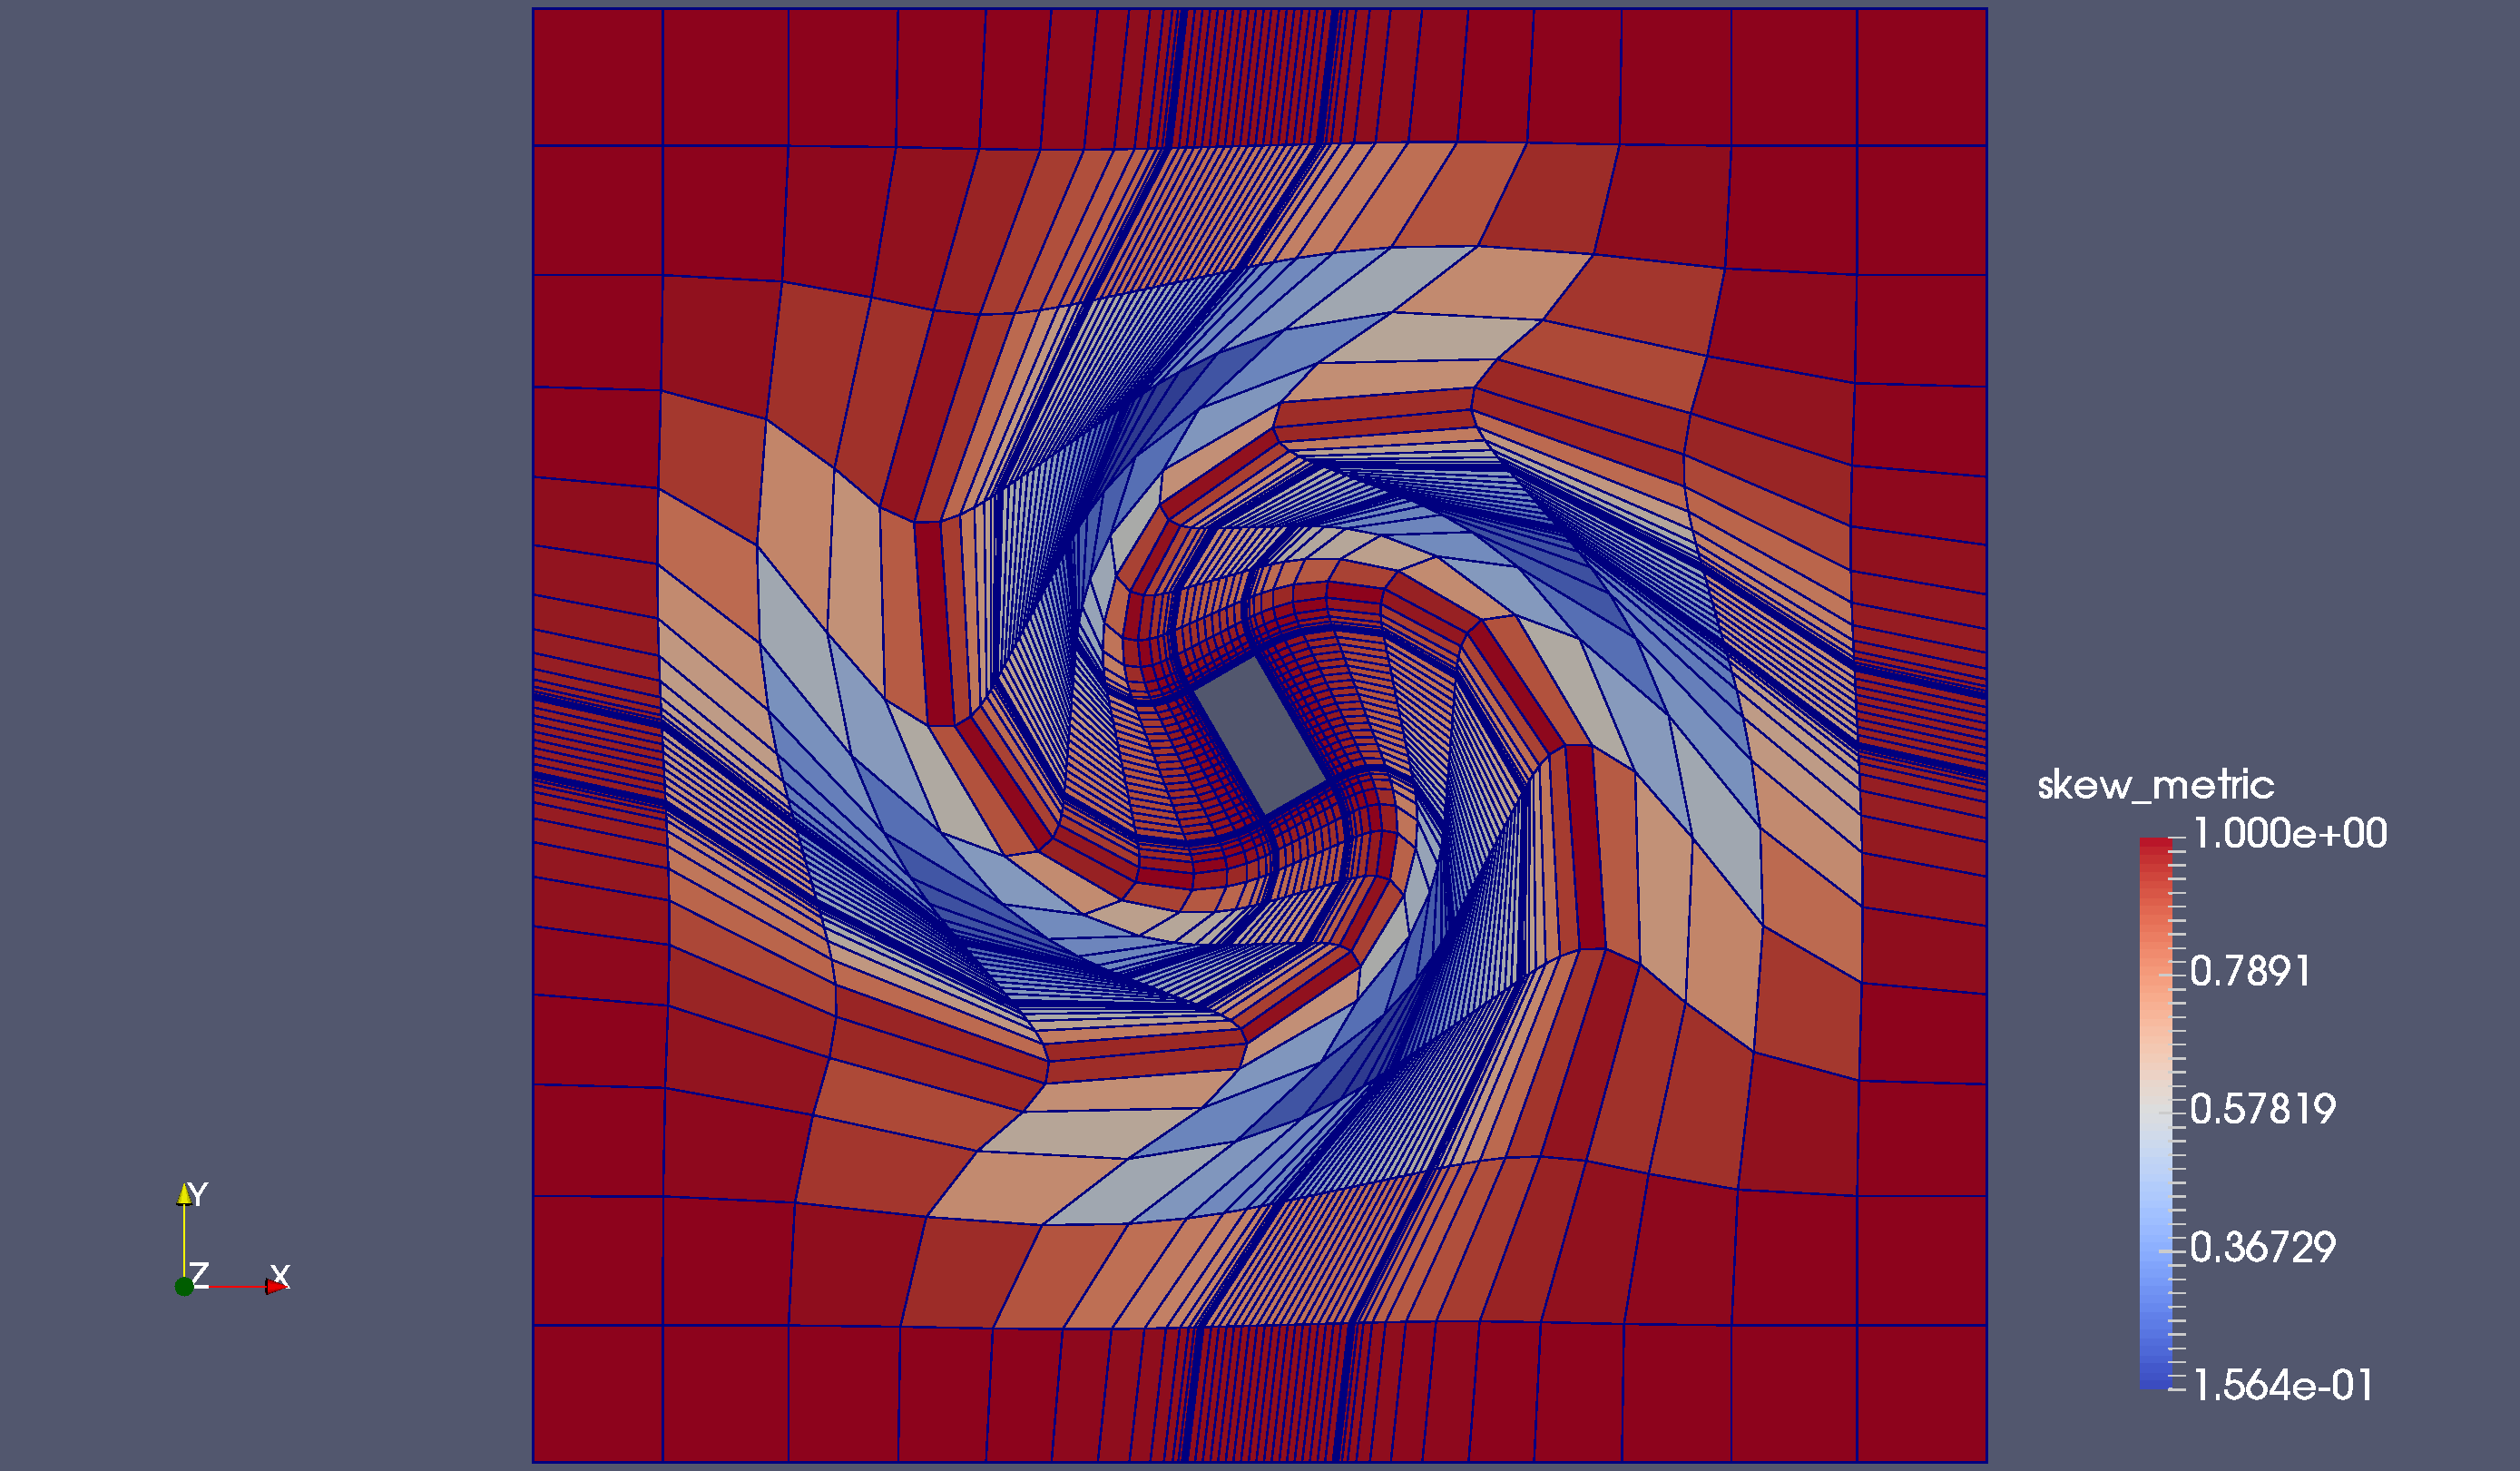
\includegraphics[scale=0.25]{qin-120-quality-withmesh.pdf}
 	\caption{Large rotational motion carried out by DGRBF2}
 	\label{fig:qin-dgrbf2-120}
 \end{figure}
 
 \FloatBarrier
 
 \section{Generation of curved meshes}
 
 Curved meshes for various standard viscous flow test cases have been generated with the method described in the previous section. These include flow past NACA0012 airfoil, flow through a bump channel and flow past a multi-element airfoil. Out of these, the mesh for the multi-element airfoil case is a truly unstructured mesh; the others are structured meshes which we first convert to unstructured format.
 
 The validity and quality of the generated mesh is established by computing the minimum scaled Jacobian determinant for each element. If the minimum value of the Jacobian determinant is zero or negative, the element is considered invalid. This is done as a post-processing step using the plugin `AnalyseCurvedMesh' available in Gmsh \cite{gmsh}. The quantity computed by this plugin is given as
 \begin{equation} 
 m_i = \frac{\inf_{\mathbf{x}\in\Omega_i}\det \mathbf{J}(\mathbf{x})}{\det \mathbf{J_l}_i},
 \end{equation}
 where $\mathbf{J}$ is the Jacobian matrix of the transformation of a reference element to the curved physical element, and $\mathbf{J_l}$ is the Jacobian of the transformation of the reference element to the linear (straight) physical element. $\Omega_i$ represents the \emph{i}th element.
 
 Here, we present results of 2D curved mesh generation in case of a multi-element airfoil. The mesh has triangular elements. It is meant for viscous flow computations and thus has highly stretched, thin elements near the wing boundaries. In this case, if the interior nodes are not moved properly, invalid elements result. In the figures, we compare curved meshes generated by isotropic linear elasticity and RBF interpolation. Both problems are solved using a Jacobi-preconditioned CG solver. Linear elasticity uses a Young's modulus $E$ of $1\times 10^6$ Pa and a Poisson's ratio of 0.4, though it is observed that the particular values do not influence the outcome much. A number of values over the range 1.0 to $1.0 \times 10^{10}$ were tried for $E$. RBF interpolation uses a support radius of 0.04 (for reference, the chord length of the wing is approximately 18.3).
 
 \begin{figure}
 	\centering
 	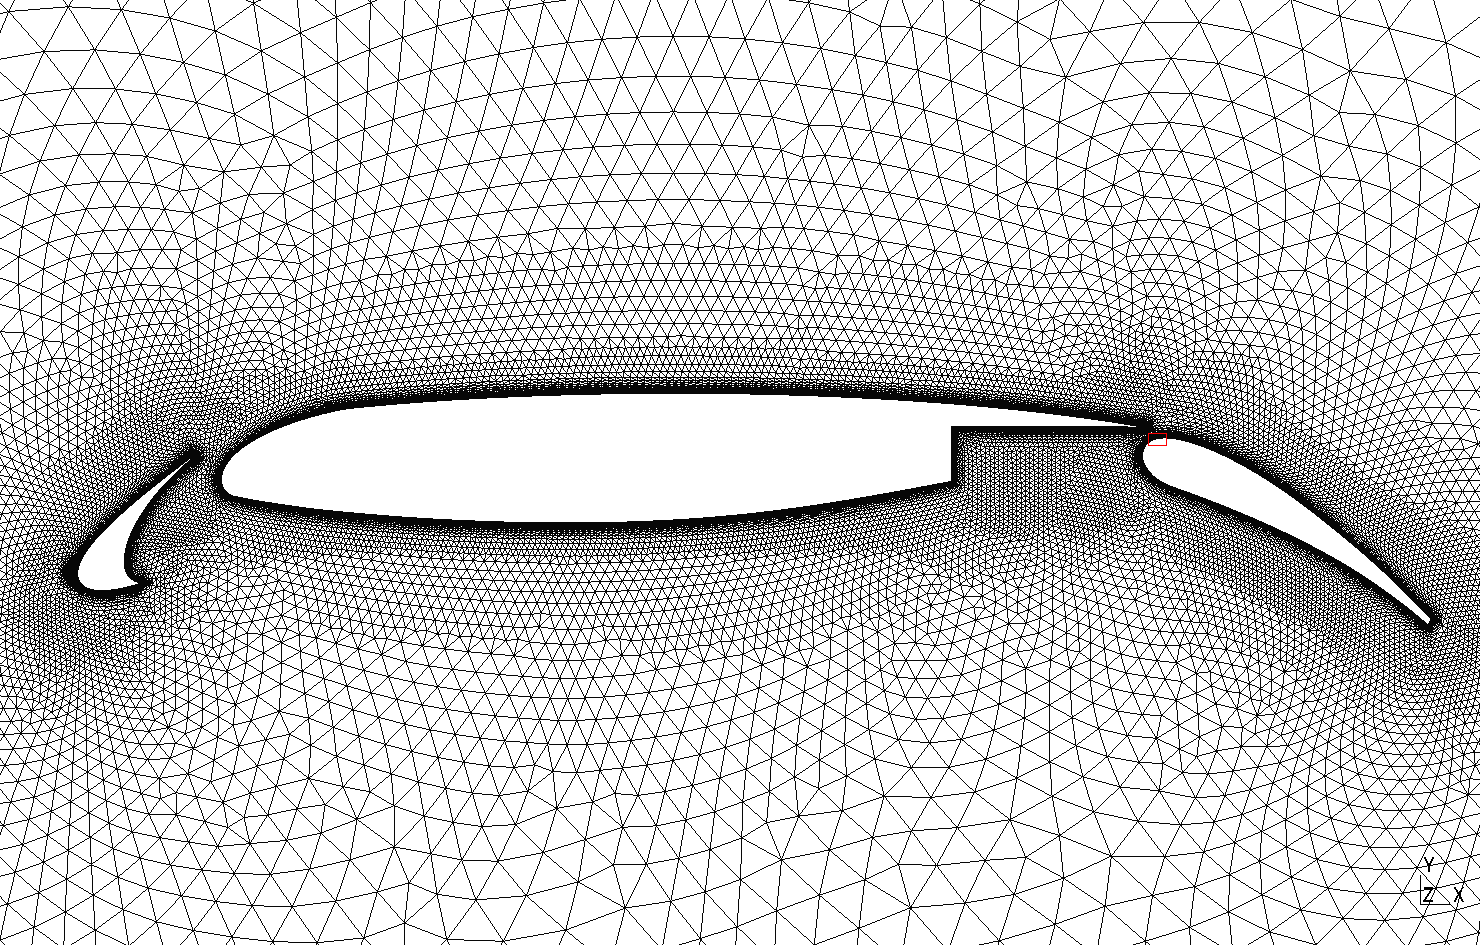
\includegraphics[width=300.0pt]{3compblack}
 	\caption{Mesh of multi-element airfoil. The little box shows approximately the region which is magnified in the figures that follow.}
 \end{figure}
 
 \begin{figure}
 	\centering
 	\subfloat{
 		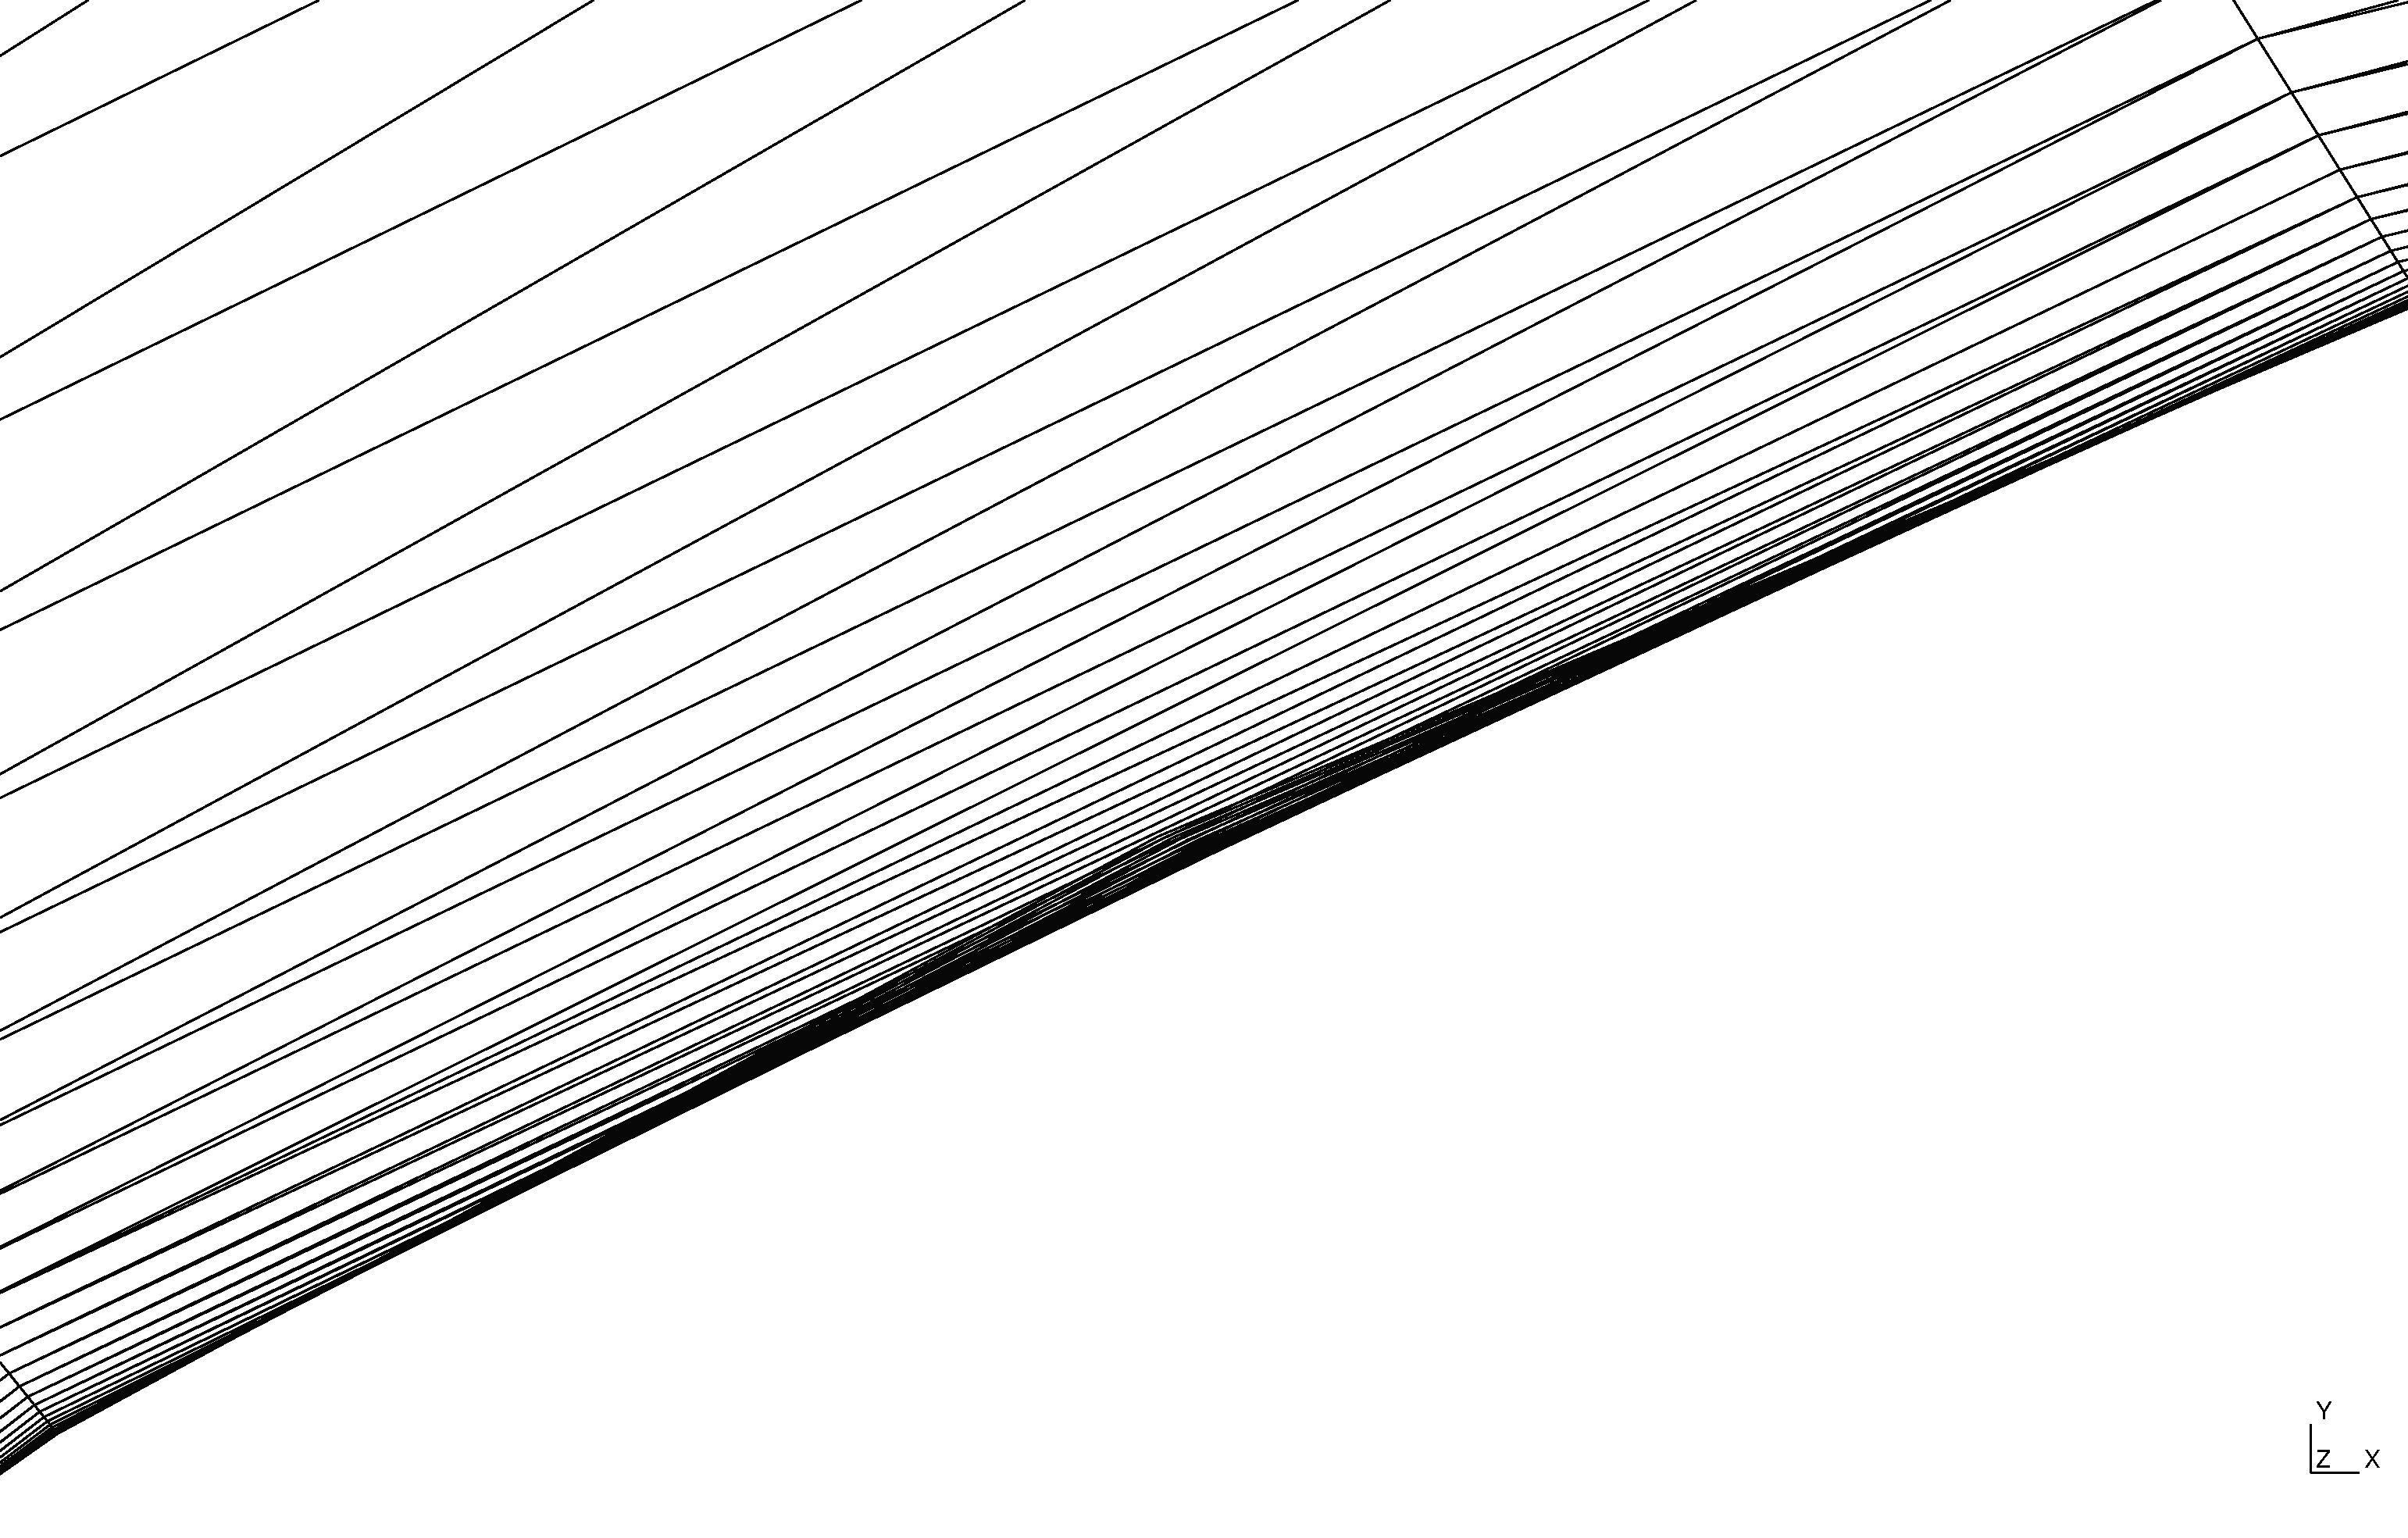
\includegraphics[width=200.0pt]{3comp-elast-zoomedblk.pdf}
 	}
 	\subfloat{
 		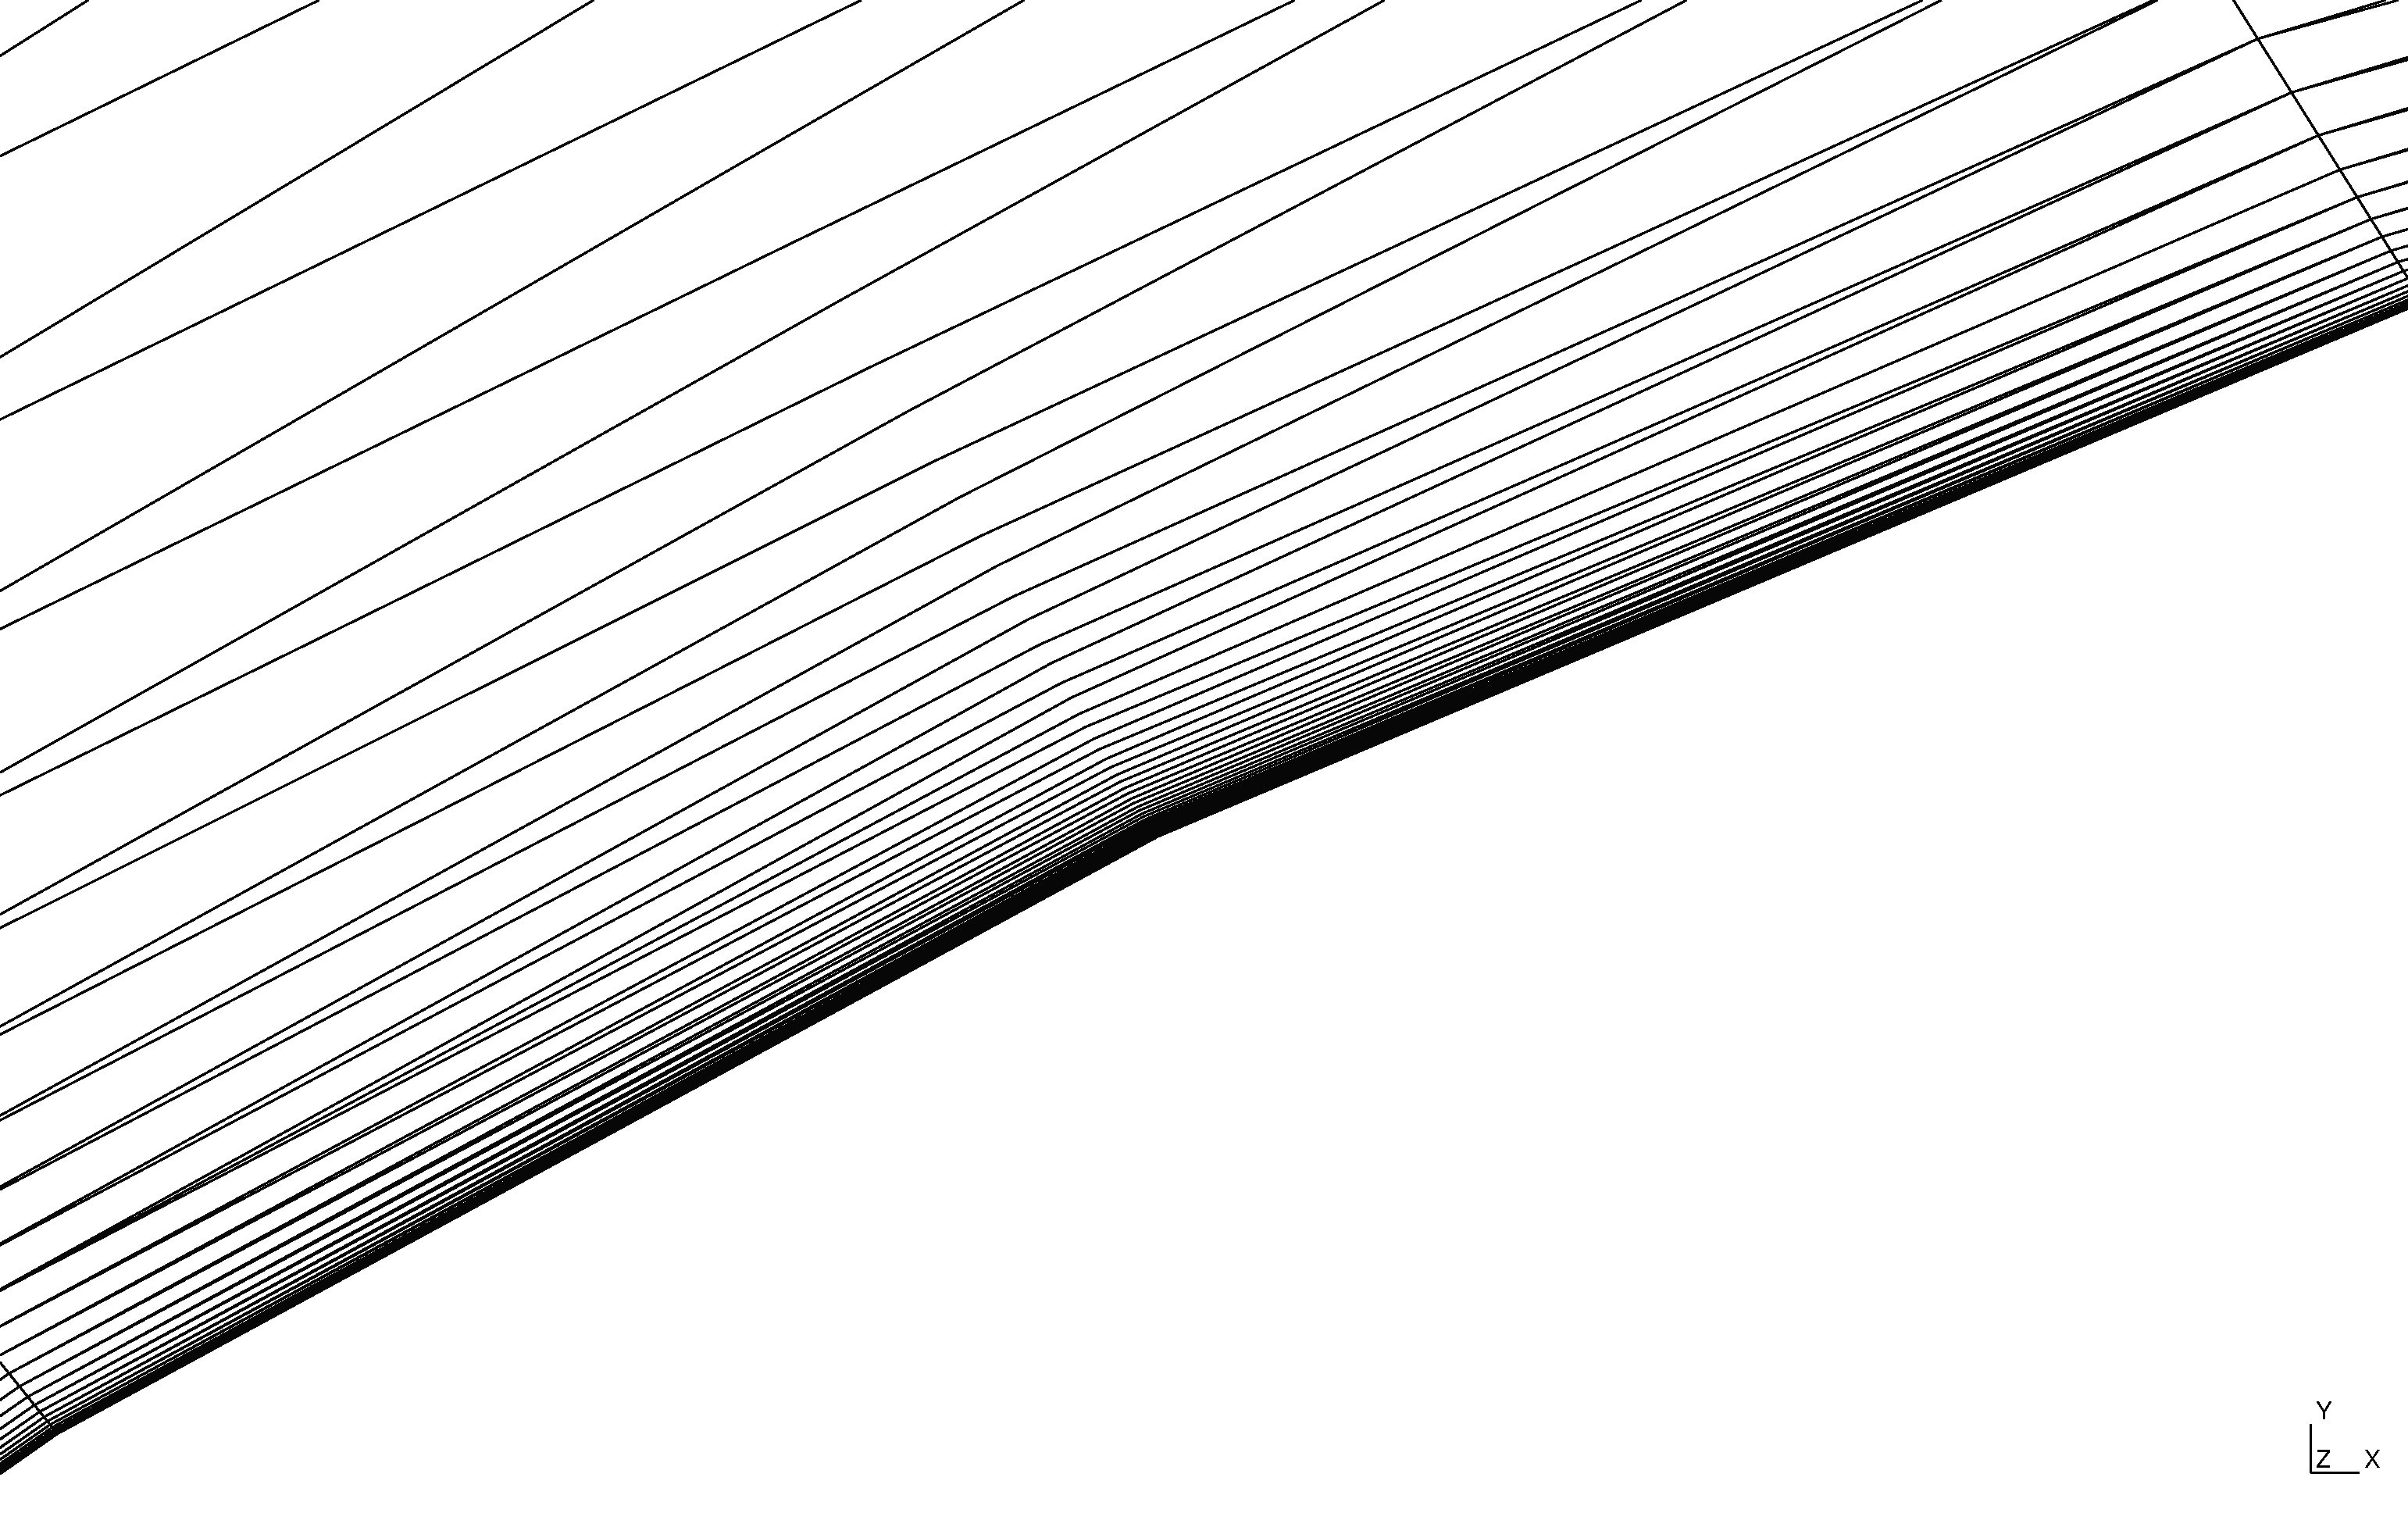
\includegraphics[width=200.0pt]{3comp-rbf-zoomedblk.pdf}
 	}
 	\caption{Portion of quadratic viscous mesh for multi-element airfoil, showing a boundary face in the flap, generated by linear elasticity (left) and RBF (right) methods.}
 	\label{fig:tangled1}
 \end{figure}
 
 \begin{figure}[!h]
 	\centering
 	\subfloat{
 		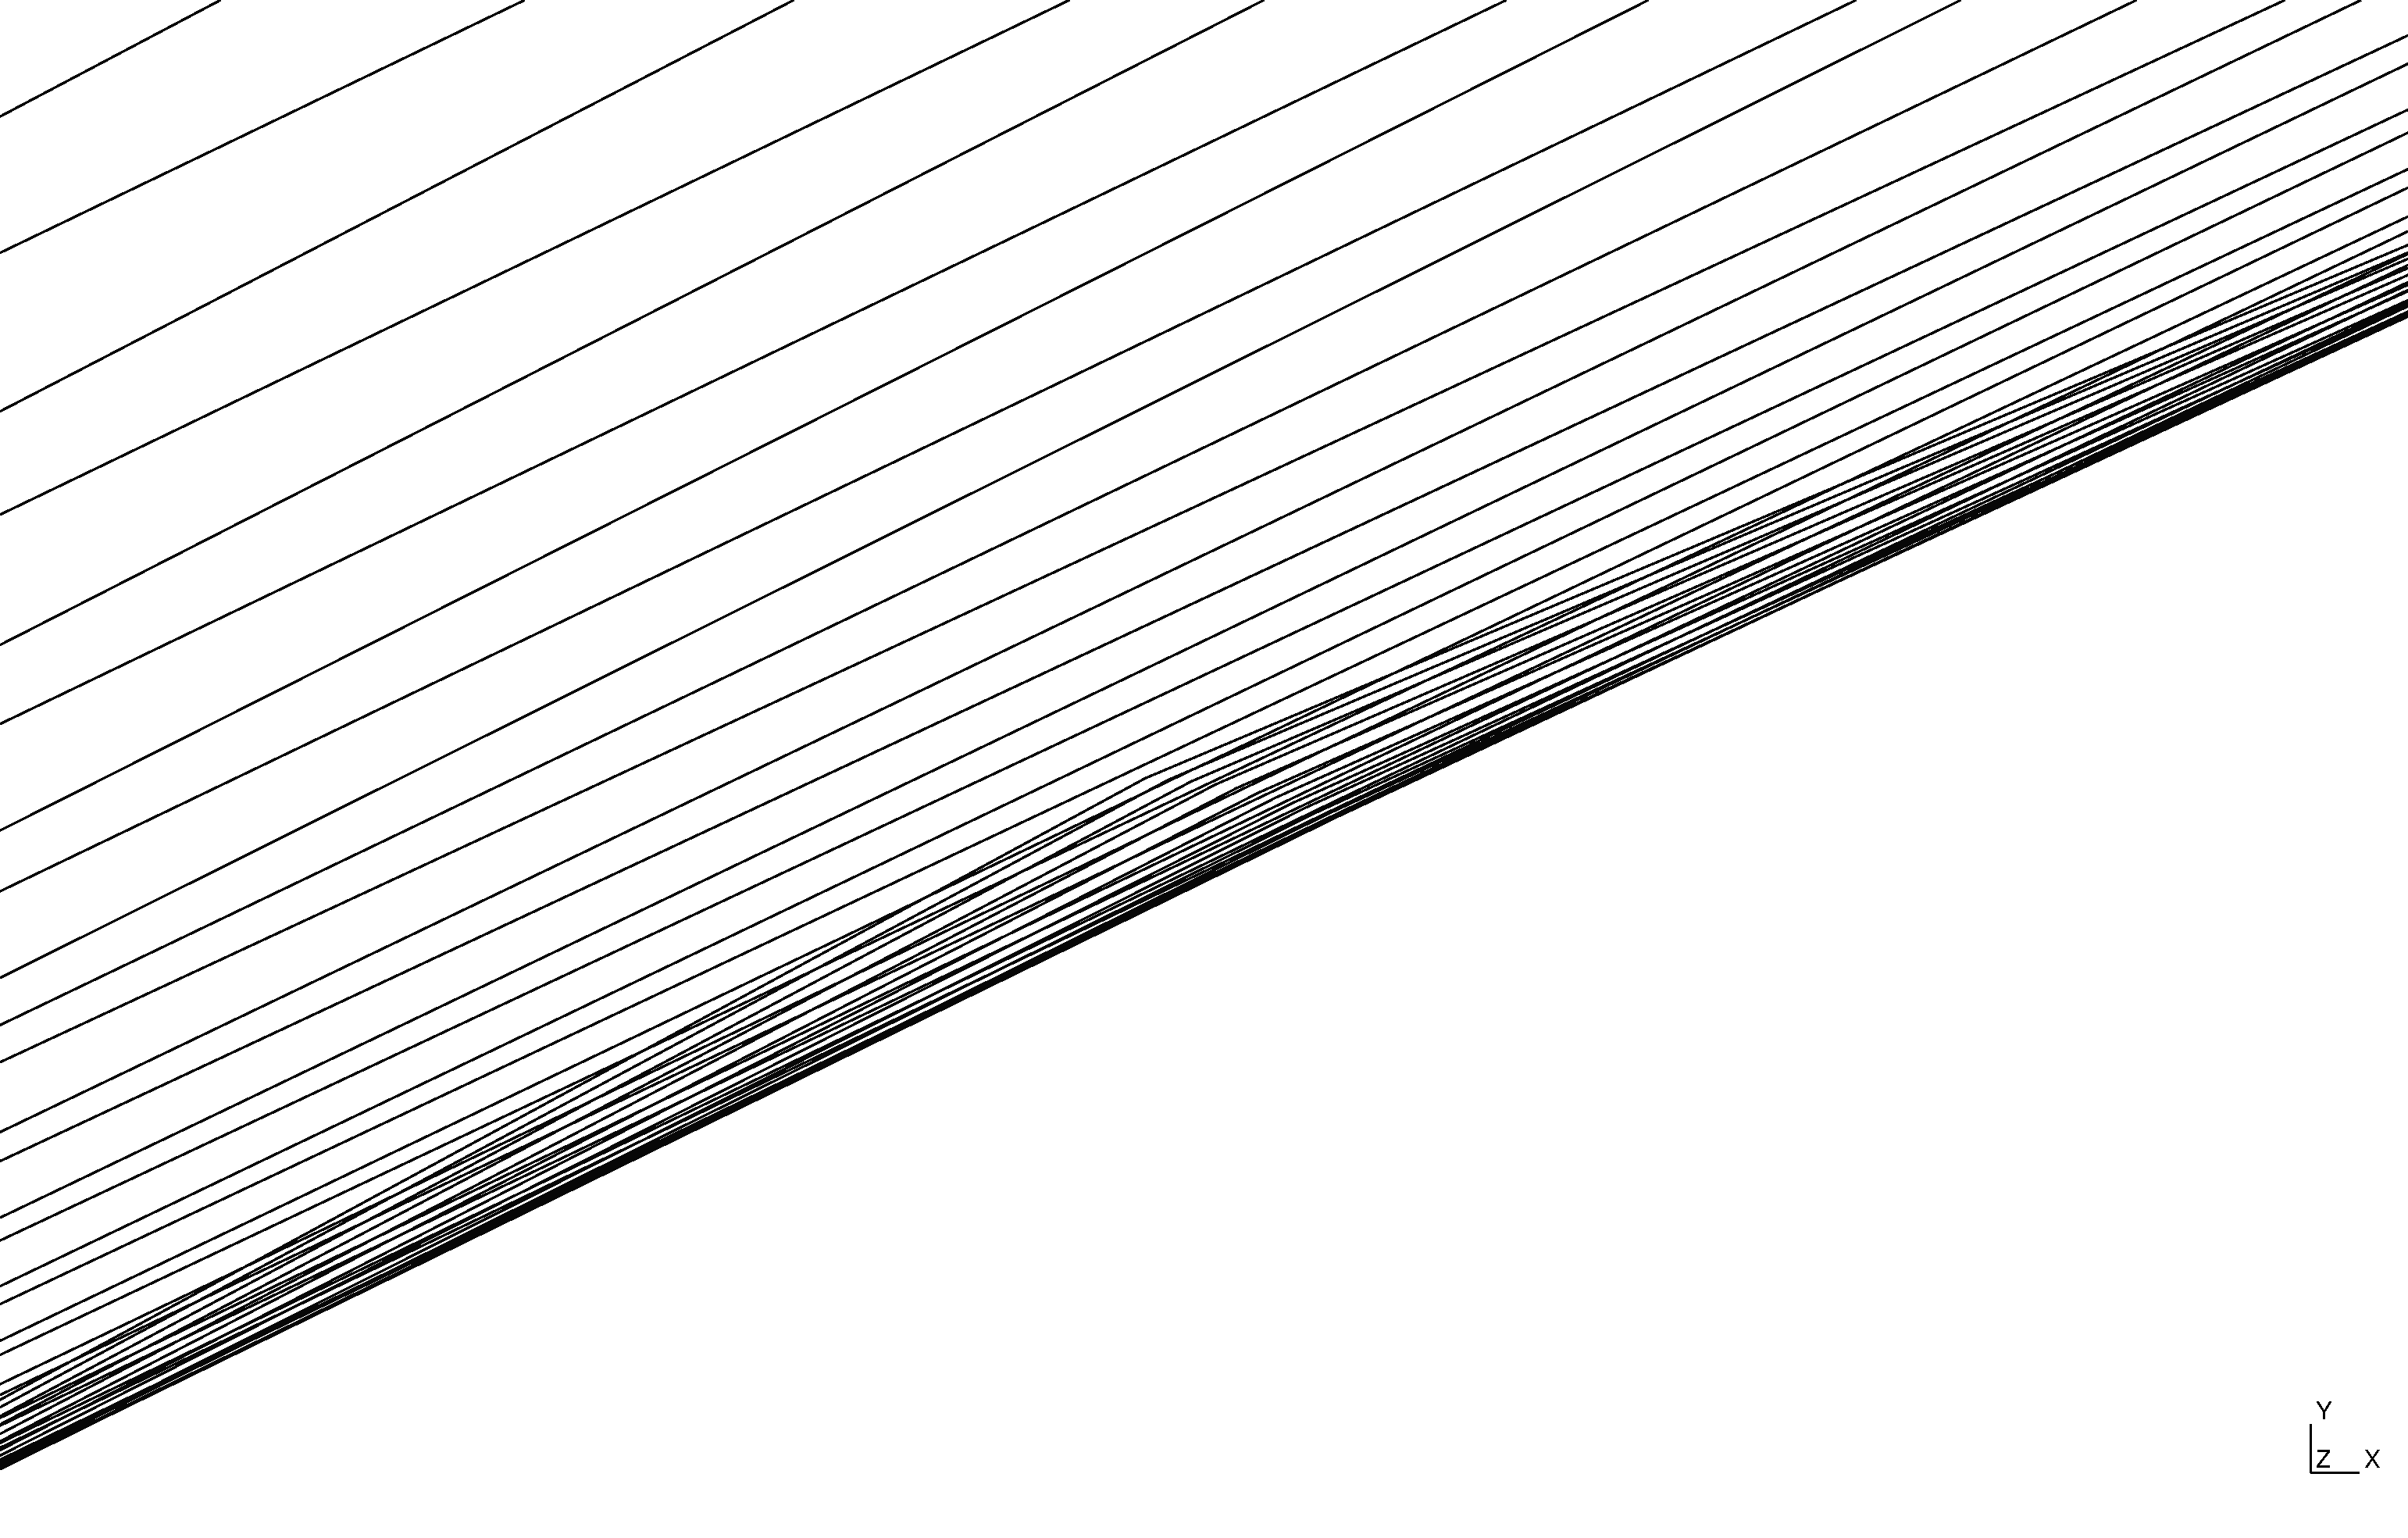
\includegraphics[width=200.0pt]{3comp-elast-vzoomedblk.pdf}
 	}
 	\subfloat{
 		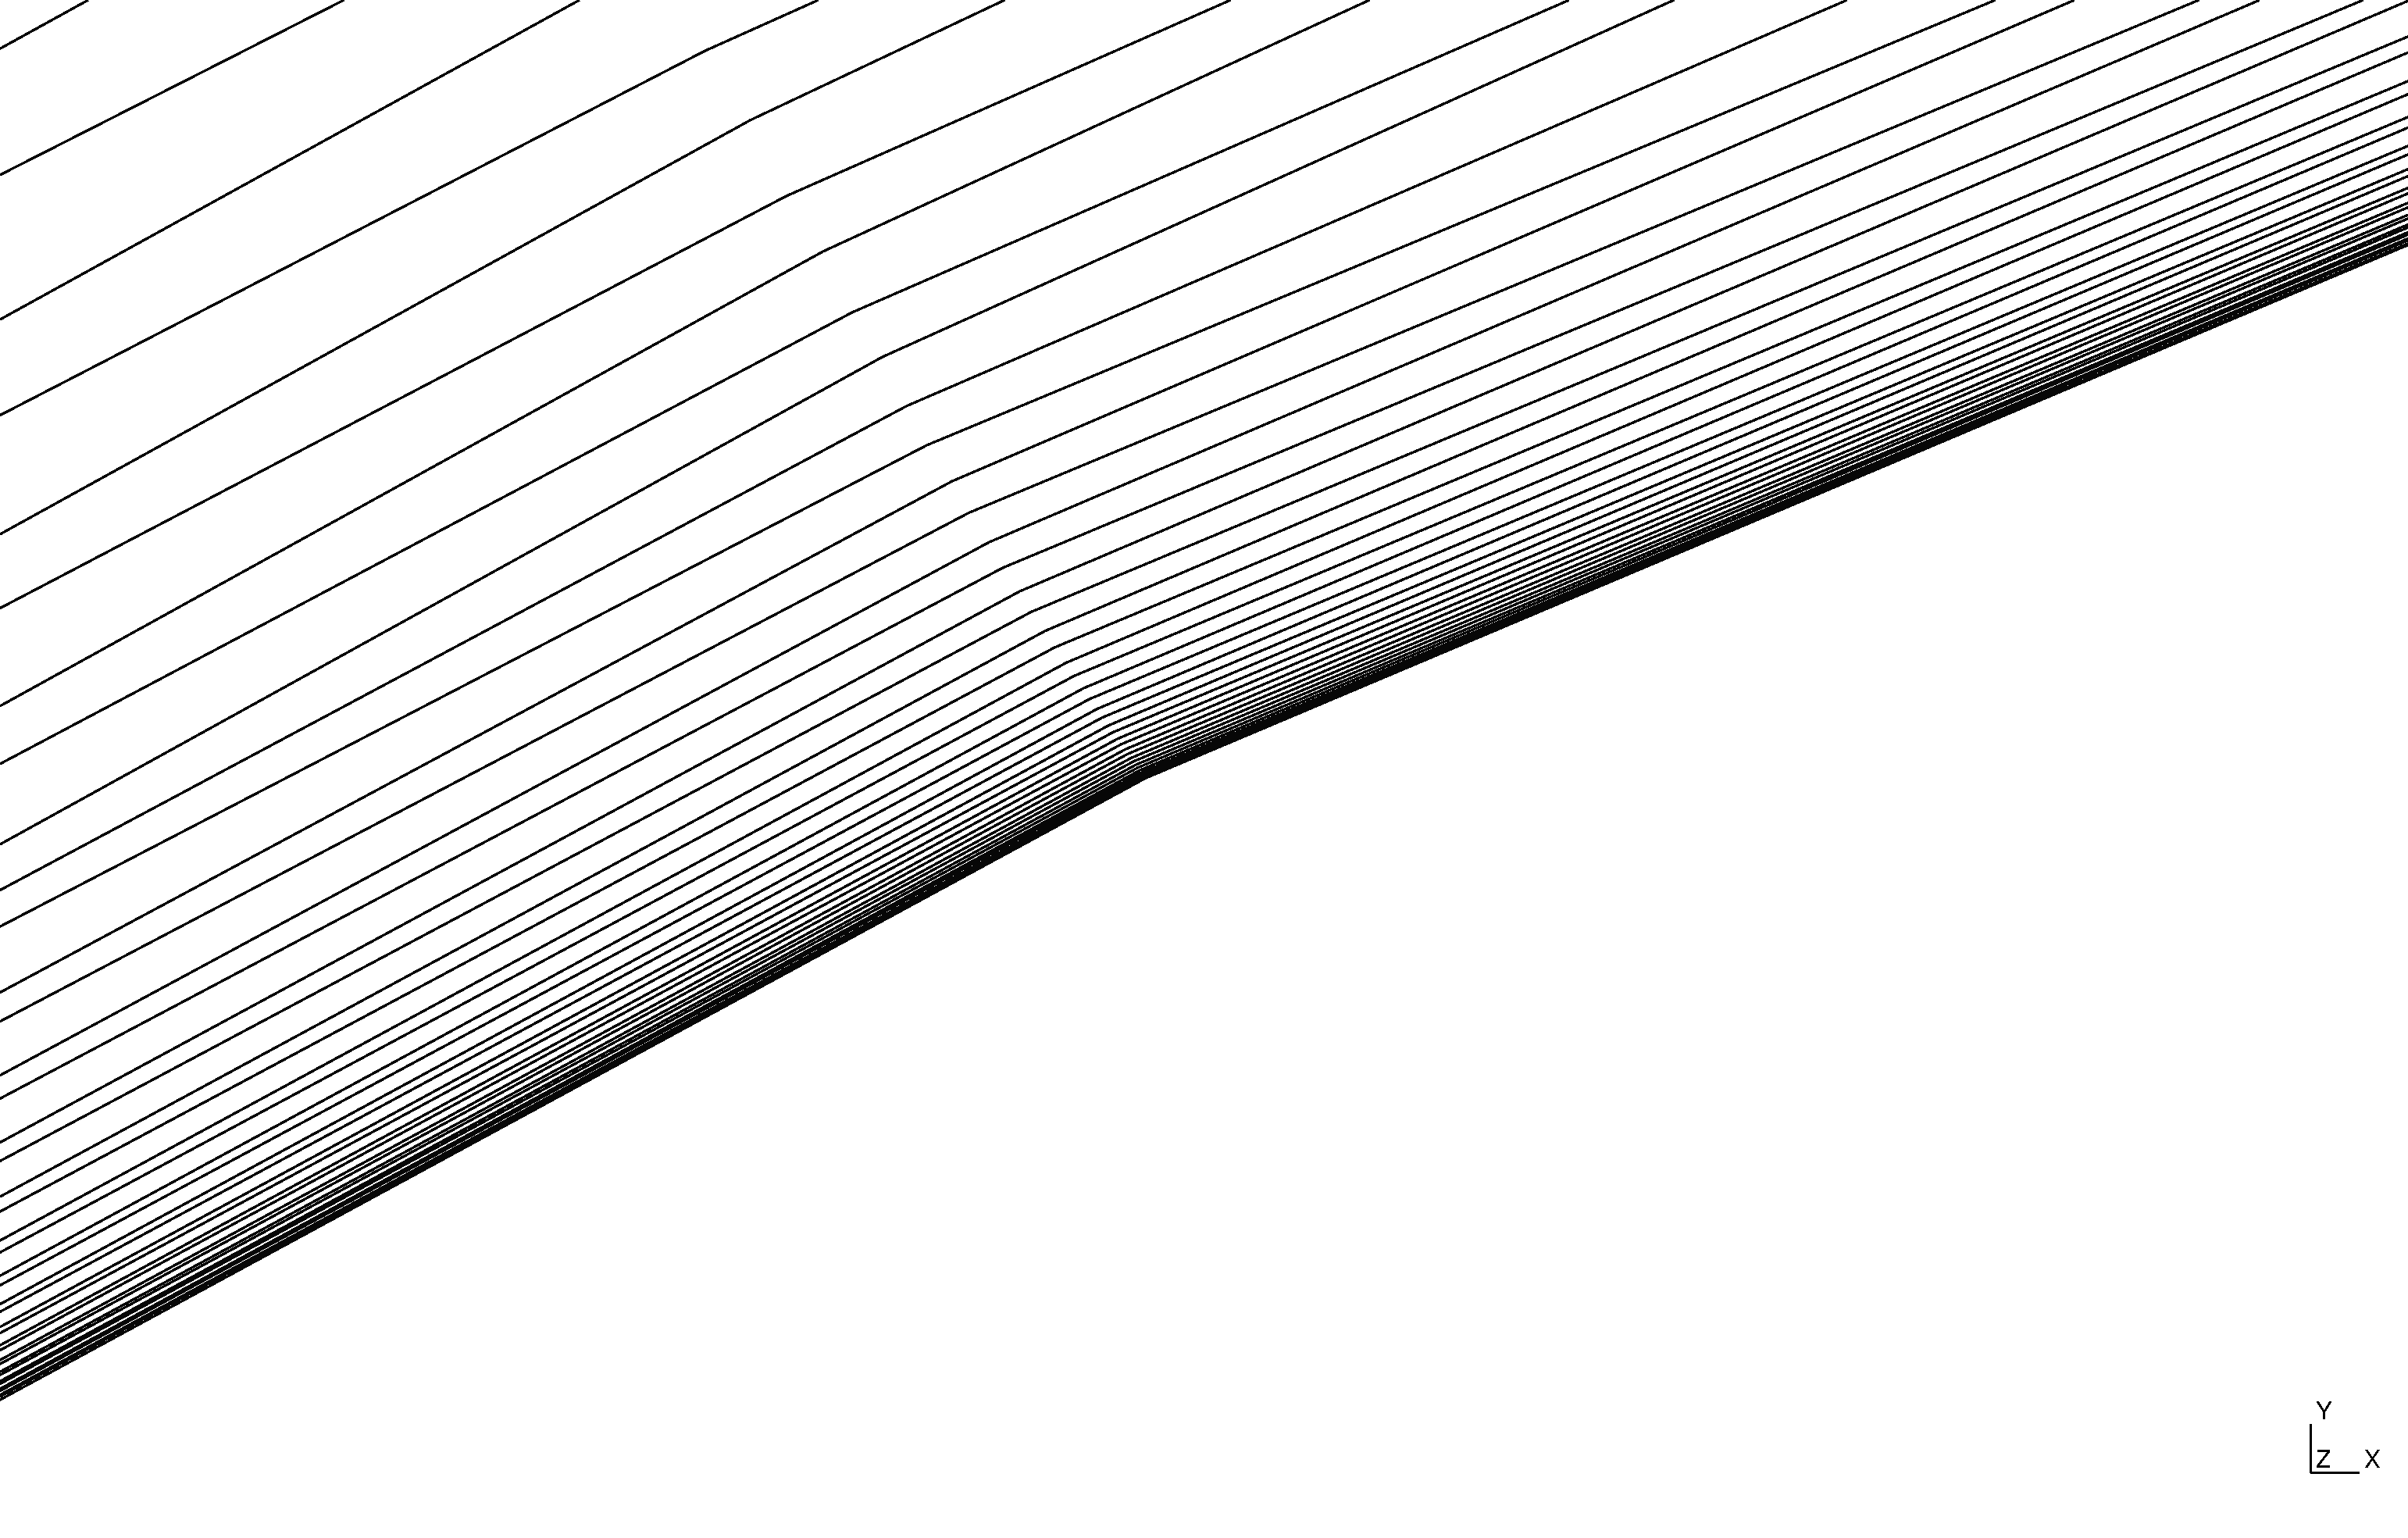
\includegraphics[width=200.0pt]{3comp-rbf-vzoomedblk.pdf}
 	}
 	\caption{Portion of quadratic viscous mesh for multi-element airfoil, showing a boundary face in the flap, generated by linear elasticity (left) and RBF (right) methods. Both are zoomed to for a clearer view.}
 	\label{fig:tangled2}
 \end{figure}
 
 In figures \ref{fig:tangled1} and \ref{fig:tangled2}, the first mesh is tangled; even though the nodes are being moved, they are not being moved far enough. It is clear that simple linear elasticity is not enough for curved mesh generation - we get negative Jacobians in several near-boundary elements for many curved boundary faces. However, the RBF method is satisfactory, with a scaled minimum Jacobian range of 0.64 to 1.0 throughout the mesh (figure \ref{fig:rbf-jacobians}). As explained earlier, we see that the elements very close to the boundary deform very little - they have scaled Jacobian nearly 1.0. As we go further from the boundary, the Jacobian drops to a minimum and then rises again to 1.0 at a distance that approximately equals the support radius.
 
 \begin{figure}
 	\centering
 	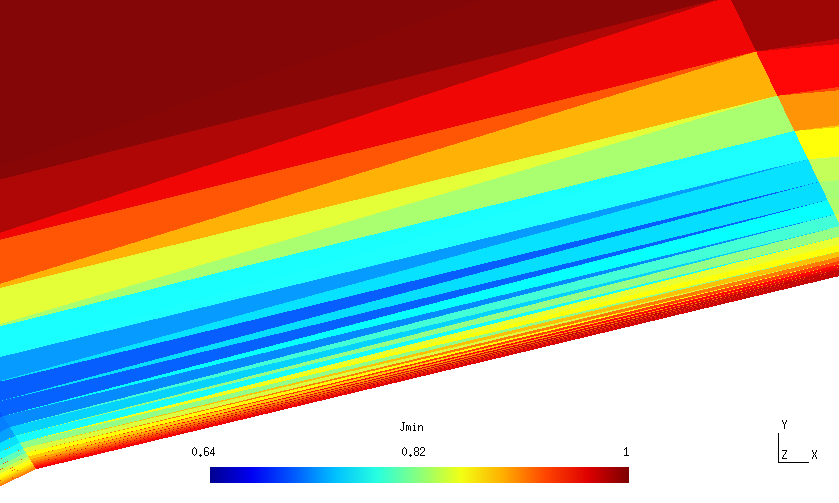
\includegraphics[width=400pt,scale=0.5]{3comp-rbf-zoomed-jacobians2.png}
 	\caption{Minimum scaled Jacobian over each element for mesh generated by RBF interpolation. (The mesh is actually curved, though the graphics of Gmsh ignore that.)}
 	\label{fig:rbf-jacobians}
 \end{figure}